\documentclass{article}

\usepackage[round]{natbib}
\usepackage[english]{babel}
\usepackage[letterpaper,top=2cm,bottom=2cm,left=3cm,right=3cm,marginparwidth=1.75cm]{geometry}

\usepackage{booktabs}
\usepackage{tabularx}
\usepackage{authblk}
\usepackage{amsmath}
\usepackage{amsfonts}
\usepackage{graphicx}
\usepackage{makecell}
\usepackage{url}
% For rotating figures, tables, etc.
%  including their captions - only for supplementary figures
\usepackage{rotating}

% JK: turning this off for the moment as I keep clicking through on links
% to the bibliography while reading the text and it's intensely annoying.
% Can reinstate when we're ready to preprint
% \usepackage[hidelinks]{hyperref}


\title{Towards Pandemic-Scale Ancestral Recombination Graphs of SARS-CoV-2}
\author[1]{Shing H. Zhan}
\author[2,5]{Katherine Eaton}
\author[3,5]{Anastasia Ignatieva}
\author[1,5]{Benjamin Jeffery}
\author[1,5]{Duncan S. Palmer}
\author[1,5]{Yan Wong}
\author[2]{Carmen L. Murall}
\author[4]{Sarah P. Otto}
\author[1,6]{Jerome Kelleher}
\affil[1]{Big Data Institute, Li Ka Shing Centre for Health Information and Discovery, University of Oxford, Oxford, United Kingdom}
\affil[2]{National Microbiology Laboratory, Public Health Agency of Canada, Canada}
\affil[3]{Department of Statistics, University of Oxford, Oxford, United Kingdom}
\affil[4]{Department of Zoology and Biodiversity Research Centre, University of British Columbia, Vancouver, British Columbia, Canada}
\affil[5]{Preliminary alphabetic ordering}
\affil[6]{Correspondence. E-mail: jerome.kelleher@bdi.ox.ac.uk}

\begin{document}
\maketitle

\begin{abstract}
Recombination is an important and ongoing feature of SARS-CoV-2 evolution,
and presents major challenges to [things important to public health].
Detection of new recombinant strains is challenging, with methods
[being a bit rubbish].
In addition, many basic approaches fundamental to the study of viral
evolution assume that recombination is negligible, in that a single
phylogenetic tree can represent the genetic ancestry of the
circulating strains. Here we present an initial version of
\texttt{sc2ts}, a method to automatically detect recombinants
in real-time and to fully integrate them into a cohesive joint
model of mutation, recombination and genetic inheritance known
as an Ancestral Recombination Graph (ARG). We infer two ARGs under
different sampling strategies, and study their properties.
One contains 1.27 million sequences
sampled up to June 30, 2021, and the second is more sparsely sampled,
consisting of 784K sequences sampled up to June 30, 2022.
We find that both ARGs are
% better words?
highly consistent with
known features of SARS-CoV-2 evolution, recovering the basic
backbone phylogeny, mutational spectra, and recapitulating
details on the majority of known recombinant lineages.
Using the well-established and feature-rich \texttt{tskit} library,
the ARGs can also be stored concisely and processed efficiently
using standard Python tools. For example, the ARG for 1.27 million
sequences---encoding the inferred reticulate ancestry,
genetic variation, and extensive metadata---requires
58MB of storage,
and loads in less than a second.
%JK Not sure if we'd actually say it like this, but this is the
% basic gist I'd like to get accross[
The ability to fully integrate the effects of recombination into
downstream analyses, to quickly and automatically detect new recombinants,
and to provide an efficient and convenient platform for computation
makes \texttt{sc2ts} a promising approach, worthy of
further investment and development.
\end{abstract}

\section{Introduction}
% Recombination is an important force in SARS-CoV-2, recombinants
% have arisen and they have spread to high frequencies
Recombination via template switching is a common feature
of the evolution of coronaviruses~\citep{Graham2010-xe,De_Klerk2022-tt},
including SARS-CoV-2
\citep{VanInsberghe2021-eu,Jackson2021-ik,Ignatieva2021-rg}. By bringing
together mutations carried by different lineages, recombination plays an
important role in generating genetic diversity, with recombinant lineages
associated with adaptation to new host species and with the production of more
immune evasive variants~\citep{Graham2010-xe,De_Klerk2022-tt}.
% Early in the SARS-CoV-2 pandemic there was insufficient
% genetic variation for meaningful recombination.
Early on in the COVID-19 pandemic, the levels of genetic diversity
were too low to precipitate the emergence of distinctive recombinant strains.
By late 2020, however, the appearance and
spread of variants of concern (VoC), designated into classes such as Alpha and
Delta which harboured multiple characteristic mutations,
created the conditions required for recombination to occur,
and recombinant strains with onward transmission became detectable at
low frequencies~\citep{Jackson2021-ik}.
More recently, the high prevalence of Omicron,
with multiple co-circulating deeply divergent lineages (BA.1 to BA.5), has
accelerated the rate of coinfection and the potential for
recombination~\citep{Bal2022-hq}.
In early 2023, multiple recombinant lineages have successfully
established and spread to high frequency, and accounting for recombinant
ancestry is now essential in understanding the evolution of the SARS-CoV-2
virus.

% Recombination is hard to detect
Detecting recombination in SARS-CoV-2 is difficult, and identifying new
recombinant strains is a time-consuming, manual process, subject
to biases [FIXME: have we a citation for how tedious this is? Also what
are the biases?]
Most genomic surveys for SARS-CoV-2 recombinants search for mosaic genomes that
combine specific subsets of characteristic mutations from different lineages
\citep[e.g.][]{VanInsberghe2021-eu,Jackson2021-ik,Wertheim2022-hj,Sekizuka2022-xz},
and as a result can only identify inter-lineage recombination events.
% specific to those motifs.
% % JK: I've left this out because I felt it broke the narrative up a bit, but
% % happy to put back in. (We're still citing the paper in a few places).
% Others have inferred recombinant
% genealogies to disentangle recombination from recurrent mutation, without
% having to pre-specify characteristic mutations for each lineage
% \citep{Ignatieva2021-rg}.
\cite{Turakhia2022-it} presented a
phylogeny-based approach (``RIPPLES'') to identify putative recombinants among
over ten million SARS-CoV-2 genomes, without pre-specifying sets of characteristic
mutations.
RIPPLES finds candidate recombinants by using an existing phylogeny
(built assuming no recombination), and finding potential recombinants
by  scanning for branches containing many mutations.
It then determines if these candidates would be better explained by
recombination by exhaustively breaking each
sequence into segments and attempting to find more parsimonious placements for
each segment on the phylogeny. If such placements are found, the sequence is
identified as a putative recombinant. Although it enables rapid searches for
genomic evidence of recombinants, RIPPLES relies on a SARS-CoV-2 phylogeny that
accounts for only mutations, treats recombinants \textit{post hoc}, and is an
incomplete representation of the reticulate evolutionary history of SARS-CoV-2.
As noted by the authors, a \textit{post hoc} treatment of recombination is
possible when recombinant lineages are rare and leave few descendants. However,
the proliferation of recombinant lineages is making this increasingly
untenable; for example, more than half of the sequences sampled in February 2023
are from XBB and its descendants~\citep{Chen2022-pz}. This also means that
future evolution of SARS-CoV-2 is likely to involve multiple sequential
recombination events on top of existing recombinant lineages, creating a highly
reticulated genealogy.

% PARA 3: but you can't use a phylogeny when there's recomb. Need a joint
% model of mutation and recomb. ARGs, tskit, forward refs to ARG section for
% details.

It is well known that recombination distorts phylogenies \citep{Schierup2000-fg}
and affects the results of downstream analyses, such as inference of
selection~\citep{Anisimova2003-vr}. Standard phylogenetic methods do
not account for recombination
\citep[e.g.][]{Ronquist2012-zw,Minh2020-lr,Guindon2003-zd}, and there is
no standard method for incorporating the effects of recombination into
phylogenetic analysis.
Ancestral Recombination Graphs (ARGs) are a means of describing such
network-like ancestry~\citep{Griffiths1981-lw,Gusfield2014-qw}, but
until recently lacked software support and sufficiently scalable
inference methods to be of practical use.
However, approaches to infer ARGs now exist that can scale to tens of
thousands of human genomes and beyond
\citep{Speidel2019-yh,Kelleher2019-ba,Schaefer2021-yg,Zhang2023-lf}, and which
deal with levels of repeated recombination far in excess of those seen in viral
phylogenies. The ``succinct tree sequence'' is an ARG data structure
which has led to significant computational advances across a range
of
applications~\citep{Kelleher2016-wk,Kelleher2018-xc,Kelleher2019-ba,Ralph2020-efficiently,
Wohns2022-th}, and the supporting \texttt{tskit} software library
is now widely used in population genetics applications.
The methods in \texttt{tskit} have been developed to support millions of
whole human genomes~\citep{Kelleher2019-ba}, and so it is particularly well suited
to representing large SARS-CoV-2 genealogies,
which currently encompasses over 15 million sequences in the GISAID database
\citep{Shu2017-hp}.
See Section~\ref{sec:args} for more details on ARGs and the succinct
tree sequence data structure.

% [PARA 4: we present sc2ts based on these recent advances. Summarise
% results, with forward refs to Results sections.]
Here we present a preliminary version of \texttt{sc2ts}, a novel method
for inferring ARGs for SARS-CoV-2 at pandemic scale, in real-time.
Building on the open-source \texttt{tskit} library, the method infers
a joint model of mutation, genetic inheritance and recombination, which
can be conveniently and efficiently analysed using standard data science
tools. Inference is based on incrementally adding batches of sequences
based on their collection dates, and proceeds in three phases.
% First, likely attachment nodes in the current ARG
% (or paths, if inferred to be a recombinant) are
First, possible paths connecting each sample to the current ARG
are inferred (allowing for recombination) using the
% chosen for each of the samples in the daily batch using the
Li and Stephens (LS) model (Section~\ref{sec:ls}). Then, since many samples
in the batch can share an attachment path,
we infer phylogenetic trees for each of the clusters separately using standard
methods (Section~\ref{sec:sample-cluster-tree-inference}).
Finally, we attach the trees for these sample-clusters to the current
ARG, and apply some parsimony-based heuristics to address issues
introduced by the inherent greediness of this strategy
(Section~\ref{sec:parsimony-heuristics}).
Using the current preliminary version of \texttt{sc2ts}, we infer two
large ARGs (1,265,685 and 657,239 samples, respectively), and study
the properties of these ARGs to illustrate the power of the method
and to inform subsequent development. We find that these
ARGs accurately reflect known patterns of phylogenetic relationships
between samples (Section~\ref{sec:backbone_phylogeny}),
mutational spectra (Section~\ref{sec:mutation_spectrum}),
and automatically identify the majority of known recombinant
lineages (Sections~\ref{sec:jackson_recombs} and \ref{sec:pango_x_lineages}),
with an unprecedented degree of precision in the
genomic location of recombination breakpoints
(Section~\ref{sec:breakpoint_intervals})
and the relationship between parental sequences
(Section~\ref{sec:parent_divergence}).
We hope that these benefits of an accurate joint model of
mutation, genetic inheritance and recombination, will generate community
interest and development of the \texttt{sc2ts} method, and
more generally in applying the efficient and mature software
of the \texttt{tskit} ecosystem to pandemic-scale SARS-CoV-2 data.

\section{Results}
\subsection{Inferred ARGs}
The goals of this preliminary study are to illustrate the utility of
\texttt{sc2ts}, and to investigate the properties of the
inferred ARGs to inform subsequent development.
We work with a
representative subset of the available data, limited to
inferences that can be performed on a single server in
a few weeks (see below for further details on timings and
computer hardware used). The cut-off dates for sampling were chosen
arbitrarily.
We inferred two ARGs, which we refer to as the
``Wide'' and ``Long'' ARGs throughout.
The Wide ARG is densely sampled but time-limited, and
includes all 1.27 million sample genomes collected up to June 30, 2021
with a maximum delay between sampling and submission dates of 30 days
(see Section~\ref{sec:filtering_time_travellers}).
% The Long ARG is more sparsely sampled but
% includes data for an additional year (June 30, 2022).
% For the Long ARG, we use at most 1,000 randomly subsampled
% genomes per day from those meeting the maximum sampling delay criterion.
For the Long ARG, we randomly sub-sample a maximum of 1,000 genomes per
day (again restricting the delay between sampling and submission to 30 days),
and include an additional year worth of samples (to June 30, 2022).

\begin{table}
\begin{center}
    \begin{tabular}{llrlrl}\toprule
        &  & \multicolumn{2}{l}{Wide ARG} & \multicolumn{2}{l}{Long ARG} \\
    \cmidrule{3-6}
    \multicolumn{2}{l}{Sample filtering}
             & \multicolumn{2}{l}{collection $\leq$ 2021-06-30}
                 & \multicolumn{2}{l}{collection $\leq$ 2022-06-30} \\
           & & \multicolumn{2}{l}{max-delay=30} & \multicolumn{2}{l}{max-delay=30} \\
        &  & &                               & \multicolumn{2}{l}{max-daily=1000} \\
    \midrule

    Nodes & & 1,453,347 & & 783,231  & \\
     & \emph{Node type} & \\
    & Samples & 1,265,685 & (87.09\%) & 657,239 & (83.91\%) \\
    & UPGMA   & 102,709 & (7.07\%) & 51,807 & (6.61\%)  \\
    & Reversion push & 40,538 & (2.79\%) & 34,358 & (4.39\%)  \\
    & Mutation collapse & 40,292 & (2.77\%) & 37,749 & (4.82\%)  \\
    & Recombination & 4,123 & (0.28\%) & 2,078 & (0.27\%) \\
    \cmidrule{2-6}
    Edges & & 1,458,146 &  & 785,539 & \\
     & \emph{Parent node type} & \\
    & Samples & 610,729 & (41.88\%) & 319,626 & (40.69\%) \\
    & UPGMA   & 470,545 & (32.27\%) & 156,881 & (19.97\%)  \\
    & Reversion push & 184,608 & (12.66\%) & 144,991 & (18.46\%)  \\
    & Mutation collapse &186,218  & (12.77\%) & 160,833 & (20.47\%)  \\
    & Recombination & 6,046 & (0.41\%) & 3,208 & (0.41\%) \\
    \cmidrule{2-6}
    Mutations & & 1,231,193 &  & 1,062,072 & \\
    & Per node & 0.83  & $\pm$1.40 & 1.36 & $\pm$1.72 \\
    & Per sample & 0.77  & $\pm$1.39 & 1.38 & $\pm$1.77 \\
    & Per site & 41.23  & $\pm$108.16    & 36.10 & $\pm$80.03\\
    \cmidrule{2-6}
    % size as reported by ls -lh
    \multicolumn{2}{l}{Compressed size (inc metadata)} & 58MB & & 37MB&  \\
    \multicolumn{2}{l}{Bytes/sample (exc metadata)}  & 8.29  & & 10.83 \\
    Load time & & 0.9s & & 0.5s & \\
    \bottomrule
\end{tabular}
\end{center}
\caption{\label{tab:args}Summary of the inferred ARGs. Nodes are classified
as either samples or by the inference process which produced them to aid
understanding of the relative importance of these processes to the overall
topology. Similarly, edges are classified by the type of the parent node,
giving some insights into how often these nodes are subsequently
copied from after insertion (although the relationship is more complicated
for UPGMA inserted nodes). The mean and standard deviation ($\pm$)
are reported for the number of mutations per node, sample and site.
}
\end{table}

The properties of the inferred ARGs are summarised in Table~\ref{tab:args}.
% TODO more discussion here, making sure we explain anything that might not be
% obvious.
The majority of the nodes in the ARGs represent sample genomes
(Wide ARG: 87\%, Long ARG: 84\%), with the remainder mostly representing
the ancestral sequences inferred by UPGMA
from daily sample clusters (Section~\ref{sec:sample-cluster-tree-inference})
and parsimony heuristics (Section~\ref{sec:parsimony-heuristics}).
Table~\ref{tab:args} shows the counts of edges (see
Section~\ref{sec:args} for a technical definition) in the ARGs
categorised by parent node type, and demonstrates that each
of these contributes significantly to the overall topology.
In particular, we can see that approximately 40\% of the edges
in both ARGs involve inheriting directly from sampled genomes.
Both ARGs contain 29,422 sites (Section \ref{sec:data_preprocessing}),
and a large number of mutations.
The average number of mutations per-site is high, although much
of this may be explained by outlier sites with artefactually high
mutation counts (see Figure~\ref{fig:breakpoint-distribution}).
Despite this, however, the number of mutations per node
is small. In the Wide ARG, for example, we have a mean of 0.77
mutations per sample, demonstrating that new samples are generally
well represented by it. See Section~\ref{sec:mutation_spectrum}
for more analysis of the patterns of inferred mutations.
Recombination plays a relatively minor role, with $<0.3\%$
of nodes in the ARGs representing inferred recombination events.
Of these recombination nodes, the majority are ancestral
to only one sample (Wide ARG: FIXME\%, Long ARG: FIXME \%).
We analyse signals of recombination in Sections~\ref{sec:jackson_recombs},
\ref{sec:breakpoint_intervals}, \ref{sec:parent_divergence},
and \ref{sec:pango_x_lineages}.

Table~\ref{tab:args} also summarises some of the computational
properties of the inferred ARGs.
The ARGs are encoded as a ``succinct tree sequence'' using
the \texttt{tskit} library, which provides an extensive
suite of operations for constructing and analysing ARGs
(Section~\ref{sec:args}). For example, the Wide ARG
which contains complete genomes (with imputed missing data)
for around 1.2 million samples, along with extensive sample
and debugging metadata, requires only 58MB of space (compressed
using the \texttt{tszip} utility). The majority of this
space is used by the metadata, which when discarded results in
an encoding that requires an average of only 8.29 bytes per
SARS-CoV-2 genome stored.
Loading these ARGs takes less than a second, and they can be interactively
analysed using Jupyter notebooks~\citep{Kluyver2016-jupyter}
on a standard laptop. The majority
of the analyses in this preprint can be carried out in seconds
with the \texttt{tskit} Python API, using a few gigabytes of RAM.

Inferring these ARGs does require substantial computation.
The Wide ARG required 17 days of computation time on a machine with
128 threads and 512 GB RAM (2x AMD EPYC 7502 @ 2.5GHz). The Long ARG
required 23 days on a (much older) machine with 40 threads and 256 GB RAM (2x
Intel(R) Xeon(R) CPU E5-2680 v2 @ 2.80GHz). The majority of the time is spent
on running the LS HMM (Section~\ref{sec:ls}) to find the copying
path for each sequence, and the process
is therefore highly amenable to distributing across multiple machines.
We therefore anticipate that further development of the
inference methods and scaling out across multiple servers will
enable inferences at the full pandemic scale
(see Discussion).

\subsection{Backbone phylogeny}
\label{sec:backbone_phylogeny}
%% The ARG is mostly tree-like
Compared to organisms like humans which recombine in every generation,
in SARS-CoV-2 recombination is relatively rare, with recombination nodes accounting
for $<$0.3\% of the inferred ancestry (Table~\ref{tab:args}). As a result,
relationships between strains can often be represented by a
single phylogenetic tree, particularly when looking at
a subset of sampled genomes, e.g.\ restricted by time or limited to close
relatives. We expect ARGs to be particularly tree-like
early in the pandemic, when co-infection was less likely and divergence between
lineages relatively low.

\begin{figure} \centering
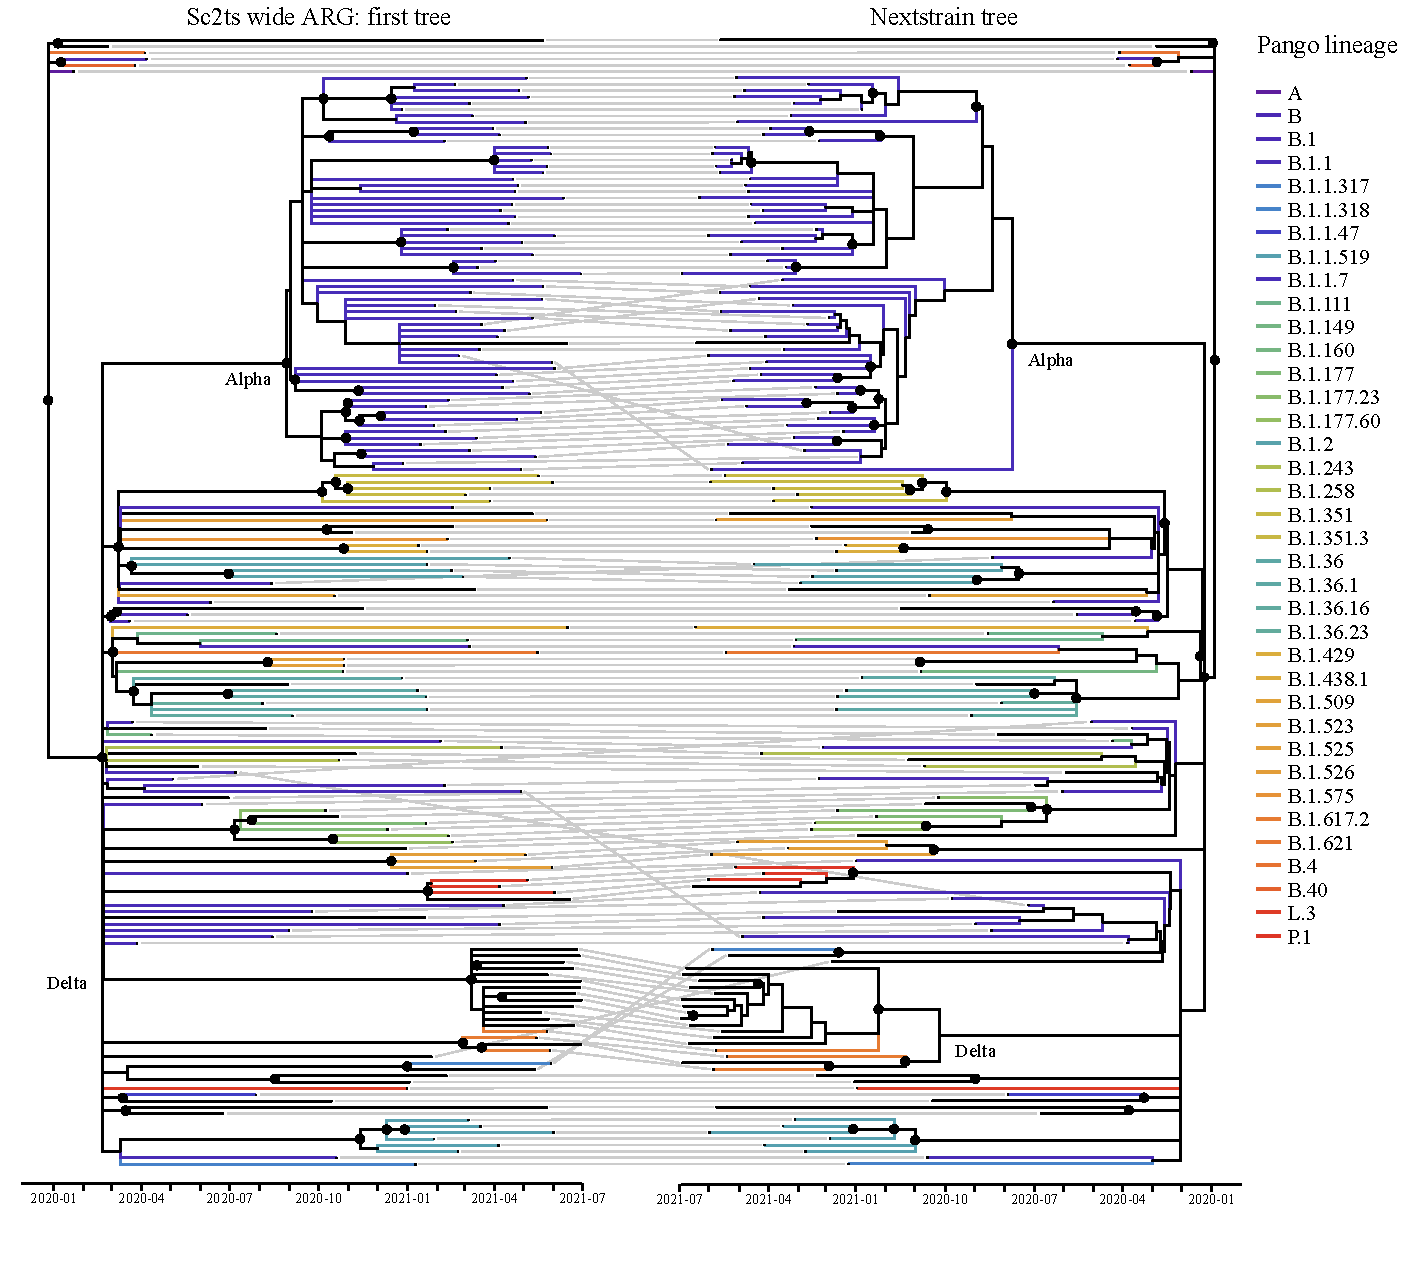
\includegraphics[width=\textwidth]{figures/cophylogeny_wide.pdf}
\caption{\label{fig:cophylogeny}
Tanglegram comparing a local tree from the Wide ARG
(sampled to mid-2021) and an ``all-time'' global Nextstrain tree
(downloaded on January 21, 2023).
Phylogenies are pruned down to those samples present as tips in both datasets. Light grey
lines match the corresponding samples between the two trees; black circles
indicate identical sample partitions between the two trees. Terminal branches
are colour-coded according to the Pango lineage status assigned to the tip
samples; no Pango recombinants are shown, as none are shared between the trees.
The tanglegram was generated using the Neighbor-Net algorithm
\citep{Scornavacca2011-mg} implemented in Dendroscope version 3.8.5
\citep{Huson2012-ys}. See Figure~\ref{fig:cophylogeny_long} for the equivalent
cophylogeny for the Long ARG.}
\end{figure}

A classic tree-based summary of SARS-CoV-2 ancestry is provided
by the Nextstrain project \citep{Hadfield2018-ef}. The trees
available from Nextstrain are based on small subsamples of the
dataset, and early in the pandemic tend to be restricted to
a sample of strains which are not thought to be recombinants.
For validation purposes, we compare our ARGs with
a downloaded Nextstrain tree, restricted to the time period
covered by each ARG. To enable this, we ``simplify''~\citep{Kelleher2018-xc}
the \texttt{sc2ts} ARGs to a backbone containing only those samples
present in the Nextstrain tree. This results in a small set of shared
samples (180 for the Wide ARG, 88 for the Long ARG), none of which are
assigned to Pango recombinant lineages by Nextclade (see Section
\ref{sec:pango_x_lineages}).

The \texttt{sc2ts} backbone phylogenies contain small amounts of recombination,
with 7 recombination nodes in the Wide ARG backbone (8 for the Long ARG
backbone). However, the backbones are highly tree-like, as these
recombination events involve minor, local topological rearrangements
where recombination only occurs between close relatives.
% sometimes even within a single lineage such that the parent
% lineages above a recombination event coalesce with each other before involvement with
% any other part of the phylogeny.
These local reticulations could either represent
real but previously unobserved recombination events between closely related strains,
or could be artefacts of the current \texttt{sc2ts} method and its parameterization.

Figure~\ref{fig:cophylogeny} compares the backbone phylogeny of the Wide ARG with
a GISAID global ``all-time'' tree from Nextstrain
% We give the date below in the caption - we could probably remove if either from there
% or from here (I suggest from here)
(downloaded on January 21, 2023).
We illustrate the backbone phylogeny by visualizing
a single tree in the middle of the viral genome
since other regions of the
genome show almost identical topologies.
It is clear that the backbone topology of the \texttt{sc2ts} tree shows very close
agreement with the Nextstrain tree. The sample genomes cluster by their
assigned Pango lineage status, and many variants and their descendants form
identical monophyletic clades in both the trees (e.g., the Alpha and Delta VoC
clades, labelled).
Supplementary Figure~\ref{fig:cophylogeny_long} shows the same comparison for the Long ARG, with similar results.

Figure~\ref{fig:cophylogeny} also reveals some notable differences between the
trees. Firstly, the \texttt{sc2ts} tree is generally less well resolved,
particularly in early 2020 when sampling density was much lower than
later in the pandemic.
Secondly, there are non-identical sample partitions
near the tips (e.g. within the Alpha clade).
Finally, and most noticeably, some branch lengths differ substantially.
As discussed in Section~\ref{sec:node_dating}, the dating of nodes
other than samples in \texttt{sc2ts} is currently quite crude, and
it is likely that branches not ``anchored'' by samples will be
poorly calibrated. See [SOMEWHERE ELSE] for a discussion of how
these issues may be alleviated in future versions of \texttt{sc2ts}.

\subsection{Mutational spectrum}
\label{sec:mutation_spectrum}
The ARGs inferred by \texttt{sc2ts} and represented using the \texttt{tskit}
library (Section~\ref{sec:args}) are a joint estimate of the processes
of genetic inheritance, recombination and mutation. Unlike most approaches to
phylogenetic analysis, mutations are included in the \texttt{tskit}
data model alongside
the topological representation of genetic inheritance.
This has many
advantages, for example allowing us to compute statistics of the observed
sequences efficiently~\citep{Kelleher2016-wk,Ralph2020-efficiently} and
to provide high levels of data compression~\citep{Kelleher2019-ba}.
The same idea has recently been used to represent
SARS-CoV-2 data in UShER's ``mutation annotated tree''
format~\citep{Turakhia2021-ur}.

\begin{figure} \centering
\newcolumntype{Y}{>{\centering\arraybackslash}X}
\begin{tabularx}{\textwidth}{Yc}

\begin{tabular}[b]{llrlr}\toprule
            & \multicolumn{2}{l}{Wide ARG} & \multicolumn{2}{l}{Long ARG} \\
% \midrule
    \cmidrule{2-5}
Total      & \multicolumn{2}{l}{1,213,193} & \multicolumn{2}{l}{1,062,072} \\
Private     & 758,903 & (62.55\%) &  767,111 & (72.23\%)\\
    \cmidrule{2-5}
Transitions & 873,487   & (72.00\%) & 783,773  & (73.80\%) \\
Transversions & 326,053 & (26.88\%) & 270,333  & (25.45\%) \\
    \cmidrule{2-5}
Insertions  & 6191  & (0.51\%) & 2814   & (0.26\%) \\
Deletions   & 7462  & (0.62\%) & 5152   & (0.49\%) \\
    \cmidrule{2-5}
Recurrent   & 74,719 & (6.16\%) & 50,099 & (4.72\%) \\
Reversions  & 72,617 & (5.99\%) & 48,226 & (4.54\%) \\
\bottomrule
\end{tabular}
&
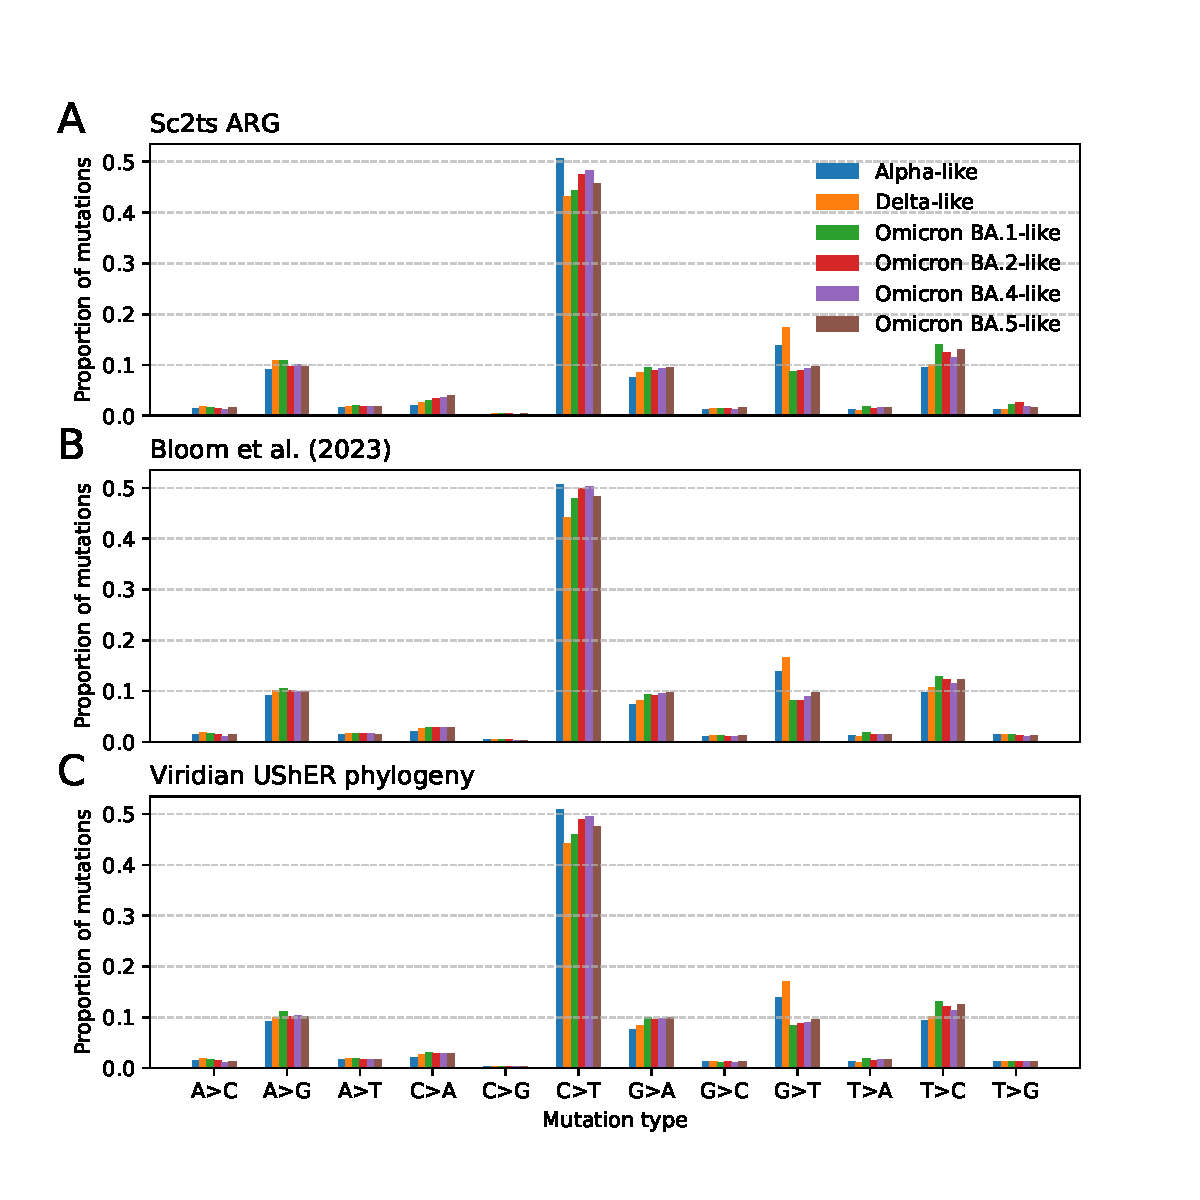
\includegraphics[width=0.35\textwidth]{figures/mutational_spectra.pdf}\\
(A) & (B)\\
\end{tabularx}
\caption{\label{fig:mutational_spectra}
(A) Summary of mutations in the Long and Wide ARGs. Private mutations
occur on terminal branches. Insertions are mutations in which the
inherited state is the gap state ``-'' and the derived state is a
nucleotide, and vice versa for deletions. Recurrent mutations are
those that inherit from at least one other mutation (at that site),
and a reversion is a recurrent mutation that reverses the state change
of the mutation immediately ancestral to it.
(B) Mutational spectrum in
the Wide ARG compared to \cite{Yi2021-sc}. Mutations are
categorised by type (i.e., inherited state $>$ derived state). The percentages
of each mutation type from the Wide ARG are represented by blue bars and the
percentages from Yi et al. by orange bars, with the darker colours representing
one direction (e.g., C$>$U) and the lighter colours the reverse (e.g., U$>$C).}
\end{figure}

The properties of the mutations inferred in the Wide and Long
ARGs are summarised in Figure~\ref{fig:mutational_spectra}A. In both
cases we have a large number of mutations, and a majority of these
(Wide ARG: 62.55\%, Long ARG: 72.23\%) are private to a single
sample, i.e.\ on terminal branches.
Although the average number
of mutations per sample is small
(Wide ARG: 0.77, Long ARG: 1.38; c.f.\ Table~\ref{tab:args}), the average number per site
is large (Wide ARG: 41.23, Long ARG: 36.10; c.f.\ Table~\ref{tab:args}). This is
partly driven by some highly mutagenic sites (e.g., site 28271 has over 7,000
mutations in the Wide ARG, c.f.\ Figure~\ref{fig:breakpoint-distribution}), which
may be artefactual.
A significant issue with the current version of \texttt{sc2ts} is an excess
of inferred reversion mutations, with 5.99\% of all mutations in the Wide
ARG (Long ARG: 4.54\%) reverting the state change of the immediately
ancestral mutation. The majority of these mutations are likely to be
artefactual, and a key goal of future development is to improve
our parsimony heuristics (Section~\ref{sec:parsimony-heuristics}) to
address this issue.

Despite the presence of some artefactual mutations,
the properties of the mutations inferred by \texttt{sc2ts} largely follow
established results.
In Figure~\ref{fig:mutational_spectra}B we compare the mutational spectrum
in the Wide ARG to the results of \cite{Yi2021-sc},
who reconstructed a SARS-CoV-2 phylogeny of
over 350,000 genomes sampled globally from December 24, 2019, to January 12,
2021, and classified the mutations occurring along the phylogeny.
We categorised all single nucleotide
mutations in the Wide ARG by type (defined by the inherited and derived states),
excluding mutations inherited by only a single sample (which are
more likely to be sequencing errors).
Similarly, we took the data for single nucleotide mutations from
\citet[][\url{https://github.com/ju-lab/SC2_evol_signature}]{Yi2021-sc}, excluding
mutations occurring along terminal branches, and tallied them up by type.
Figure~\ref{fig:mutational_spectra}B shows that the mutational spectrum from the
Wide ARG (based on 448,825 mutations) matches that reported by \citet[based on
92,344 mutations]{Yi2021-sc}. In both spectra, C-to-U mutations and G-to-U
mutations occur more frequently than U-to-C and U-to-G, respectively. Similar
results are obtained when including the mutations inherited by only a single
sample or those occurring on terminal branches (data not shown).

\subsection{Early recombinants}
\label{sec:jackson_recombs}
% FIXME: this is rubbish, can someone do better?
RNA viruses are known to recombine at high rates
\citep{Simon2011-rna}, and recombination has been widely
documented to be commonplace in animal and human coronaviruses
\citep{Su2016-epidemiology}. While recombination in SARS-CoV-2
was shown early on to be frequent \emph{in-vitro}
\citep{Gribble2021-coronavirus}, the relatively slow accumulation
of genetic diversity early on in the pandemic hampered efforts to
detect recombinant strains. A number of early studies relying on
analysing patterns of linkage disequilibrium and searching for
mosaic genomes carrying characteristic mutations of different
lineages either failed to detect recombination or posited
that this occurred at low rates \citep[e.g.~][]{Nie2020-phylogenetic,Tang2020-origin,VanInsberghe2021-eu,Varabyou2021-rw}.
The first clear evidence of recombinant lineages was presented by
\citet{Jackson2021-ik}, who performed a careful analysis of sequences
circulating in the UK in late 2020 to early 2021, and found
evidence of multiple independent recombination events and onward
transmission.
By searching for samples combining genomic segments from Alpha (B.1.1.7) and
from the parental lineage B.1.1 based on a list of 22 Alpha-defining mutations,
they found 16 recombinant sequences from 8 putative
origins (groups A to D and four singletons).
These findings are closely replicated in both the Wide and Long ARGs.

\begin{table} \centering
\begin{tabular}{lllll}
\toprule
Group        & Sequences & Method & Interval & Parents \\
\midrule
A (XA)       & 4   & Jackson        &  21,256--21,613 & B.1.177/B.1.1.7 \\
             &     &\texttt{sc2ts} &  21,256--22,228 & B.1.177.18/B.1.1.7 \\
\cmidrule{3-5}
B            & 2   & Jackson        &  6,529--6,954 & B.1.36/B.1.1.7  \\
             &     &\texttt{sc2ts} &  6,529--6,955 & B.1.36/B.1.1.7  \\
\cmidrule{3-5}
C            & 3   &Jackson        &  25,997--27,441 &  B.1.1.7/B.1.221 \\
             &     & \texttt{sc2ts} &  25,997--27,973 &  B.1.1.7/B.1.221 \\
\cmidrule{3-5}
D            & 3   & Jackson        &  21,576--23,063 &  B.1.36.17/B.1.1.7 \\
             &     & \texttt{sc2ts} &  22,445--23,064 &  B.1.36.39/B.1.1.7 \\
\bottomrule
\end{tabular}
\caption{\label{tab:jackson}Comparison of recombination breakpoint
intervals and parent lineages for Groups A-D
reported by \cite{Jackson2021-ik} with the corresponding
recombination events in the Wide ARG.
The second column gives the number of sequences in the group.
Intervals are half-closed, so that for an interval $\ell$--$r$
the breakpoint $x$ can be $\ell \leq x < r$.
Details for all 16 sequences are
given in Table~\ref{tab:jackson_supplement}.}
\end{table}

The Wide ARG contains 15 of these 16 recombinant sequences
(sample MILK-103C712 was removed during preprocessing; see
Section~\ref{sec:data_preprocessing}), and the results are summarised
in Tables~\ref{tab:jackson} and \ref{tab:jackson_supplement}.
Table~\ref{tab:jackson} shows the groups of sequences identified by Jackson
et al.\ as likely independent recombination events with onward transmission.
In each case we have a corresponding recombination node in the Wide ARG,
from which all the sequences in the group descend. The parent lineages
and breakpoint intervals agree closely (see
Section~\ref{sec:breakpoint_intervals} for more details on breakpoint
intervals).
For groups B, C and D,
these recombination nodes form clades consisting only of the identified
sequences.
Group A sequences were subsequently given the Pango XA designation
following onward transmission,
and there are 44 XA designated samples in the Wide ARG (including the
4 sequences analysed by Jackson et al.). The Group A recombination
node forms a monophyletic clade of these 44 samples.
Table~\ref{tab:jackson_supplement} shows the details for each of the
16 sequences individually, and showing generally a strong concordance
in mosaic structure and parent lineages
(including sample CAMC-CB7AB3, which is inferred to have two breakpoints under both
methods).

The Long ARG contains 5 of the sequences: two each from groups A and B
and sample QEUH-1067DEF. These cluster under three recombination nodes, as expected,
and have identical breakpoint intervals and parental lineage assignments
to those of Wide ARG.
The recombination nodes for Group B and sample QEUH-1067DEF are ancestral only
to the sequences involved.
The recombination node for group A forms a monophyletic clade of all
5 XA samples present in the Long ARG
(Figure~\ref{fig:pango-simple-origin-graph}A)

\subsection{Recombination breakpoint intervals}
\label{sec:breakpoint_intervals}
It is rarely possible to be precise about the position on the genome at which
a recombinant sequence switches from inheriting from one parent to another.
Even if we observe the recombinant sequence before signficant
divergence occurs (during onward transmission), if the two parent sequences
are similar there is no way to
% distinguish them.
accurately specify the breakpoint.
Here we define the
interval around a particular breakpoint as the genome coordinates over which the
sequences for the left and right parent nodes are identical. The right-hand
extreme of the breakpoint interval is chosen by the LS HMM Viterbi algorithm
(Section~\ref{sec:ls}), and the left endpoint is then derived by directly
comparing the parent sequences.

\begin{figure}
\centering
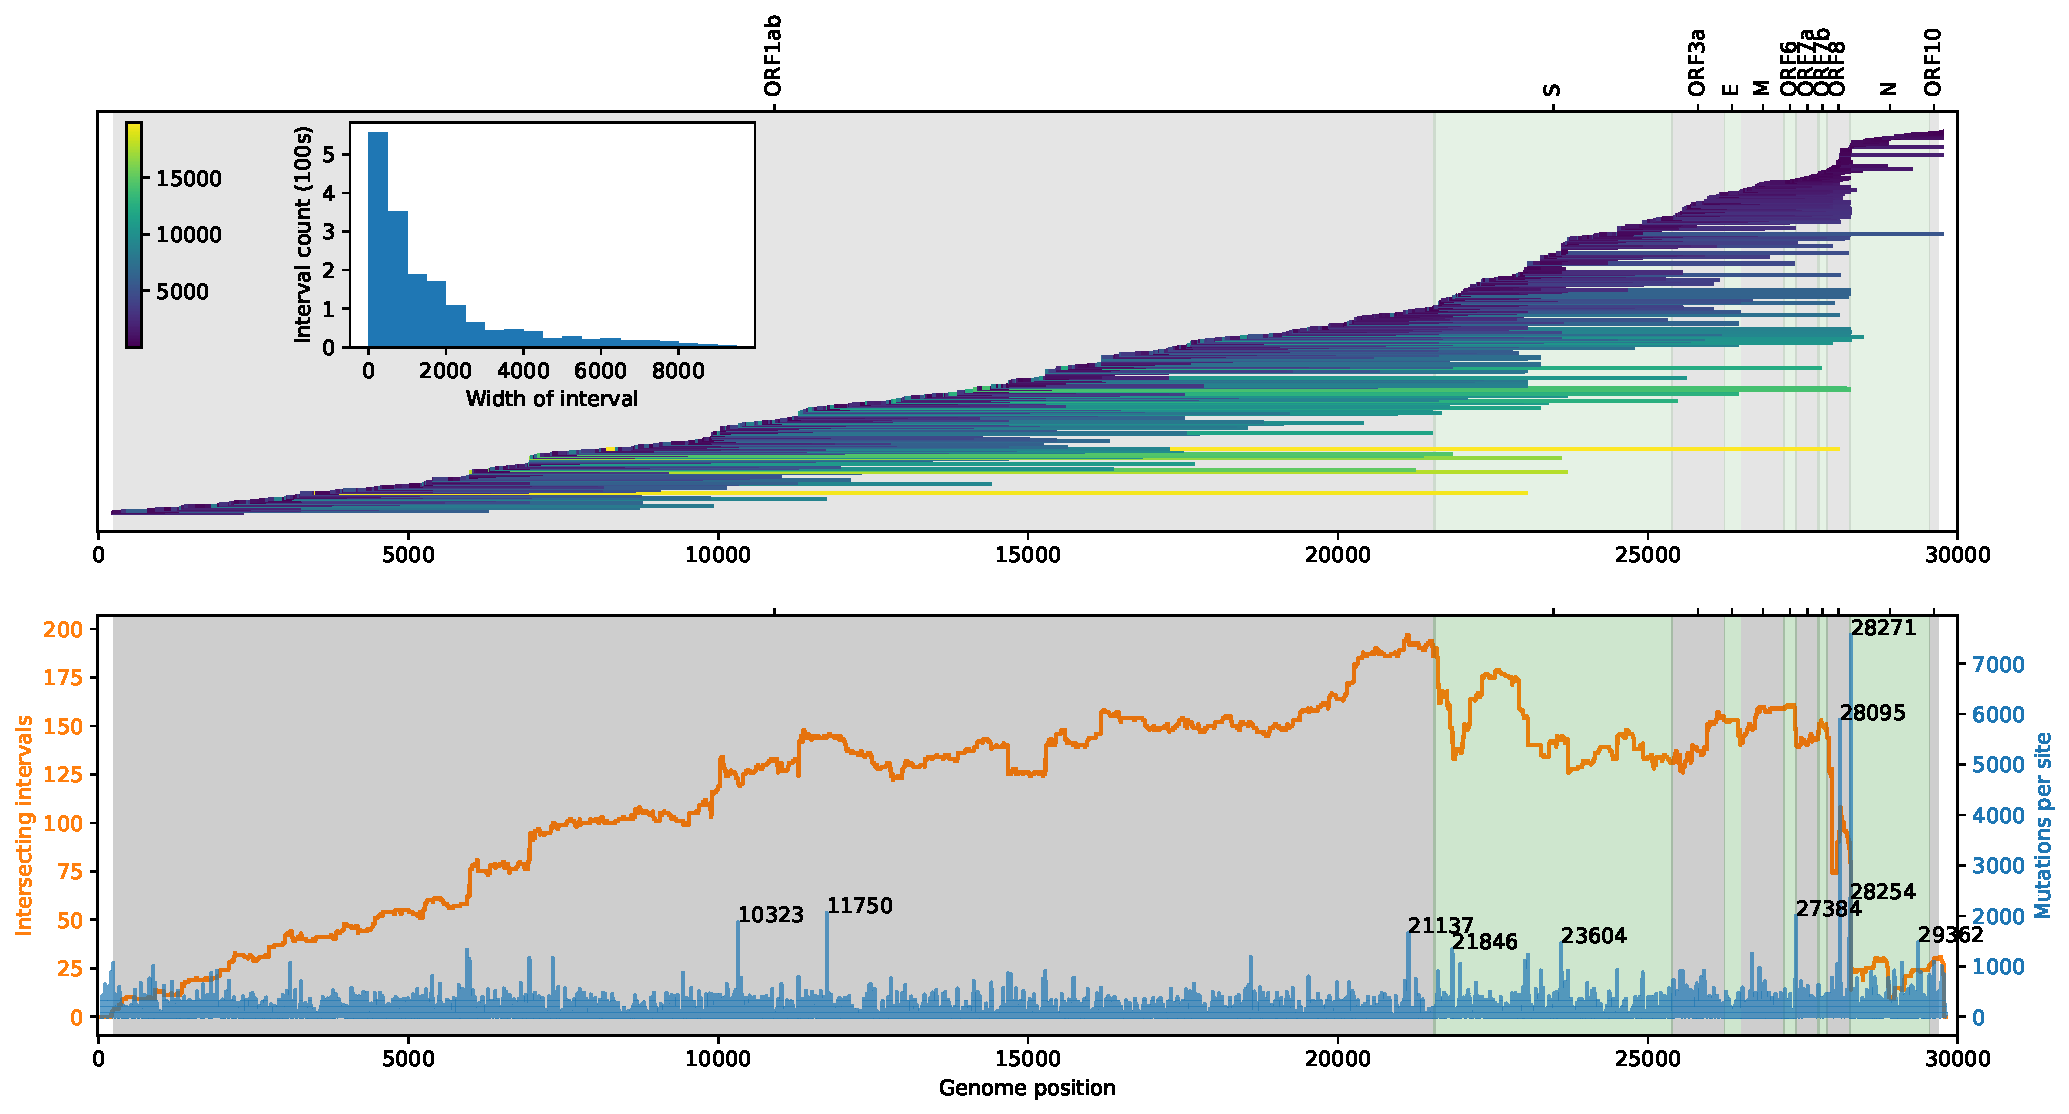
\includegraphics[width=\textwidth]{figures/wide_arg_recombination_intervals.pdf}
\caption{\label{fig:breakpoint-distribution}
Distribution of recombination breakpoints and mutations along the genome in
the Wide ARG. Top panel shows the intervals for 1,769 breakpoints associated
with 1,522 recombination nodes with at least two descending samples, plotted along the genome
as line segments (coloured by interval width). The inset histogram shows the
distribution of these interval widths (truncated at 10kb).
The bottom panel shows the number of intervals that intersect with
each site along the genome (left axis, orange), and the number of mutations
per site (right axis, blue).
The top-ten sites by mutation count are annotated.
See Figure~\ref{fig:long_arg_breakpoint_distribution} for the equivalent plot
for the Long ARG.}
\end{figure}

Figure~\ref{fig:breakpoint-distribution} shows the distribution of breakpoint
intervals and patterns of recurrent mutation along the genome in the Wide ARG
(see Figure~\ref{fig:long_arg_breakpoint_distribution} for the same information
of the Long ARG). We focus on the Wide ARG here as it covers roughly the same time
period as the analyses of \cite{Turakhia2022-it}, facilitating comparisons
of the results. To reduce the effect of artefactual recombinants, we
consider only the breakpoints associated with the 1,522 recombination nodes
that are ancestral to more than one sample. The mean length of these intervals
is 1,685 bases (median 962), and the length distribution is summarised in the
inset histogram in Figure~\ref{fig:breakpoint-distribution}.

Emphasising that further work is required to filter out spuriously inferred
recombination events and improve the accuracy of the inferred breakpoint
intervals, we can draw two preliminary conclusions from
Figure~\ref{fig:breakpoint-distribution}.
% While the detailed interpretation of Figure~\ref{fig:breakpoint-distribution}
% requires further study, a few key properties stand out.[TODO, write this
% better. ]
Firstly, in several cases there is a clear relationship between
gene boundaries and the breakpoint intervals. For example, ORF7a and OR7b
show sharp differences in the number of intersecting intervals within
these genes. This could be due to a number of factors, such as [BIOLOGY]
or the presence of sites with artefactually high numbers of mutations
in the intergenic regions (see the next paragraph for more discussion).
Secondly, we see substantially fewer intervals intersecting with the N
gene than other regions, in agreement with the results of
\cite{Turakhia2022-it}.

It is important to note that the precise endpoints of intervals can be
somewhat arbitrary, since they are defined by exact comparisons
of a recombinant's parents.
% The presence of problematic sites that are enriched
% for errors will therefore tend to artificially truncate breakpoint intervals
% at these sites.
% It is therefore helpful to compare the number of interecting intervals
% with the number of mutations per site in Figure~\ref{fig:breakpoint-distribution}.
% For example, position 28,271 (located in the ORF8-N intergenic
% region) has the largest number of mutations and corresponds to the
% left endpoint of 9 intervals and the right of 57.
% The 7,572 mutations  (including 5,782 insertions and 1,605 deletions)
% at this site are a likely indicator that this
% homopolymeric region is prone to sequencing errors
% and should be included in the list of ``problematic sites'' that
% are excluded from analysis (Section~\ref{sec:data_preprocessing}).
% There can be good biological reasons for this too though
% However, hypermutable sites such as 27,972 \citep{Jungreis2021-dh}
% have the same effect of truncating intervals. At this site we have
% 770 mutations (including 425 C$>$T, 314 T$>$C) with potential signals
% of polymorphism maintained by selection [FIXME!!], and 58 intervals
% with endpoints within one base of this site.
Thus, breakpoint intervals will tend to be truncated at sites which are
hypermutable, either due to being prone to sequencing errors or
for biological reasons such as selection pressure.
It is therefore helpful to compare the number of intersecting intervals
with the number of mutations per site in Figure~\ref{fig:breakpoint-distribution}.
For instance, position 28,271 (located in the ORF8-N intergenic
region) has the largest number of mutations and appears as an endpoint
of 66 intervals.
The 7,572 mutations (including 5,782 insertions and 1,605 deletions)
at this site are an indicator that this
homopolymeric region may be prone to sequencing errors
and should be included in the list of ``problematic sites'' that
are excluded from analysis (Section~\ref{sec:data_preprocessing}).
On the other hand, 58 of the breakpoint intervals have endpoints
within one base of site 27,972, which has undergone 770 mutation events
(including 425 C$>$T, 314 T$>$C). The C$>$T mutation has the effect of
truncating ORF8, and it has been posited that the truncation is neutral
or advantageous for transmission, and disadvantageous within-host
\citep{Jungreis2021-dh}, suggesting that the high rate of recurrent mutation
at this site is due to selection.

% JK Dropping this for now:
% We further consider the breakpoint intervals within the context of
% recombination breakpoint sequence motifs. It is hypothesised that certain
% palindromic breakpoint sequences (specifically, CAGAC and CAGAT) promote
% template switching during replication in SARS-CoV-2 via formation of
% base-paired stem loops in the genome structure \citep{Gallaher2020-lb}. There
% are 87 occurrences of these two breakpoint sequences in the Wuhan-Hu-1/2019
% reference sequence (Supplementary Table 5). We observe that XX (XX\%) of the
% breakpoint intervals of the HMM-consistent recombinants span at least one of
% the breakpoint sequences.

\subsection{Divergence between recombinant parents}
\label{sec:parent_divergence}
% Paragraph 1, what does all this mean?

% Purpose of this paragraph - remind the reader that we can only do this
% sort of things because we have an ARG, and we can do  this at a far
% greater level of granularity than existing methods.
[ FIXME this is a rough outline of what an intro para might say]
An important advantage of inferring a joint model of inheritance,
mutation and recombination in an ARG (Section~\ref{sec:args})
is that this allows us to precisely trace the origins of recombinants.
[Katherine - need some input from you here to say this properly?]
Existing methods only provide us with approximate estimates of
the origins of recombination events, and are not able to distinguish
recombinations between closely related lineages.

% Paragraph 2, what do we plot, specifically?
In this section we investigate the patterns of divergence between
the parents of recombination nodes.
We focus on the Long ARG because it covers time
periods where recombination is known to have occurred
a large number of times, for example it contains samples from over
30 Pango X lineages (i.e., those inferred
to have recombinant ancestry; see Section~\ref{sec:pango_x_lineages} for
further analysis of Pango recombinant lineages in the Long and Wide ARGs).
Figure~\ref{fig:recomb_mrcas} shows the estimated date of the most recent
common ancestor (MRCA) of the parent nodes for each recombination breakpoint,
plotted against the divergence between these parents (i.e. the
total branch length from the parents to their MRCA in the trees to
the immediate left and right of the breakpoint).
As in Section~\ref{sec:breakpoint_intervals}, in these plots we
exclude breakpoints associated with ``singleton'' recombination nodes
(those ancestral to only one sample).
Larger points distinguish those breakpoints which occur in nodes
ancestral to 5 or more samples, comprising 316 breakpoints from
291 recombination nodes. The criterion of 5 descendants matches the
minimum number required to designate a new Pango recombinant lineage
\citep{Rambaut2020-dw}, and serves to highlight those recombinants which
have greater epidemiological significance.

% that we deem to be more reliable by the measure of ``HMM consistency''.
% We define an  in that when we compare the LS HMM results when run from
% 5' to 3' versus 3' to 5', it gives the
% same mutations patterns and sequence-identical 5' parents as when run 3' to 5'
Note that as each plotted point represents a breakpoint, a recombination
node with more than one breakpoint (e.g. with 3 or more parents,
comprising ${\sim}10 \%$ of the
recombination nodes in Figure ~\ref{fig:recomb_mrcas}) will be represented by several points.
We caution that some of the time estimates in these figures
come with a substantial degree of uncertainly,
since non-sample nodes are dated somewhat crudely in the current version
of \texttt{sc2ts} (Section~\ref{sec:node_dating}). Nevertheless, the histograms
clearly show that \texttt{sc2ts} can identify recombination between lineages
that are only a few weeks apart.

\begin{figure} \centering
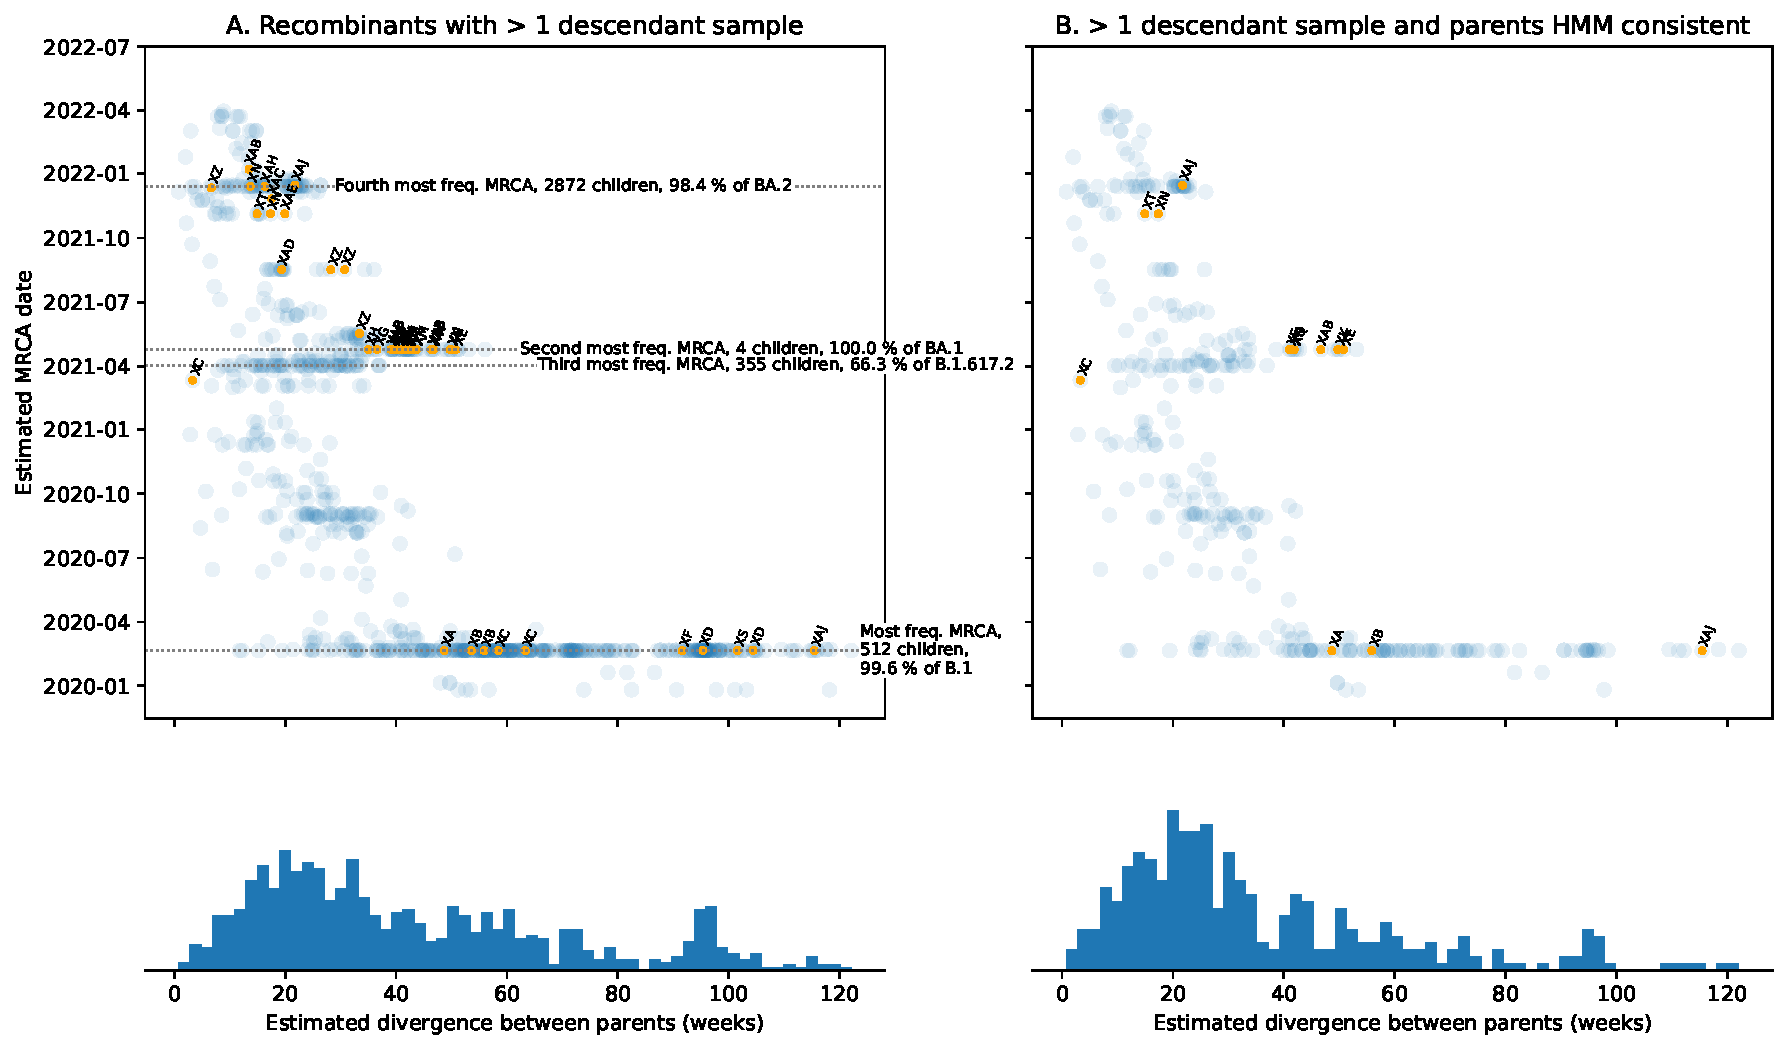
\includegraphics[width=\textwidth]{figures/recombination_node_mrcas.pdf}
\caption{\label{fig:recomb_mrcas}
Date of common ancestry between the parents on either side of recombination
breakpoints, as a function of the divergence time between the parents.
MRCAs of parents associated with Pango designated recombinants (XA, etc)
are identified in orange. Larger symbols represent breakpoints in recombination
nodes which are ancestral to five or more samples.
Horizontal dotted lines show the four most common MRCA nodes,
which tend to be associated with major outbreaks and with many immediate children.
The stacked histogram shows the distribution of parental divergence times, ranging
from parents that have diverged only a handful of days previously, to much more
divergent parent lineages. See Figure~\ref{fig:recomb_mrcas_voc_breakdown}
for equivalent plots broken down by parental VoC classification.
}
\end{figure}

% Paragraph 3, what do we say about the dates/nodes of the MRCAs?
The date of the MRCA of recombinant parents is
concentrated in several banded rows in Figure~\ref{fig:recomb_mrcas}. These are
largely due to a few MRCAs shared by many
recombinants; the top four are indicated by dotted lines in the
figure. These shared MRCAs lie near the root of large expansions
(B.1: original variant, B.1.617.2: Delta, BA.1: first Omicron wave,
and BA.2: second Omicron wave), as demonstrated by the number of samples with those
Pango designations which trace back to each ancestral node (listed as
percentages on the plot). The majority of these frequently-shared MRCAs
are associated with large polytomies (at the extreme,
the BA.2-linked node has 2,872 immediate children), likely
indicating a rapid and under-sampled expansion of a clade.

% Paragraph 4, what do we say about the divergence times?
The histograms in Figure~\ref{fig:recomb_mrcas} show that there is a
broad range in divergence times among recombinant parents.
We can also see that the majority of recombinants arise
from parents that diverged 10 to 30 weeks
previously. However, there is also a peak of recombinants that diverged
${\sim}95$ weeks prior to the event: these correspond to recombinants whose
parental common ancestor traces to early 2020. We would expect, for example
Delta-Omicron recombinants to fall into this group, hence it can be
useful to classify the breakpoints further by the VoC combinations of their
parent lineages. Considering only the Alpha, Delta, and Omicron VoC classes,
such a classification reveals that the majority of breakpoints have two Delta or
two Omicron parents, and that Omicron and Delta are the variants associated
with the most recombination (Supplementary Figure~\ref{fig:recomb_mrcas_voc_breakdown}).
This may reflect either sampling intensity, the
prevalence of cases (which increases the
chance of coinfection and recombination), or possible heterogeneity in
recombination probabilities among lineages.

\subsection{Recombinant Pango lineages}
\label{sec:pango_x_lineages}

In this section we focus on the detailed genealogy of samples that have been
previously identified as recombinants, i.e. given a Pango designation that
starts with an ``X''. We focus primarily on the Long ARG in this section,
since it contains many more recombinants; the status
of Pango X lineages in the Wide ARG is briefly summarised in Section~\ref{sec-pango_x_wide_arg}.

The Long ARG contains 749 samples designated by Nextclade [CITE] as Pango
recombinants, classed into 33 Pango lineages; this
reduces to 711 samples from the same 33 lineages
when singleton recombinants (i.e. recombination
nodes subtending only one sample) are removed.
In contrast, using the alternative GISAID designation process [CITE], only
515 samples in the Long ARG are labelled as Pango recombinants,
which fall into 38 lineages (when singleton recombinants are excluded this
drops to 514 samples from 35 lineages). The variation in Nextclade versus
GISAID classifications highlights the frequent uncertainty that exists when
assigning Pango X lineages to samples.

Below we focus on the 749 Nextclade-designated recombinant samples, all
but two of which descend from a recombination node in the Long ARG.
These two samples are designated XP, and a likely
explanation for the absence of a corresponding recombination event in the Long ARG
is that the characteristic multibase deletion for XP
(\url{https://github.com/cov-lineages/pango-designation/issues/481}) is masked
during preprocessing (See~\ref{sec:data_preprocessing} for details and potential
improvements). 38 of the remaining X designated samples are singleton recombinants,
descending
from recombination nodes that are ancestral only to that sample (10 are XZ; 6
are XE;  3 each from XN and XK; 2 each from XC, XS, XV, XQ and XAB; and 1
sample from each of XB, XM, XJ, XAF, XAH and XAJ). Such samples are likely to
be enriched for sequencing errors and lineage designation artefacts, and so we
exclude them from further analysis in this section.

The most recent recombination node for 79 samples (XN: 53, XZ: 16, XAJ: 6, XE:
1, XAD: 1, XAH: 1, XAK: 1) is the same. This node, caused by strain
Denmark/DCGC-281594/2021, is ancestral to more than 127K samples,
and is highly likely to be a spuriously inferred recombination event.
Understanding the origin of this
and other similar high-impact, but likely spurious recombination
events is an important aspect of future work.
For simplicity, we exclude these samples from further analyses in
this section.

The remaining remaining 630 Pango recombinant samples trace back to 50 different
most recent recombination nodes, corresponding to 31
Nextclade-designated Pango lineages. These are summarised
in Supplementary Table~\ref{tab:pango-recombinants}, and fall
into three classes: single origin, multiple origin,
and multiple nested origins, which we discuss in the following sections.

\subsubsection{Single origin}
In the absence of genealogical information, a reasonable initial assumption is
that all sequences
assigned to a given Pango X lineage are descendants of a single recombinant
sequence, arising as a result of a mixed infection followed by onward
transmission. We would expect our ARG to reveal evolutionary histories of this
nature, where all the samples assigned to a given recombinant lineage
trace back to one recombination node, representing a single originating
recombination event. In the Long ARG, 16 of the 31 Pango recombinants lineages identified by Nextclade
fall into this category (Supplementary Table~\ref{tab:pango-recombinants})

\begin{figure}
\centering
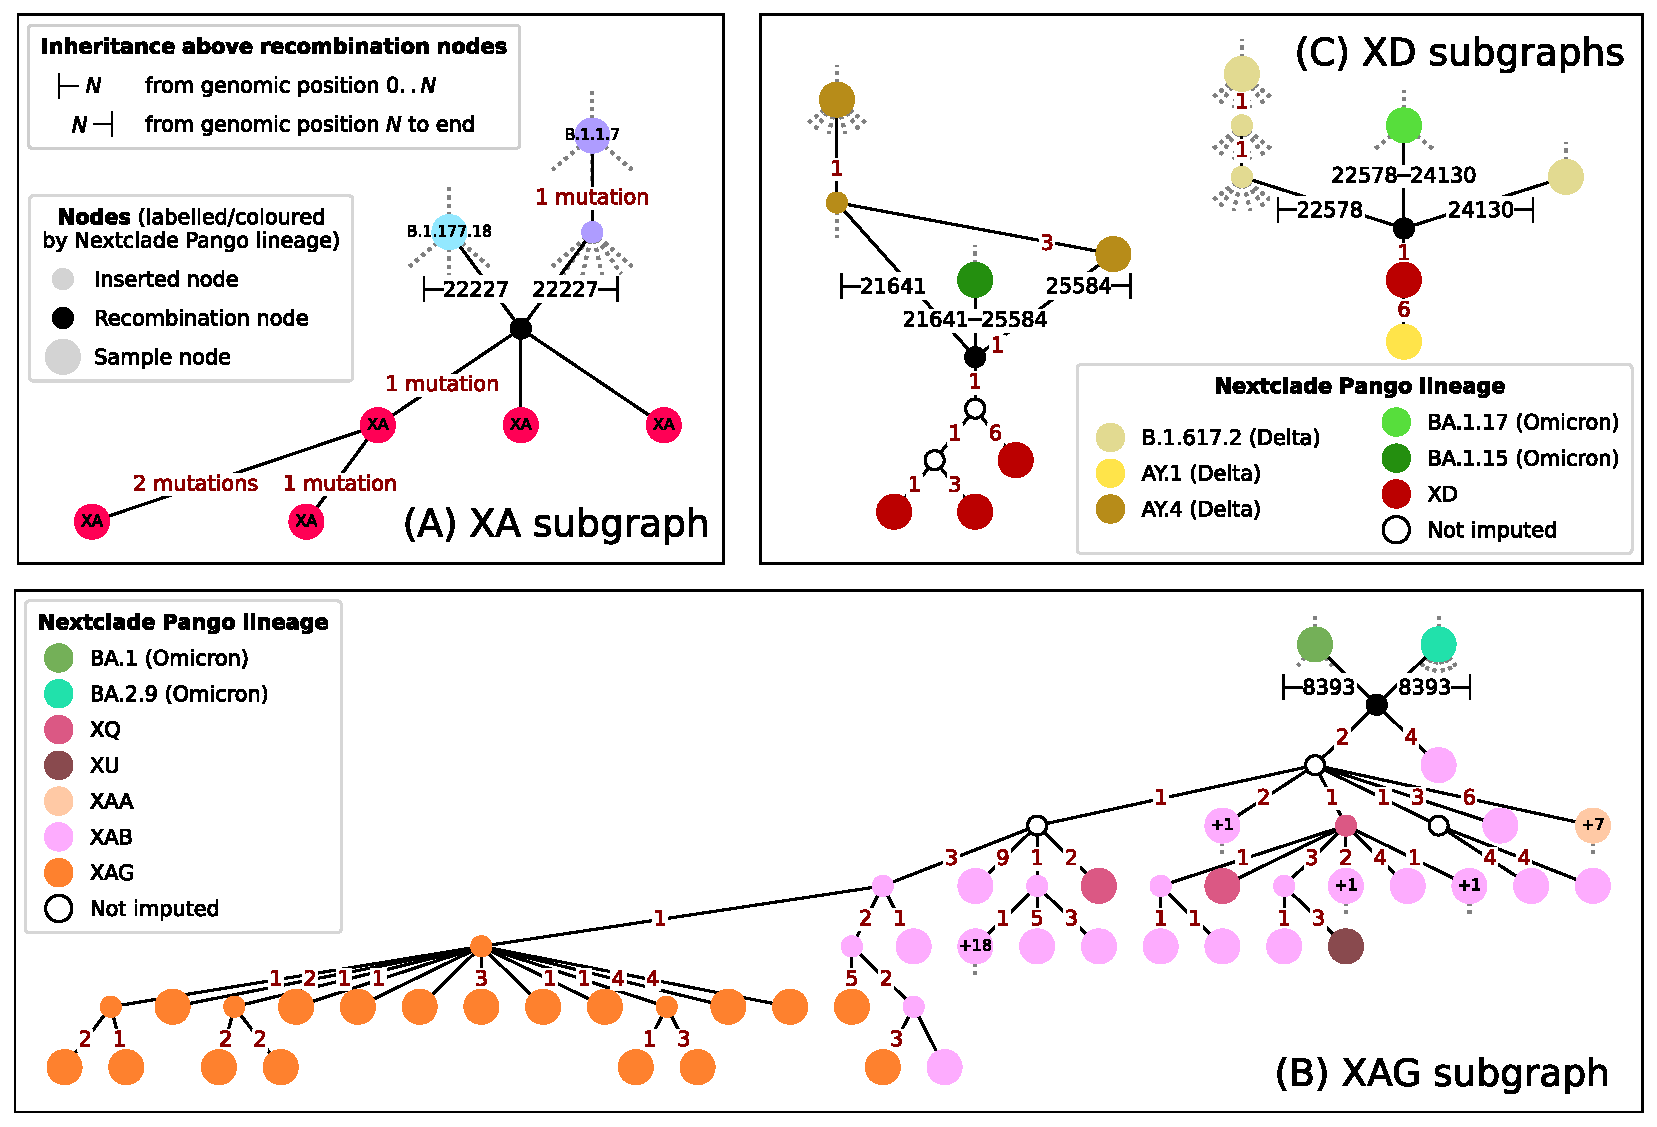
\includegraphics[width=\textwidth]{figures/Pango_XA_XAG_XD_nxcld_tight_graph.pdf}

\caption{\label{fig:pango-simple-origin-graph} Examples of non-nested
Nextclade Pango X lineages. (A) Subgraph for XA in the Long ARG: all five samples designated
as XA by Nextclade, together with their ancestral lineages, are shown outwards to the nearest
sampled viral genome; dotted lines show ARG continuation. Vertical position of nodes does not
show absolute time, but simply relative rank (parents above children). Nodes are coloured by Nextclade
Pango designation; smaller symbols are non-sample nodes inserted by \texttt{sc2ts}, whose
Pango status is imputed. Genomic regions inherited by the recombination node are shown;
breakpoints correspond to the maximum breakpoint position inferred by \texttt{sc2ts}.
(B) Equivalent subgraph for the 17 XAG samples in the Long ARG, with abbreviated labelling. Where
non-XAG samples are ancestral to other samples, the number of descendant samples is marked as ``+1'',
``+7'', etc.
(C) Equivalent subgraphs for both origination events involving the four XD samples in the Long ARG.
Details of the mutations and sample node identities for all three plots are provided in
supplementary Figures \ref{fig:pango_XA_gisaid_graph}, \ref{fig:pango_XAG_gisaid_graph}, and \ref{fig:pango_XD_gisaid_graph}, which also provide alternative GISAID Pango designations.
} \end{figure}

One of the simplest examples is the case of XA, corresponding to group A
of \citet{Jackson2021-ik} as discussed above. Figure~\ref{fig:pango-simple-origin-graph}A
shows the exact relationships inferred by \texttt{sc2ts} as a subgraph of the Long ARG.
Here, paths have been traced from all
Nextclade-identified XA samples (in red) to the closest other sample nodes in the ARG.
Sample nodes are plotted as larger circles, but the subgraph also includes intermediate,
non-sample nodes: i.e. inserted nodes such as UPGMA, recombination, mutation collapse, and
reversion push nodes, plotted as smaller circles. Dotted lines show where this subgraph links
to the rest of the ARG. Above recombination nodes, only ancestral nodes are shown, meaning
that the subgraph is not extended to show additional descendants of recombinant parents.

It is clear from the XA subgraph that all the samples labelled XA by Nextclade trace to a
single originating recombination node, whose genome is a composite of a B.1.177.18 lineage
on the left of the genome and a B.1.1.7 lineage on the right. In the subgraph we show
the maximum genomic position for the recombination breakpoint, here at 22,227 basepairs
(corresponding to a breakpoint strictly less than 22,228, see Table~\ref{tab:jackson})

%% Discuss panel B where XAG shares a common recombinant origin with samples from several other X lineages

A more complex single-origin case is XAG, illustrated in
Figure~\ref{fig:pango-simple-origin-graph}B. Here, the XAG samples
all trace back to the same most recent recombination node
(combining BA.1 on the left and BA.2.9 on the right), but
we infer this recombination event to also be the originating event for
all the recombinant samples designated XAA,
and some, but not all, of those identified as XAB, XQ, and XU by Nextclade.

The classification of originating recombination events is dependent on
accurate designation of Pango lineages to samples. It is therefore important
to note that if the GISAID Pango designations are used, many of the samples
marked here as XAB are reclassified as BA.2 (and XAG becomes fully monophyletic,
see supplementary Figure \ref{fig:pango_XAG_gisaid_graph}). This is an
independent confirmation of the uncertainty in designation of these XAG-related
samples.

Six of the 16 Nextclade designated lineages (XA, XAC, XAE, XF, XK, and XS) are of the
basic (XA) type with no other Pango designations among their descendants.
The remaining ten are of the XAG type with multiple Pango
designated lineages as additional descendants of the originating recombination event.
In some cases,
these may be, however, be a result of erroneous Pango designations.
Supplementary Table~\ref{tab:pango-recombinants} also shows the official
Pango designated parent lineages and \texttt{sc2ts} inferred parent lineages,
which extensively agree (although \texttt{sc2ts} provides more a precise
parent designation).

\subsubsection{Independent multiple origins}
The \texttt{sc2ts} inference process has no pre-defined knowledge
of Pango X lineage assignments, and there is therefore no particular
requirement that all the samples assigned to a given lineage must trace back to
a single recombination event. Using Nextclade-designations, 15 Pango X lineages are
inferred to have multiple
recombinant origins, such that their samples trace to $>$1 most recent
recombination node in the ARG. Of these, 11 are cases where the
recombinants are independent rather than nested (i.e. there is no overlap in the list
of descendant samples for each recombination node). Most have a single ``main''
recombination event from which the majority of the corresponding recombinant samples
descend, and which agrees with the offical Pango designated parent lineages
(see Supplementary Table~\ref{tab:pango-recombinants}, but note that
in XJ and XU there are too few Pango X samples to decide on a ``main'' clade).

Figure~\ref{fig:pango-simple-origin-graph}C shows a simple multiple-origin example, consisting of
the 4 samples labelled XD by Nextclade in the Long ARG. The left hand subgraph
(the origin of three XD samples, all sampled in France) has an earliest
sample with EPI\_ISL: 11222324 (dated 2022-02-26), while the right hand
subgraph has a single sample with EPI\_ISL~8514045 (sampled in Turkey and dated 2021-12-30).
Both involve an Omicron lineage being inserted into the middle of a Delta genome, but
the breakpoints in each case are slightly different: the start of the Omicron insertion
in the French samples has an estimated maximum position of 21641 basepairs
(and minimum of 21619, not shown) with the insertion end occurring at a maximum position of 25584
(and a minimum of 25470). In contrast, the Omicron insertion in the Turkish sample
is inferred to have occurred between positions 22578 (min 21619) and 24130 (min 23605).
The breakpoint difference, the different geographical locations, the time between the
samples, and the fact that the two samples differ at 23 nucleotide positions,
suggests that these may indeed represent true independent Deltacron recombinants.
The canonical XD definition is based entirely on samples from northern Europe, particularly
France (\url{https://github.com/cov-lineages/pango-designation/issues/444}) so it seems
plausible that the earlier Turkish sample has been mislabelled XD by Nextclade.
Indeed, GISAID does not label any of these samples XD (see Supplementary
Figure~\ref{fig:pango_XD_gisaid_graph} which gives exact mutations and sample identifiers).
Investigation of other multiple-origin examples reveals somewhat similar patterns,
suggesting that most of the simple multiple origin examples are due to incorrect
Pango labelling.

\subsubsection{Nested recombinant origins}
As well as cases where Pango X lineage origins are attributed to independent
recombination events, four Pango X lineages in the Long ARG have Nextclade-designated
samples whose ancestry involves multiple non-independent (``nested'') recombination events
(marked by~\textdagger ~in Supplementary Table~\ref{tab:pango-recombinants}; the most
complex appears to be XAB). Figure~\ref{fig:complex_origins_graph} plots the earliest example,
XB,  which is present in both the Wide and Long ARGs. The subgraph shows a recombination
between a B.1 sample and B.1.627 sample that leads not only to all the XB-labelled samples
but also to a ``hairball'' of further recombination nodes whose descendants are often not
identified as recombinants by Nextclade (plotted on the left, in blue). A similar
pattern is seen when examining XB in the Wide ARG (see discussion below).

\begin{figure} \centering
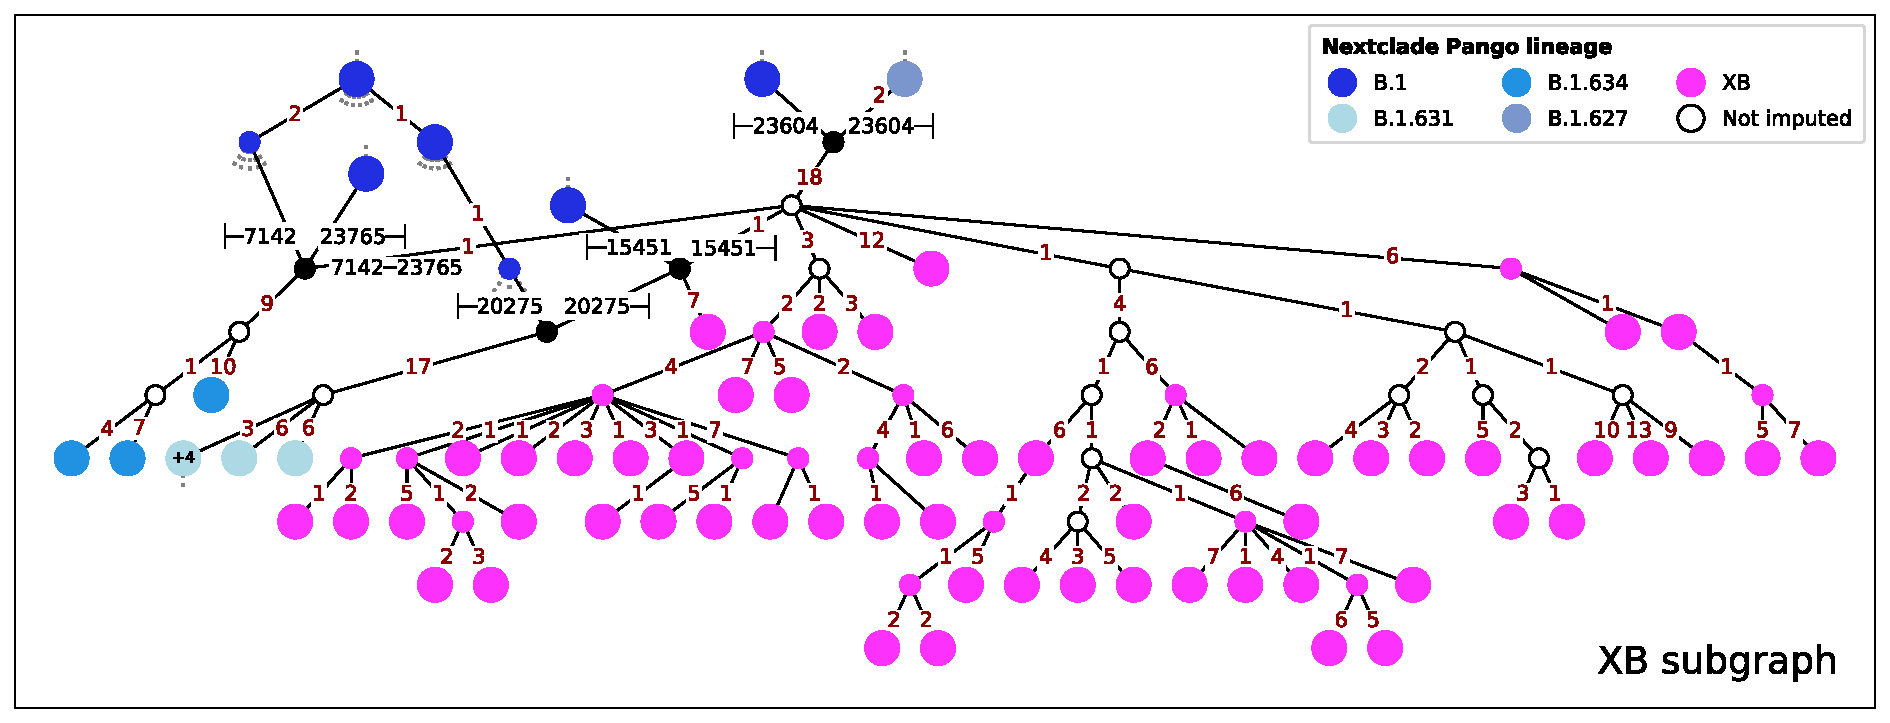
\includegraphics[width=\textwidth]{figures/Pango_XB_nxcld_tight_graph.pdf}
\caption{\label{fig:complex_origins_graph}  A subgraph of the Long ARG showing
nested recombination events involving Pango lineage XB. All XB samples
trace to a single recombination node (top centre), but three further recombinations
also descend from this node. The samples descending from these nested
recombinations include 9 that are assigned by Nextclade to
various non-recombinant pre-Alpha lineages (blue).}
\end{figure}

Note that in the Long ARG, the nested recombination events account for only one
XB sample (pink upper left, with 7 mutations above it); moreover, this sample is
not identified as XB by GISAID (Supplementary Figure~\ref{fig:pango_XB_gisaid_graph})
indicating some uncertainty in lineage assignment in this part of the ARG.
Also note that the number of mutations on the lineages immediately above and
below the recombination node (totalling 18+2) is rather large, suggesting
that the sampled recombinant which induced the recombination node in the Long ARG
is only distantly related to the true originating recombinant. This could account
for complex and potentially artefactual relationships around these nodes, and
is likely to be due to undersampling of the XB outbreak. Investigating examples
of nested recombinant origins, and identifying which (if any) of the nested
recombination events may be artefactual, is an important area of future research.

\subsubsection{Wide ARG}
\label{sec-pango_x_wide_arg}
%% Quick overview of the wide ARG.
Since the Wide ARG is restricted to data collected prior
to mid-2021, it contains samples from only three Pango-designated recombinant
lineages: XA, XB, and XC. Both Nextclade and GISAID designate 44
samples as XA, while 237 samples are designated
as XB by Nextclade (231 by GISAID), and 6 as XC by Nextclade (none by GISAID).
After removing singleton recombinants, XA numbers remain unchanged, but XB is
reduced to 235 Nextclade-designated samples (229 GISAID) and XC is reduced to 4
(none in the GISAID designations). We correctly identify that all samples
designated as XA, XB, or XC by any method have one or more recombination nodes
in their ancestry.

%% Textual description of the 3 recombinant lineages present in the wide ARG
As in the Long ARG, all XA samples in the Wide ARG trace back to a
unique originating recombination node. This is the product of a recombination
between a B.1.177.18 sample (specifically the strain Wales/ALDP-115BF41/2021,
EPI\_ISL: 1012804) which contributed the majority of the genome from the start
to a maximum position of 22227, and an unknown (inserted) node with imputed
Pango lineage B.1.1.7, which contributed the remaining right hand portion. The
recombination node has five immediate children: four sample leaves (EPI\_ISLs:
989697, 1019487, 1104468 and 1122630) and a UPGMA-inserted node which is the
ancestor of all other XA samples in the dataset.

For XB, all samples trace back to an originating node which is the product of a
recombination between a B.1 sample (specifically the strain
England/CAMB-7B47D/2020, EPI\_ISL\_433960, which contributed the majority of
the genome from the start up to a maximum position of 23604bp), and two
UPGMA nodes with imputed Pango lineages B.1.627 (up to a maximum position of
27389bp) and B.1.36.8 (the remaining fragment of the genome). Figure~\ref{fig:complex_origins_graph}
shows that in the Long ARG the equivalent recombination node has only 2 parents,
with no involvement of  B.1.36.8; it is possible that the third parent in
the Wide ARG is artefactual. As in the Long ARG, additional
non-X-designated samples such as B.1.634 also descend from this recombination,
and there are also a small number of nested recombination nodes. However, all but
one of these nested recombinations are unimportant, being ancestral to negligible fractions
of the Nextclade-designated XB samples. The one exception accounts for about 17\% of the
designated XB nodes, and involves a recombination between descendants of the
originating XB recombination. More specifically strain
USA/TX-HMH-MCoV-43092/2021 (EPI\_ISL 2224652) is inferred to be a recombination
between an XB grandparent and its XB grandchild. This could well be
artefactual.

For the few XC-labelled samples, the Wide ARG identifies more than one
originating recombination node. However, as none of the samples designated as
XC by Nextclade are designated as XC by GISAID, these patterns could be due to
mislabelling, and greater number of XC samples would be needed to draw reasonable
conclusions.

% JK: removing this for now

% \subsection{Novel recombinants}
% Next, we examine recombination nodes in the
% Long ARG (sampled to mid-2022) that represent previously unnamed putative
% recombinant sequences, which do not have a Pango recombinant designation. For
% this proof-of-concept study, we have arbitrarily picked 12 recombination nodes
% that seem plausible (Supplementary Table 4). All these nodes involve Omicron
% subvariants (BA.1, BA.2, BA.4, and BA.5). These recombination nodes (1) were
% inserted into the Long ARG on or after January 8, 2022; (2) have at least 10
% descendent samples; and (3) have no mutational differences (including immediate
% reversions) from their parent nodes.

% TODO: Node  740761 (USA/NC-CDC-LC0668306/2022) is a sister clade proposed1006
% in the UShER public phylogeny. Node 628656 (Scotland/QEUH-37794BB/2022) is a
% sister clade of XAC, and annotated as ``miscBA2BA1PostSpike''.

\section{Discussion}
% PARA 1. SARS-CoV-2 is still important, and the vast hordes of data provide an
% unprecedented opportunity to study the evolution of a virus. Even if the
% public health emergency is officially over, it doesn't mean it's not coming
% back and we should be prepared. Recombination is now a vital factor, and
% present a way in which it can be incorporated. Our results are accurate.
Although the COVID-19 pandemic is no longer considered a global emergency
by the WHO, the prevalence of SARS-CoV-2 continues to be high worldwide
with persistent high levels of infection. This high prevalence has allowed the
proliferation of many variants, with more than 600 Pango-designated lineages
circulating globally in the last three months (January to March, 2023;
https://gisaid.org/; access on March 27, 2023). High prevalence also brings a
higher risk of coinfection, increasing opportunities for new phenotypically
distinct recombinants to emerge and spread. Phylogenetic approaches have
been central to pandemic responses thus far [TODO: Examples and citations].
However, as recombinant lineages are now endemic and it is clear that
recombination is a major feature of ongoing SARS-CoV-2 evolution,
it is imperative that these methods are updated to incorporate the
effects of recombination, and future public health interventions are
not based on incomplete and potentially biased evolutionary models.
Here we have introduced the first method to infer an evolutionary
history that jointly models genetic inheritance, mutation and
recombination at pandemic scale, and illustrated how this single
structure accurately captures results derived by many different means.

% PARA 2. Here are things that could be improved in the short term. Here's a
% few more, longer term ideas.
Nonetheless, \texttt{sc2ts} is currently ``alpha'' quality software, and
we caution against overinterpreting current results. As we have sought
to illustrate throughout, there are some clear areas for improvement
and some relatively straightforward changes that could be made to
improve inference. The pipeline used to identify and
mask erroneous sites in the input alignments is simplistic, and, among
other issues, results in multi-base indels being marked as missing data
(Section~\ref{sec:data_preprocessing}). A more sophisticated
approach~\citep[e.g.][]{Aksamentov2021-hj} would
likely yield significant improvements, and reduce the effect of sites with
artefactually high levels of mutation (e.g., site 28271;
Section~\ref{sec:breakpoint_intervals}).
Using a pre-existing tree built using state-of-the-art phylogenetics methods
for the early stages of the pandemic (Section~\ref{sec:backbone_phylogeny}),
and minor adaptations to standard node-dating methods
(Section~\ref{sec:node_dating}) should help resolve the most notable issues with
the inferred backbone phylogeny (Figure~\ref{fig:cophylogeny}).
Trees constructed from daily sample clusters have a surprisingly large
influence on the overall ARG topology
(Section~\ref{sec:sample-cluster-tree-inference}), and so using a more
sophisticated tree building approach should yield clear improvements.
The unrealistically large number of reversion mutations
(Section~\ref{sec:mutation_spectrum}) may be reduced by
improvements to the current parsimony
heuristics (Section~\ref{sec:parsimony-heuristics}).
A major source of errors are the ``time-traveller'' samples, whose
provided collection dates are months (or years) too early
(Section~\ref{sec:filtering_time_travellers}).
% Hmm, not sure about this. Wouldn't this also rule out new major lineages
% also (which tend to show up with a bunch of new mutations?) I guess it
% depends on the threshold, and we could set it according to previous
% experience with new lineages?
While it is unclear how
we might solve this problem in general, some simple solutions such
as filtering out sequences that exceed a given cost in the LS HMM
(i.e., number of mutations and recombination switches) may work well
in practice. Such an approach would also reduce the impact of sequences
with high levels of sequencing error (which contribute a large number of
mutations, currently).
Taken together, these and other relatively minor improvements should
enable inference over much larger subsets of the dataset, and
give a clearer picture of the combined processes of recombination and
mutation over the pandemic so far.

% What are the more blue-sky type things? Basically these are things we don't
% really want to do for the first "real" version of sc2ts.
An attractive feature of \texttt{sc2ts} is that the most difficult part of
the inference problem---finding likely recombinant paths through the existing ARG
for new samples---is solved exactly under a well-defined statistical model,
using established HMM methodology (Section~\ref{sec:ls}).
The implementation currently uses
a single, arbitrarily chosen, maximum likelihood path via the
Viterbi algorithm, but there are numerous ways in which the HMM machinery
could be extended in order to explore the set of possible paths, or to
quantify the uncertainty around it. Similarly, the current parameterisation
of the HMM with a single mismatch ratio is simplistic, and it would
be straightforward to condition on per-site mutation rates (and nucleotide-dependent
state transitions, with some additional development).
Recombination breakpoints for the ARG are currently inserted at the
right-most extent of the possible interval
(Section~\ref{sec:breakpoint_intervals}). More likely locations for the
breakpoint could be chosen within the interval, for example based
on sequence motifs [CITATION?].
% Hint: there's probably a bunch of other stuff you could do with this
It is likely that the basic machinery of finding matches and quantifying
the uncertainty around them under a well-defined statistical model
in large ARGs would have many applications besides those explored here.

% PARA 3. Handling the data is hard, so methods for making this easier
% are important. Classical phylo approaches don't scale to millions.
% The ability to quickly develop new analyses, at scale, will be crucial.
% Sc2ts is largely composed of other parts being reused, with mainly being
% concerned with masking input alignments. We wrote no C at all. This kind
% of code reuse and ease of analysis is a major bonus.
The vast volumes of whole genome sequence data generated during the pandemic
has presented classical phylogenetics methods and software with major difficulties.
Standard interchange formats such as FASTA, Newick and VCF were simply not designed
to deal with millions of samples, and their limitations have come sharply
into focus~\citep{Turakhia2021-ur,de2023maximum}.
Replacements that can scale to millions of genomes have had to be developed
at speed, usually focusing on compiled programming languages to maximise
performance. Here, however, we have developed a new method based on
an existing data structure and library infrastructure, designed
from the beginning to scale to millions of
samples~\citep{Kelleher2016-wk,Kelleher2019-ba}.
The \texttt{sc2ts} package is written entirely in Python,
and by reusing existing high-performance components can infer
recombinant viral ancestry at unprecedented scale.
Similarly, all of the analyses shown here are written in Python,
using the \texttt{tskit} API, mostly running in a few seconds
on standard laptop computers (see the Code Availability
section for details of the corresponding Jupyter notebooks).
The ability to quickly and easily develop new methods and
analyses, at scale, by using existing high-quality software
components and data formats is an essential element of future
pandemic preparedness.

% The COVID-19 pandemic continues to be a global emergency,
% with persistent high levels of infection. This high prevalence has allowed the
% proliferation of many variants, with more than 600 Pango-designated lineages
% circulating globally in the last three months (January to March, 2023;
% https://gisaid.org/; access on March 27, 2023). High prevalence also brings a
% higher risk of coinfection, increasing opportunities for new phenotypically
% distinct recombinants to emerge and spread.

% In this proof-of-concept study, we demonstrate the feasibility of
% reconstructing a large ARG from over one million SARS-CoV-2 genomes, a feat
% that is simply not possible using other available ARG inference methods
% \citep{Rasmussen2014-el,Ignatieva2021-rg, Speidel2019-yh}. We have accomplished
% this feat by building on top of recent advances in storing and processing large
% ARGs (tskit) and inferring genealogical relationships efficiently at scale
% (tsinfer). The highly compact representation of the ARGs as succinct tree
% sequences, coupled with vectorised computing technologies, enables the large
% SARS-CoV-2 ARGs to be loaded in less than one second in a Jupyter notebook and
% allows for each SARS-CoV-2 genome to be stored in less than eleven bytes of
% data. We believe that further development of the sc2ts methodology and software
% can create a powerful tool (1) to efficiently detect emerging or previously
% overlooked recombinants in SARS-CoV-2; (2) to jointly model the mutational and
% recombinational processes shaping global SARS-CoV-2 genomic diversity; and (3)
% to perform a broad variety of evolutionary analyses of SARS-CoV-2 genomes with
% unprecedented global sequencing coverage.

% ARGs are rich genealogical structures that contain information about the
% genetic relationships among sampled genomes in the presence of recombination.
% Here, we have conducted several analyses of the preliminary ARGs to show that
% the ARGs built using sc2ts can (1) recapitulate the phylogenetic relationships
% among major SARS-CoV-2 lineages; (2) recover biologically plausible
% recombination signals in SARS-CoV-2 genomes; and (3) model mutation events in
% SARS-CoV-2 evolutionary history.

% ARGs reconstructed using sc2ts capture the phylogenetic relationships of major
% SARS-CoV-2 lineages. Our results show that the backbone topology of a densely
% sampled Wide ARG inferred using sc2ts agrees well with the backbone topology of
% a NextStrain tree inferred using IQ-Tree2, a widely used phylogenetic inference
% package. However, we have noted several areas of differences (e.g., poorly
% calibrated branch lengths), which are the focus of future development of sc2ts.
% We believe that some of these differences can be reduced by improving and
% refining our approach and strategy to handle samples with erroneously reported
% collection dates (i.e., time travellers that have passed the maximum submission
% delay of 30 days) and to modify the topology of daily trees.

% Our results show that sc2ts identifies the early recombinants (pre-2022)
% previously identified by \cite{Jackson2021-ik}. Sc2ts also identifies many
% Pango recombinants, which are designated after community perusal of supporting
% genomic evidence. We have found several previously unreported and overlooked
% recombinant sequences in the Wide ARG. After further improvements and
% enhancements, we will use sc2ts to build a comprehensive ARG to search for
% recombination signals among all the 15 million and counting SARS-CoV-2 genomes
% available.

% ``The rate of putative recombination breakpoints is about three times higher towards the 3' of the change point than the 5' interval.'' Consistent with this, the breakpoint intervals of the putative recombinants identified here tend to occur on the 3’ end of the SARS-CoV-2 genome.

% \section{Improvements}
% Currently, sc2ts is in development. Below, we propose several ways to potentially improve or enhance sc2ts. We welcome suggestions and ideas from experts.

% \begin{itemize} \item A potential source of error in sc2ts ARGs comes from
% incorrectly reported collection dates of the samples, which can cause sample
% genomes to be attached to the wrong parts of the ARGs. Thus far, we have
% attempted to correct the most offending errors in the ARGs by filtering out
% ``time travellers'', but the sampling time can still be wrong by days or tens
% of days. ***describe possible approaches to correct this?*** \item To avoid

% time travellers, we used a maximum submission delay, but this will
% systematically bias against submissions from countries with greater submission
% delays (Kalia et al.). An area of future work is to add back the excluded
% sequences to a built ARG to assess which ones are likely true time travellers.
% \item We have used a single mismatch value in all the HMM runs, set so that
% having three mutations is as likely as having a single recombination. This
% parameter choice is arbitrary, and higher values may reduce the number of
% origins for those Pango lineages that were inferred to descend from more than
% one recombinant ancestor. In addition, because both the mutation rate and
% recombination rate varies across the SARS-CoV-2 genome, it may be helpful to
% allow the mismatch value to vary along the genome. \item By treating mutations
% equally in the current HMM implementation, we implicitly assume that the rates
% of different types of mutations are identical. However, as reported previously
% \citep{Yi2021-sc}, there is a high degree of mutational asymmetry in
% SARS-CoV-2. To account for mutational biases, more sophisticated nucleotide
% substitution models (e.g., allowing for different rates of transition and
% transversion) can be incorporated into HMM likelihood calculations. \item Our
% current masking strategy handles indels as missing data. Doing this can remove
% information helpful to detect recombinants. For example, sequences of the Pango
% recombinant XP were not identified as recombinants, because XP’s characteristic
% multibase deletion was masked. \item Daily trees are built using the UPGMA
% algorithm. This entails an extra step to ``un-resolve'' daily trees in parts of
% the trees with no phylogenetic resolution. Using a maximum-parsimony algorithm
% to build daily trees would leave these "soft polytomies" in, removing the need
% for the un-resolving step. \end{itemize}

% \section{Conclusions}
% The global understanding of viral evolution during the COVID-19 pandemic is
% unprecedented, with over 15 million sequences shared to date. We envisage that
% once fully developed and tested, sc2ts methodology and software may provide a
% unified computational framework to study the evolution and epidemiology of
% SARS-CoV-2 at pandemic scale. The evolutionary analyses presented herein
% exemplify the numerous applications possible using the ancestral recombination
% graph inferred by sc2ts. We invite bioinformaticians, evolutionary biologists,
% and virologists to join us and the broader tskit community to build the most
% complete representation of the evolutionary history of SARS-CoV-2. Moreover,
% while we have focussed on the particular application to SARS-CoV-2, the methods
% we describe are readily applicable to the analysis of many other viral
% pathogens. Solving the challenges in building and analysing large viral
% genealogies would therefore contribute to the important goal of improving
% preparedness for potential future pandemics.

\section{Methods}
Sc2ts (pronounced ``scoots'', optionally) is a method for inferring
Ancestral Recombination Graphs (ARGs; see Section~\ref{sec:args})
from densely sampled pandemic-scale data
in real time, in which recombination occurs at a low but significant rate.
% The overall algorithm is summarised in Figure~\ref{fig:overview_sc2ts},
% and with further details in subsequent subsections.
The basic idea is to incrementally update an ARG each day
with the sequences collected on that day (Figure~\ref{fig:overview_sc2ts}).
The first step is to find likely ``copying paths'' under the Li and Stephens model
for each sequence in the daily batch to the current ARG (Section~\ref{sec:ls}).
These copying paths
will mostly consist of a new sample sequence copying from a node in the ARG
with a small number of mutations, and often many samples
from a daily batch will copy from the same ARG node.
The second step is then to ``resolve'' these implied polytomies by using
standard tree-building techniques (Figure~\ref{fig:overview_sc2ts}C;
Section~\ref{sec:sample-cluster-tree-inference}).
This greedy update strategy inevitably leads to unparsimonious
topologies, and the third step is to then increase the
overall parsimony of the inferred ARG by making some simple topological
updates (Figure~\ref{fig:overview_sc2ts}C,D;
Section~\ref{sec:parsimony-heuristics}).
Recombination is inferred as an integral and ongoing part of this
process, requiring only a few additional steps to facilitate
later analysis (Section~\ref{sec:treatment_recombinants}).
The results of inference for a given day is then
a joint model of mutation, genetic inheritance and recombination
for all of the sequences inserted into the ARG up to that day,
which can be conveniently and efficiently analysed using the
mature and feature-rich
\texttt{tskit}
library~\citep{Kelleher2018-xc,Ralph2020-efficiently,Tskit2023-tskit}.

\begin{figure} \centering
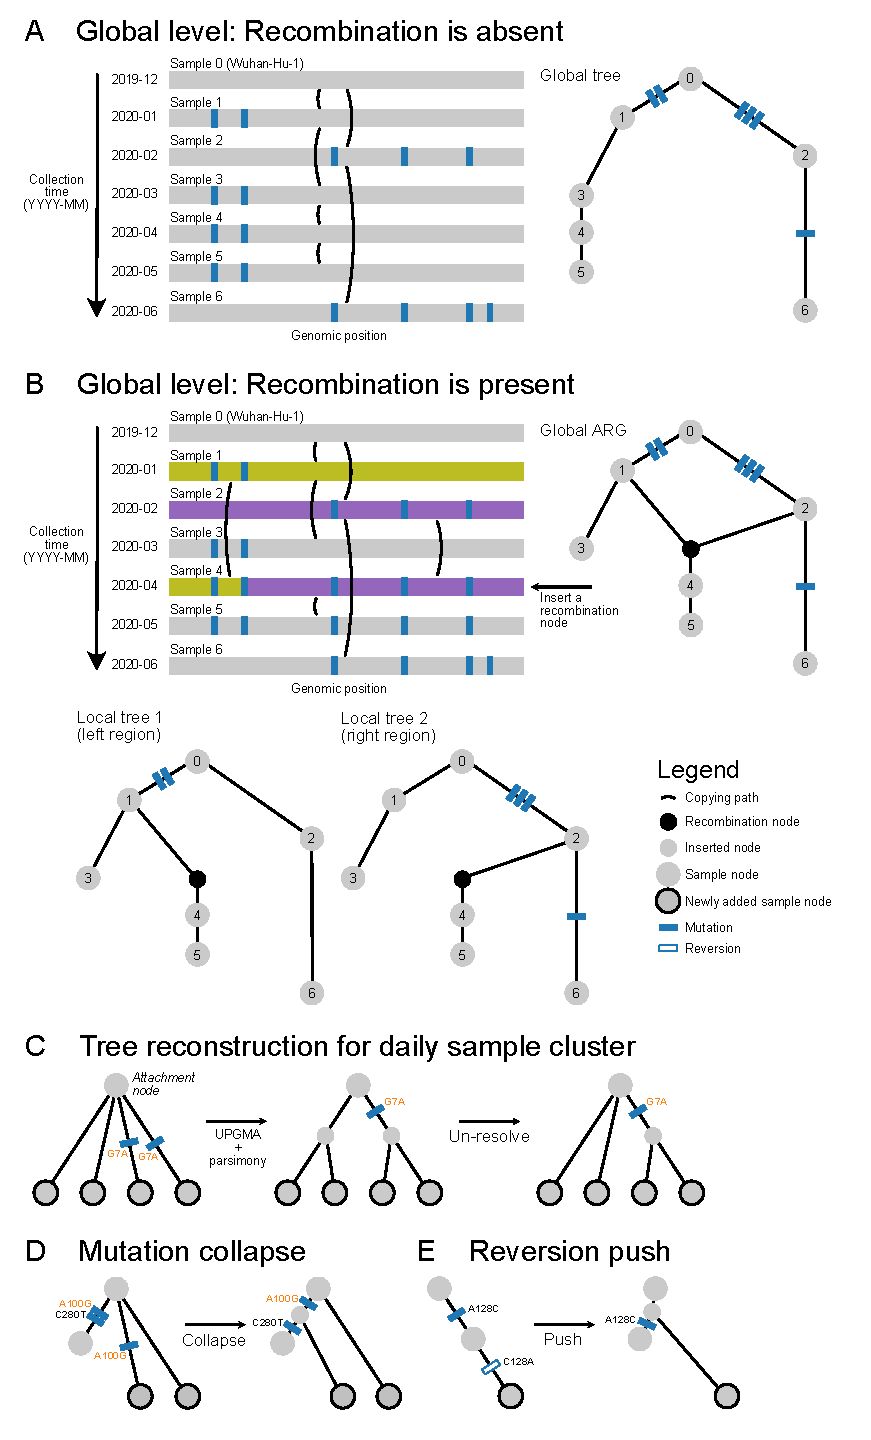
\includegraphics[width=0.7\textwidth]{figures/overview_sc2ts.pdf}
\caption{\label{fig:overview_sc2ts}
A schematic of the \texttt{sc2ts} method.
Sc2ts reconstructs the genetic relationships
among SARS-CoV-2 genomes by copying samples to all possible ancestors collected
at earlier time points (curved arrows). Each daily iteration involves three stages:
(1) attachment of new samples to the growing ARG (A, B); (2) reconstruction of
trees relating the samples under each attachment node (C); and parsimony-based
tree topology adjustments (D, E). In the absence of  recombination, sc2ts
infers an ARG that is a single tree relating the samples (A). However, in the
presence of recombination, sc2ts infers an ARG that is encoded as a sequence of
local trees relating segments of the sample genomes (B), inserting a
recombination node to represent a putative recombination event. Additionally,
mutation-collapsing nodes (D) and pushed-reversion nodes (E) are inserted to
make more parsimonious placements of mutations that should be shared or should
not be immediately reverted, respectively.}
\end{figure}


% We introduce an ARG inference method, summarised in
% Figure~\ref{fig:overview_sc2ts}.
% % Note going to rewrite this anyway, so not trying to make it flow.
% It uses (1) an efficient HMM implementation of the Li and Stephens (LS) model
% \citep{Li2003-ib} to copy SARS-CoV-2 genomes (see Sections 2.2 and 2.3); (2)
% the reported collection dates of the SARS-CoV-2 samples to determine the order
% of genome copying; and (3) several parsimony-based heuristics to locally refine
% the topology. In brief, this combined approach uses the likelihood model of LS
% to attach sample genomes to existing nodes and to detect recombinants, but
% because many of the daily tip samples harbour few, if any, mutational changes,
% we use parsimony to resolve their close relationships.

% Our HMM implementation, sc2ts, builds a reticulated graph for SARS-CoV-2 by
% taking advantage of the reported collection dates to incrementally grow the
% ARG. The inference process occurs forward in time, attaching new genomes
% aggregated by their collection date (daily batches), from the earliest to the
% last collection date. Prior to attaching sample genomes, the ARG is initialised
% such that the Wuhan-Hu-1/2019 reference genome is the root node. In the absence
% of recombination, the ARG is a single tree with no reticulation (Figure 1A);
% however, in the presence of recombination, a reticulate ARG is generated, with
% variation in tree topology across the genome (Figure 1B). Unlike standard
% phylogenetic trees in which internal nodes always represent inferred ancestors,
% internal nodes in the sc2ts ARGs represent sequences which can either be
% inferred ancestors or known samples.

% Each daily batch of genomes is first attached to the growing ARG without any
% phylogenetic resolution. In cases where the newly added sequence is inferred to
% be a recombinant, a recombination node is inserted; the ``date'' of this node
% is arbitrarily set to the average of the collection dates of the genome and the
% most recent of its parent nodes. Otherwise, the genomes are attached to the
% most closely related ancestral node (an attachment node). This creates
% polytomies that are then locally resolved among the descendants of each
% attachment node using the Unweighted Pair Group Method with Arithmetic Mean
% (UPGMA) algorithm \citep{Michener1957-tr}, with average linkage (Figure 1C).
% This hierarchical clustering algorithm produces a dendrogram relating a set of
% sequences, which is treated as an ultrametric binary tree here. Subsequently,
% mutations are placed onto the daily tree by maximum parsimony. An issue with
% the UPGMA algorithm is that it may create internal nodes supported by no
% informative site (i.e., having no mutation immediately ancestral to them). In
% an adjustment step, such unsupported internal nodes are removed to
% ``un-resolve'' the daily tree; the remaining internal nodes, which are
% supported by at least one shared mutation, are retained. The ``dates'' of the
% non-sample internal nodes are set to the same date as the samples in the daily
% batch. The resulting daily tree is grafted onto the attachment node in the
% global ARG.

% During ARG inference, two types of non-sample nodes are inserted to improve
% parsimonious placement of mutations: mutation-coalescing nodes and
% pushed-reversion nodes. We call these operations tree adjustments. A
% mutation-collapsing node is inserted when a shared mutation between sibling
% nodes is found (Figure 1D). An attempt to create mutation-collapsing nodes is
% made after grafting a new daily tree onto the global ARG. If shared mutations
% exist between two or more sibling nodes, then a parsimonious explanation is to
% create a new node that is the parent of those siblings, on which these
% mutations occurred. A pushed-reversion node is inserted when an immediate
% reversion occurs (Figure 1E), i.e. a mutation that reverts another mutation on
% its parent node. Instead of retaining both the mutation and immediate
% reversion, only the mutation is kept after a pushed-reversion node is inserted,
% thereby reducing the number of mutations on the branches. Note that these
% non-sample nodes are used as reconstructed genomes during HMM copying.

% Furthermore, during inference, the ARG is automatically encoded, stored, and
% updated as a tree sequence using tskit \citep{Kelleher2018-xc}.

\subsection{Ancestral Recombination Graphs}
\label{sec:args}
The term ``Ancestral Recombination Graph'' was introduced by
Griffiths and colleagues~\citep{Griffiths1991-two,Griffiths1998-ancestral}
and originally defined as an alternative formulation of the coalescent
with recombination stochastic process~\citep{Hudson1983-properties}.
Subsequently, the term ARG came to be used in a more general way to
describe not just realisations of this model, but to any
recombinant genetic ancestry~\citep{Minichiello2006-mapping,Zhang2023-lf}.
While there is some subtlety in the details~\citep{Wong2023-efficient},
we can think of an ARG as being any graph that encodes the
reticulate genetic ancestry of a sample of colinear sequences under
the influence of recombination.
This definition encompasses various types of graphs often
described using the broader term of phylogenetic networks.

The ``succinct tree sequence'' is an ARG data structure
that is both general (in terms of the types of ancestry that can
be described) and computationally efficient~\citep{Wong2023-efficient}.
Originally developed to facilitate large-scale coalescent
simulations~\citep{Kelleher2016-wk}, the methods have been
extended and applied to forwards-time
simulations~\citep{Kelleher2018-xc,Haller2018-tree},
calculation of population genetics statistics~\citep{Ralph2020-efficiently}
and ARG inference~\citep{Kelleher2019-ba,Wohns2022-th}.
The succinct tree sequence is based on a simple tabular representation,
which defines a set of nodes, edges, sites and mutations. A \emph{node}
represents a particular genome, which may be an observed sample
or an inferred genetic ancestor. The genetic inheritance between
a pair of nodes along a segment of genome is defined by
the \emph{edge} $(\ell, r, p, c)$, which states that
child node $c$ inherited its genome from parent node $p$
from left coordinate $\ell$ to right coordinate $r$. A \emph{site}
defines the genomic position at which some variation occurs,
and a \emph{mutation} defines the site, node and derived state
that generates variation.
% JK: Note sure this clarifies much at the representational level?
% (note that this requires that the sequences can be aligned and phased).

Given these tables, we can then efficiently construct the local
genealogical trees along the genome (arising from recombination),
and also perform a range of calculations efficiently by
reasoning about the differences between these local
trees~\citep{Kelleher2016-wk,Ralph2020-efficiently}. These
algorithms have led to performance increases of several orders
of magnitude over the state-of-the-art in a range of
applications~\citep{Kelleher2016-wk,Kelleher2018-xc,Kelleher2019-ba,
Ralph2020-efficiently,Baumdicker2022-ep}.
The succinct tree sequence encoding
is also very concise, allowing, for example, for millions of
complete human genomes to potentially be stored in a few gigabytes of
space~\citep{Kelleher2019-ba}.

The \texttt{tskit} library~\citep{Tskit2023-tskit} is a liberally
licensed open source toolkit that provides a comprehensive suite
of tools for working with ARGs. Based on core functionality written
in C, it provides interfaces in C, Python and Rust. The Python interface
is based on NumPy~\citep{Harris2020-array}, and provides a convenient
platform for interactive analysis of large-scale data using, for
example, Jupyter notebooks~\citep{Kluyver2016-jupyter} and taking
advantage of the analysis tools in the burgeoning PyData ecosystem.
(It is possible to access the toolkit from R via the \texttt{reticulate}
package, and the \texttt{slendr} library~\citep{Petr2022-slendr}
also provides some native R support. A full R interface would be a
valuable addition to the ecosystem.)
Tskit is mature software, widely used in population genetics, and
has been incorporated into several downstream
applications~\citep[e.g.][]{Haller2019-slim,Speidel2019-yh,
Terasaki2021-geonomics,
Fan2022-genealogical,Korfmann2022-weak,
Mahmoudi2022-bayesian,Petr2022-slendr,Rasmussen2022-espalier,
Zhang2023-lf}.
It is important to note that
this ecosystem for storing and manipulating ARGs can
generally be used to efficiently record and analyse SARS-CoV-2 genealogies reconstructed
using other methods, not only the \texttt{sc2ts} approach that we describe here.
Note also that there is no requirement that recombination be present,
and the methods are also very efficient when working with a single tree.

\subsection{The Li and Stephens model}
\label{sec:ls}
The Li and Stephens (LS) model \citep{Li2003-ib} is an approximation of the
coalescent with recombination~\citep{Hudson1983-properties}, which captures
many of the important features of the joint processes of mutation and
recombination. It is a Hidden Markov Model (HMM) in which a focal genome
is modelled as a
sequence of nucleotides that are probabilistically emitted as
an imperfect mosaic of a set of reference genomes
(Figure~\ref{fig:ls_diagram}).
The LS model is used in a wide variety
of applications in genomics, including modern approaches to
statistical genotype phasing and imputation
\citep{Delaneau2019-wl,Browning2021-cg,Browning2018-nk,Rubinacci2020-pa},
and estimation of parameters such as
recombination rates \citep[e.g.][]{Hinch2011-tz},
and selection within and across hosts in viral
sequence data \citep[e.g.][]{Palmer2019-wa}.
See~\cite{Mcvean2019-linkage} for further review and discussion
of the LS model.

\begin{figure} \centering
\includegraphics[width=0.5\textwidth]{figures/ls_diagram_covid.pdf}
\caption{\label{fig:ls_diagram} A schematic of the Li and Stephens (LS)
model, in which a query sequence (bottom) is described as an
imperfect mosaic of the sequences in a reference panel.
Black crosses along the focal sequence show sequencing
errors or mutations.
In the standard formulation, at site $\ell$, the recombination probability is $r_\ell$,
the mutation probability is $\mu_\ell$ and $n$
denotes the size of the reference panel.
The Viterbi algorithm can be used to find a
``copying path'' through the reference panel for a given query sequence that
maximises the likelihood under these parameters. Unseen states in the reference panel are shown as coloured lines enclosed by
the grey box. The black arrow describes the true path through the data which leads to the emitted
focal sequence below. Examples of transition and
emission probabilities along this trajectory are shown by the red and blue
arrows, respectively.
}
\end{figure}

% The LS HMM is governed by the transition and
% emission matrices, $Q$ and $E$, respectively.
%
% These two
% processes, transition and emission (which encode recombination and mutation,
% respectively), define the generative process of the HMM, by which an imperfect
% mosaic is emitted from a reference panel.
 % of samples and nodes from the ARG
% inserted at earlier collection dates (shown in the lower panel). Here, the
%
% Note that in practice, we do not know the pattern of
% colours along the focal sequence and must infer it using the Viterbi algorithm.

The generative process of the LS model is summarised in
Figure~\ref{fig:ls_diagram}. Here, a transition matrix, $Q$, governs the
process of switching (recombining) between members of the reference panel (the
hidden states). An emission matrix, $E$, allows for differences between the
focal sequence and the hidden state from which it is copied (due to mutation as
well as sequencing error).
Both $E$ and $Q$ may be a function of the reference panel members,
but transitions are generally assumed to be independent of the
hidden states (Figure~\ref{fig:ls_diagram}, pink panel).
This assumption dramatically increases performance as the state space drops to two states (i.e., switching or not switching).
Emissions may also be a function of the nucleotide states, but in our
case, we assume that all observed alleles (in both the reference panel and
focal sequence, $a_\ell$) at the site under consideration are equally likely and
occur with mutation probability $\mu_\ell/(a_\ell-1)$
 (Figure~\ref{fig:ls_diagram}, blue panel).
We use the Viterbi algorithm~\citep{Viterbi1967-ol}
to find the most likely copying path, given a set of reference sequences, $Q$, and $E$.
Throughout, we refer to the probabilities of mismatching to a
member of the reference panel at site $\ell$ as $\mu_\ell$,
and the probability of recombining between two members of the reference panel between site $\ell-1$ and site $\ell$ as $r_\ell$. For convenience, $\mu_\ell$ is commonly referred to as the `mutation probability', but we note that this probability of
mismatch also encompasses various other error modes which result in a mismatch
(such as sequencing and alignment errors). Note also that it is these probabilities,
not the rates of mutation and recombination, that are required to fully define the HMM.
That said, we can approximately relate these probabilities to the coalescent with recombination process which LS is approximating. In the case of recombination,
suppose that there is some constant underlying recombination rate, $\rho$.
Assuming that recombination events occur as a Poisson process,
then the probability of recombining between adjacent sites is
\begin{align*}
    r_\ell = 1 - \exp\left(-\frac{\rho\left(m_{i-1} - m_{i}\right)}{n}\right),
\end{align*}
where $m_j$ is the nucleotide position of variant $j$.
Similarly, we may consider the probability of mutation to represent to the
probability of mutation along the branch joining the focal sequence to a coalescent
tree containing a reference panel with $n$ members, assuming a Poisson process
along the branch. The expected length of this branch is $4/n$, and so the mismatch
probability represents the probability of observing a mutation or error mode,
along this branch. We can then approximate the probability of observing a mismatch as:
\begin{align*}
    \mu_\ell \approx 1 - \exp{\left(-\frac{4\nu}{n}\right)}
\end{align*}
where $\nu$ is the mutation rate per $\mbox{ploidy} \times N_e$ generations.

The probabilities of these competing process of mismatch and recombination are
usually controlled by the site-specific parameters $\mu_\ell$ and $r_\ell$,
respectively. For this work we used a slightly different formulation, which
uses one parameter, the mismatch ratio (MMR), to control the relative
importance of mutation and recombination in the HMM. Specifically, an MMR value
of $k$ will prefer $k$ mismatches (mutations) to a single recombination which
results in copying from a template with no mismatches. To map between
recombination probability and mutation probability for a particular mismatch
ratio, we simply consider the two paths which we wish to be equally likely, and
rearrange for the mutation or recombination probability. Consider the simple
case when we assume $\mu_l=\mu$ and $r_l=r$. Without loss of generality,
consider a region of length $m$. Up until this region, two paths are equally
likely, so we can re-scale by the likelihood of observing the focal sequence up
to the site before the region starts, $c$. For an MMR of $k$, we only need to
consider two of the $n$ members of the reference panel.

One, $\mathcal{P}_1$,
for which there are no mismatches, but we need to recombine in, and a second,
$\mathcal{P}_2$, for which there are $k$ (randomly chosen) mismatches in the
region.
Now, follow the probability of tracking along each of those paths:
\begin{align*}
\mathbb{P}[\mathcal{P}_1] &= \frac{cr}{n}
\left(\left(1-r\right)+\frac{r}{n}\right)^m\left(1-\mu\right)^m
&\text{recombine to a template with no mismatches,}\\
\mathbb{P}[\mathcal{P}_2] &= c
\left(\left(1-r\right) +
\frac{r}{n}\right)\left(\left(1-r\right)+\frac{r}{n}\right)^m
\left(1-\mu\right)^{m-k}\mu^k &\text{stay in a template with $k$ mismatches,}
\end{align*}
% where $r$ is the recombination probability between adjacent
% variants, $\mu$ is the mismatch probability between a target sequence at a
% variant and a particular member of the reference panel,
where $c$ is the
likelihood of the path up to this point, which are assumed to be
equal by construction.
We then
set these path probabilities to be equal, and rearrange to obtain:
\begin{align*} r = \frac{n\mu^k}{\left(1-\mu\right)^k + \left(n-1\right)\mu^k},
\quad\quad \mu = \frac{1}{\sqrt[k]{\frac{n}{r} - (n-1)} + 1}. \end{align*}
Thus, for lower MMR values ($k$ here),
recombinations are favoured over mutations
than a single ancestral genome. We use an MMR value of $k=3$ in this work,
as it provided results that tallied well with empirical observations.
Exploring different mismatch ratios, and more sophisticated parameterisations
of the HMM are important avenues for future work.

A varying degree of missingness is present in the genetic data, that is, for a
given sample, a subset of nucleotides coded as `unknown' at a set of positions.
As a result, we had to consider missingness in our implementation of the LS
Viterbi algorithm. One approach would be to `impute' all missing data
beforehand using external software to hard-call or define a distribution over
the possible missing nucleotides, and use that in the determination of path
probabilities. Another is to not attempt to estimate the true nucleotide, but
rather to consider such sites as uninformative to the path probability, and
impute missing data within that path on the fly, placing them within the
the emission probability transition from unknown to
the emission probability from unknown to
to any other state as 1.
% $\mbox{N} \rightarrow \star$ as 1.

In \texttt{sc2ts}, we use the efficient ARG-based implementation of the
LS Viterbi algorithm from \texttt{tsinfer} \citep{Kelleher2019-ba} to find
the most likely copying path for each sample sequence
among all sequences (sampled and inferred) in the current ARG.
In the majority of cases, with non-recombinant sample sequences,
the most likely solution is to copy from one
of the nodes in the ARG that minimises the number of mutations required
to insert the query sequence. Importantly, because the reference panel here consists of
\emph{every} node in the ARG, we can match to both older sample
sequences or internal nodes representing an inferred ancestral sequence
(see subsequent subsections for details about how these are added).
Thus, when no recombination is present, the LS Viterbi algorithm is
implementing a version of parsimony, in which we are guaranteed to
find a sequence that minimises the number of additional mutations required
to incorporate a newly-added sample into the ARG.
Recombination is then inferred when the most likely solution to the LS
HMM is to copy from more than one ARG node along the genome, for a
given sample sequence.

The Viterbi algorithm enables us to find a path through
the reference panel from among the $n^m$ paths that is provably at the
optimum, under the LS model.
We can solve this massive optimisation problem exactly because the ARG-based
implementation of the LS HMM used in \texttt{tsinfer} scales approximately
logarithmically with reference panel size (as opposed to linearly,
for standard matrix-based approaches).
This efficient HMM algorithm is the main reason for \texttt{tsinfer}'s
scalability, and here allows us to find closely matching
sequences and recombination paths among millions of SARS-CoV-2
genomes exactly under a well-defined statistical model.

It is important to note that the Viterbi algorithm only returns \emph{one of}
the copying paths that maximise the likelihood under the given mutation and
recombination parameters. There may be many such paths, from which we choose
one arbitrarily. Also, the present choice of using a single mismatch-ratio
parameter to control the likelihood of recombination vs mutation may lead to
relatively flat likelihood spaces where many different paths have equal
likelihood.
There are many possibilities in using established HMM methodology
to reason about and explore the space of possible matches, which may be a
fruitful avenue for future work.
% Could talk about running the HMM in reverse here, but is there much
% point? It's confusing the main point which is that there lots of
% ways in which this could be done properly.
Examples include stochastic traceback~\citep[e.g.,][]{rasmussen2014genome}
through the collection of paths at the global optimum to glean further
information about our the likelihood surface, and determine whether there are
downstream implications for our conclusions. Here, we have considered the
Viterbi algorithm to make statements about the most likely paths through the
data. The machinery used here can be modified to run the forwards and backwards
algorithms which determine the probability of observing a focal sequence,
integrating over all possible paths through the data, under the LS
model~\citep{Palmer2023-efficient}.
This presents an opportunity to estimate parameters of interest
under the LS model at pandemic scale.

\subsection{Tree inference from HMM daily sample clusters}
\label{sec:sample-cluster-tree-inference}
For a given daily batch of sample sequences that are to be attached to the
ARG, the LS HMM provides the most likely copying path and required mutations
for each of those sequences. We could directly attach these samples to
the ARG according to the copying paths and sets of mutations, but
such an approach would be highly unparsimonious because there are
often many samples that share the same copying path, with
complex patterns of shared mutations among those clusters of samples.
In this section we discuss the strategy used to infer likely tree
topologies within these clusters of samples sharing the same copying path.
In the majority of cases the copying path will consist of a single
node (i.e., no recombination), and so for simplicity we will assume in the
following discussion that all of the samples in a HMM-defined cluster
attach to a single node. The special treatment afforded to
newly-detected putative recombinants are discussed
in Section~\ref{sec:treatment_recombinants}.

With tens of thousands of samples being added to the ARG per day,
there are often clusters of hundreds of sequences attaching to the same node.
While some of these samples will require no extra mutations
(because they are identical to the attachment node), in general there
will be complex patterns of shared mutations among the samples
reflecting their evolutionary relationships. A natural way to infer
these within-cluster evolutionary relationships is to use standard
tree-building algorithms.
We can infer a likely tree relating the
samples in a cluster independently of the other samples in a
daily batch, and then attach the tree (and mutations)
to the ARG at the node identified by the HMM.

We currently use the UPGMA algorithm~\citep{Michener1957-tr}
as implemented in SciPy~\citep{Pauli2020-scipy} to build trees from sample
clusters, and map mutations back to this topology using maximum parsimony.
This approach was chosen mainly for simplicity and because of the
speed and reliability of the implementation.
An issue with the UPGMA algorithm is that it generates a strictly
binary tree, creating internal nodes
supported by no informative site (i.e., having no mutation immediately
ancestral to them). We avoid such false precision by post-processing
to remove unsupported internal nodes, representing the relationship
between $k$ identical descendants of a node as a polytomy of size $k$.

There are well-known issues with using such a simple algorithm for inferring
evolutionary relationships~\citep{Felsenstein2004-inferring}.
Table~\ref{tab:args} show that
this within-cluster tree building has a significant influence on the
overall ARG topology (Wide ARG: 7.05\% of nodes and parent of
32.27\% of edges; Long ARG: 6.61\% and 19.97\%, respectively),
and therefore applying more sophisticated
tree building methods which keep track of the required mutations
(rather then inferring post-hoc by parsimony), is a likely avenue
for improvements in overall inference quality.

\subsection{Parsimony-increasing heuristics}
\label{sec:parsimony-heuristics}
Attaching trees built from the clusters of samples that copy from
a particular node (or path of nodes for recombinants,
see Section~\ref{sec:treatment_recombinants}) under the
HMM is an inherently greedy strategy,
and can produce inferences that are clearly unparsimonious.
The final step in adding a daily batch of samples to the ARG
is therefore to perform some local updates that target specific
types of parsimony violation in the just-updated regions of the
ARG. There are currently two parsimony-increasing operations
applied, which we refer to as ``mutation collapsing'' and ``reversion
pushing'' (Figure~\ref{fig:overview_sc2ts}D, E).

Mutation collapsing inspects the siblings of a newly attached node
to check if any of them share (a subset of) the mutations that
it carries. If so, we increase the overall parsimony of the inference
by creating a new node representing the ancestor that carried
those shared mutations, and make that new node the parent of the
siblings carrying those shared mutations. The patterns of
shared mutations between siblings can be complex, and the current
implementation uses a simple greedy strategy for choosing
the particular mutations to collapse.
Table~\ref{tab:args} shows that
while these nodes constitute a small fraction of the
overall total (Wide ARG: 2.77\%, Long ARG: 4.82\%),
they are parental to a much larger fraction of the
edges (Wide ARG: 12.77\%, Long ARG: 20.47\%).

The reversion push operation inspects a newly added node to see
if any of its mutations are ``immediate reversions''; that is,
are reversions of a mutation that occured on the new node's
immediate parent. We increase the overall parsimony of the
inference by ``pushing in'' a new node which descends from the
original parent which carries all its mutations except those
causing the reversions on the newly added node.
Table~\ref{tab:args} shows that
these nodes constitute a similar fraction of the
overall numbers of nodes (Wide ARG: 2.79\%, Long ARG: 4.39\%)
and edges (Wide ARG: 12.66\%, Long ARG: 18.46\%)
as mutation collapsing.

Together these operations substantially increase the overall parsimony
of the inferred ARGs, most noticably in terms of the number of
reversion mutations inferred. These nodes are also being chosen by the
LS HMM as likely choices of parent (as indicated by the node and edge
counts quoted above), also demostrating that the hueristics are successfully
capturing features of real sequences.
However, they are both simple
greedy operations, just examining the local parts of the
ARG topology affected by newly added samples. Since the inferred
ARGs still contain a large number of reversion mutations which
are likely to be mostly artefactual, it is clear that there
is room for improvement, and that further parsimony-increasing
heuristics would likely be of benefit.

\subsection{Treatment of recombinants}
\label{sec:treatment_recombinants}
A sample sequence is designated as a recombinant if the most likely
path inferred by the LS HMM for that sample contains at least
one switch between parents. Recombinant sequences are mostly treated
identically to non-recombinants, as we simply need to reason about
a path of parent nodes along genome intervals rather than a
single parent over the whole genome, which is naturally handled by
the succinct tree sequence data structure and \texttt{tskit} library
(Section~\ref{sec:args}). To facilitate
analysis and to help understand the robustness of recombinants
we perform some additional steps in \texttt{sc2ts}.

The LS HMM may infer identical paths and patterns of mutations
for multiple samples in a daily batch, and so we
create a ``recombination`` node (marked with a specific ``flags'' value)
for each distinct recombinant. (This node is not strictly necessary
but makes it convenient to find recombinants for subsequent analysis.)
Variation within a cluster
of recombinant sequences is handled in the same way as non-recombinants
(see Section~\ref{sec:sample-cluster-tree-inference} above for details).
When the Viterbi algorithm implementation used by the LS HMM infers
recombinant ancestry for a given genome, the point at which inheritance
switches from one parent node to another is the last possible
position. The left-most extent of the breakpoint interval is derived
by sequence comparison between the parents, as described in
Section~\ref{sec:breakpoint_intervals}.

% Thus, the breakpoints used in the ARG represent the rightmost end of the
% interval, within which the recombination event could have occurred. To obtain
% the leftmost end of this interval, we rerun the HMM using mirrored coordinates
% (i.e., from the 3’ end to the 5’ end) and store the information as
% metadata on the recombination node.
% These left- and rightmost positions
% are the recombination intervals reported throughout.
% Ultimately all the recombination intervals mean is that the parent sequences
% are identical within that interval, and there is therefore no information
% about where the recombination occurred. There are many different processes
% that can contribute to the size of these intervals, and therefore
% understanding how these processes interact to produce wider or narrower
% intervals is an important avenue for future work.

The LS HMM machinery, and the interpretation of inferred recombinant paths and
breakpoint intervals is a central part of \texttt{sc2ts}, and there are many
ways to extend and improve. For example, the current parameterisation of using
a single ``mismatch ratio'' is very simplistic (Section~\ref{sec:ls}), and likely
results in a flat likelihood space where many recombinant paths have equal
probability of being chosen.
More sophisticated parameterisations where we
condition on known per-site mutation rates (and perhaps per-base subsitution
rates) may lead to better results, although perhaps at the cost of some
reduction in interpretability. Post-processing the match results to produce
more parsimonious breakpoints may also be a worthwhile avenue for development.
In particular, we may choose to insert breakpoints for the ARG that are chosen
from within the possible interval, rather than the current approach of taking
the rightmost value. Cases where we have more than two parents may either be
the ``stacking'' of multiple recombination events, or instances where
the HMM has chosen to switch to a third sequence rather than back to
the original parent (where this is equally parsimonious). Many putative
recombination events, however, will represent poor quality data, where
a recombinant copying path happens to be a more likely explanation
of a highly divergent sequence.
A thorough analysis of the behaviour of the LS model in the context
of a pandemic-scale ARG may lead to significant improvements in our
ability identify recombinants and to filter poor quality data.

\subsection{Node dating}
\label{sec:node_dating}
The approaches to assigning a date to nodes in \texttt{sc2ts} is currently
ad-hoc, and the inferred timing of events from the ARGs reported
here should be treated with caution (e.g., Figure~\ref{fig:recomb_mrcas}).
Sample nodes (those corresponding to observed sample sequences) are the
most accurately dated, as we use the reported collection date for
these nodes. These are not entirely accurate, but our data filtering
criteria should remove the most egregious errors (see
Section~\ref{sec:filtering_time_travellers}). Other nodes in the ARG
are dated by splitting the time between the attached samples
and the chosen parent nodes equally (in the case of
trees inferred from daily sample clusters,
Section~\ref{sec:sample-cluster-tree-inference}) or by adding arbitrary
small values when creating new nodes using parsimony rules
(Section~\ref{sec:parsimony-heuristics}). Since the ARGs here are
very treelike, with recombination nodes consituting a tiny fraction
of the overall topology (Table~\ref{tab:args}), existing methods
\cite[e.g.,][]{to2016fast} could likely be adapted to accurately
date the vast majority of the nodes.

\subsection{Data preprocessing}
\label{sec:data_preprocessing}
The findings of this study are
based on sequences and metadata available on GISAID (\url{https://gisaid.org/})
up to 2022-08-22 and accessible at
% Do we need to upload a separate Table or is this DOI sufficient?
\url{https://doi.org/10.55876/gis8.230329cd}.
We removed sequences
if they had ambiguous collection dates, were collected before 2020-01-01
or were isolated from a non-human host.
We aligned sequences to the Wuhan-Hu-1/2019 reference sequence
(GenBank: MN908947.3) using Nextclade v2.3.0~\citep{Aksamentov2021-hj} (dataset tag
2022-07-26T12:00:00Z). We also excluded sequences if they had a
``bad'' quality control status
in any of the four Nextclade columns (``qc.missingData.status'',
``qc.mixedSites.status'', ``qc.frameShifts.status'' and `qc.stopCodons.status'').

We encode ambiguous nucleotide letters (i.e.,
not A, C, G, T, or a gap) in the pairwise genome alignments as missing data
(N). Problematic bases in the alignments, which had two or more Ns or
gaps within a distance of seven bases, are masked as missing data following
the approach used in the ``faToVCF'' tool used by
UShER~\citep{Turakhia2021-ur}.
Sites that are masked by this process are
treated as missing data by the LS HMM (Section~\ref{sec:ls}).
In addition, we exclude 481 problematic sites flagged as prone to
sequencing errors or as highly homoplasic
(\url{https://github.com/W-L/ProblematicSites_SARS-CoV2/},
accessed 2022-09-22) entirely.

Although the masking strategy used currently is simple and robust,
there are significant disadvantages, excluding, for example, any
deletions of length greater than one base. Exploring more sophisticated
masking strategies is an important route for future improvements.

\subsection{Filtering ``time travellers''}
\label{sec:filtering_time_travellers}
A major source of error in early versions of \texttt{sc2ts} was
the existence of ``time traveller'' sequences: those with erroneously
early collection dates.
For example, an Alpha sample purportedly collected in 2020 from the United States,
before Alpha appeared in the United Kingdom (USA/MN-Mayo-1563/2020),
produced significant topological distortions in
inferred ARGs.
Hence, to exclude such potential ``time travellers'' we employ two filters.

The first filter is a simple threshold on
the time delay between the collection date and submission date.
After some preliminary analysis we settled on a maximum submission delay
of 30 days when building the ARGs described here.
The second filter is to remove any sequence with a collection date that
pre-dates the
time to the most recent common ancestor (tMRCA) of its corresponding clade.
We obtained the tMRCA for each clade from a Nextstrain GISAID reference tree
(downloaded on 2022-08-22), and we used the lower bound of the 95\%
confidence interval of each clade as the minimum date cut-off.
This excludes a further 618 samples not covered by the maximum submission
delay filter.

As the results of \texttt{sc2ts} are sensitive to the existence of
time-travellers, an important aspect of future work is to find better ways
to identify them. One possibility is to use the LS HMM itself to flag
overly divergent sequences, and to exclude them from attachment to the ARG.
We might also estimate collection dates by adding these potential time travellers
back to the ARG, allowing an automated assessment of collection date discrepancies.

\subsection{Imputation of Pango lineage for non-sample nodes}

\begin{figure} \centering
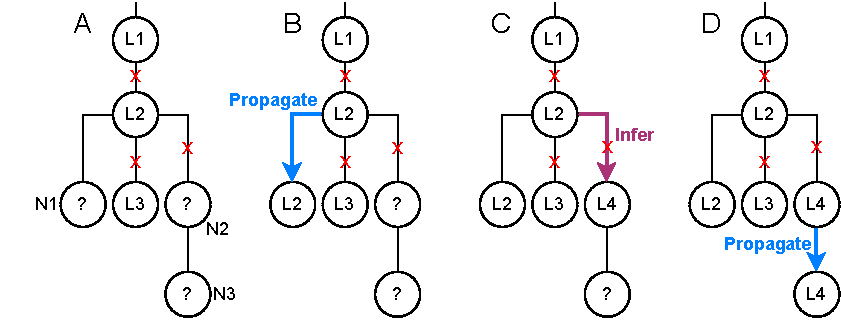
\includegraphics[width=.7\textwidth]{figures/imputation.pdf}
\caption{\label{fig:imputation}A schematic of the iterative procedure to impute
Pango lineage for inserted, non-sample nodes. Here, three nodes (question
marks) have unknown Pango lineage (A). The lineage for node N1 can be directly
copied from its parent (L2). The lineage for node N2 must be inferred from
that of the parent (L2) plus the lineage-defining mutation (red X)
on the connecting edge. The lineage for node N3 can then be copied from
that of node N2.}
\end{figure}
While the Pango lineages of sample nodes are imported directly from
GISAID metadata, the lineage status of internal nodes inserted into
the \texttt{sc2ts} ARG must be imputed. We do this using
the list of lineage-defining mutations (based on 90\% consensus
of the sequences analysed) from the
COVID-CG website \citep[][\url{https://covidcg.org/};
accessed on 2022-11-04]{Chen2021-zc}.

For a given non-sample node $u$, if the Pango lineage of its parent or
one of its children is already known, and there are no lineage-defining mutations
on the connecting edge, then $u$ copies this Pango lineage exactly.
Otherwise, the lineage for $u$ is inferred by
matching its full set of mutations against the COVID-CG list.
We apply these two steps to the internal nodes of the ARG iteratively,
as illustrated in Figure~\ref{fig:imputation}, until all internal nodes
are assigned a lineage (where possible---note that sometimes a lineage cannot
be assigned to the children of a recombination node).

This method is fast, as the lineages for most of the internal nodes can be
imputed by copying from the surrounding nodes
(Wide ARG: 80\% of nodes,
Long ARG: 66\%),
and significantly more efficient than extracting
the haplotypes for each internal node and using existing Pangolin assignment tools
\citep{OToole2021-assignment}. The
accuracy depends on the quality of the list of lineage-defining mutations,
as well as the source of lineage designation for the sample nodes: we obtain
slightly different results when using those recorded on GISAID (which uses
pangoLEARN), and those assigned by Nextclade. To gauge the accuracy of
imputation, we have used our method to re-impute the lineage designations of each
sample node using the surrounding information; this results in
99\% of nodes being assigned the same lineage as per the source metadata in the
Wide ARG, and 98\% in the Long ARG.

\section{Acknowledgements}
We gratefully acknowledge all data contributors, i.e., the Authors and their
Originating laboratories responsible for obtaining the specimens, and their
Submitting laboratories for generating the genetic sequence and metadata and
sharing via the GISAID Initiative, on which this research is based.
% Not using these now:
% Also, we
% thank Dr. Morag Graham (the National Microbiology Laboratory, Winnipeg, Canada)
% for kindly providing the genomic coordinates of the breakpoint sequence motifs.
SHZ is supported by the Janssen-Oxford Translational Genomics Fellowship. JK,
YW, and BJ are supported by the Robertson Foundation.

\section{Data Availability}
The source code for \texttt{sc2ts} is
available on GitHub
\url{https://github.com/jeromekelleher/sc2ts/}.
The Jupyter notebooks and code used to produce the results described here are also
available on GitHub \url{https://github.com/jeromekelleher/sc2ts-paper/}.

% TODO what's the right way to say this?
The inferred ARGs described here are available on request to those with
the appropriate GISAID data access.

\bibliographystyle{plainnat}
\bibliography{paper}

\clearpage
\renewcommand\thefigure{S\arabic{figure}}
\setcounter{figure}{0}
\renewcommand\thetable{S\arabic{table}}
\setcounter{table}{0}
\section*{Supplementary}

\begin{figure}[h] \centering
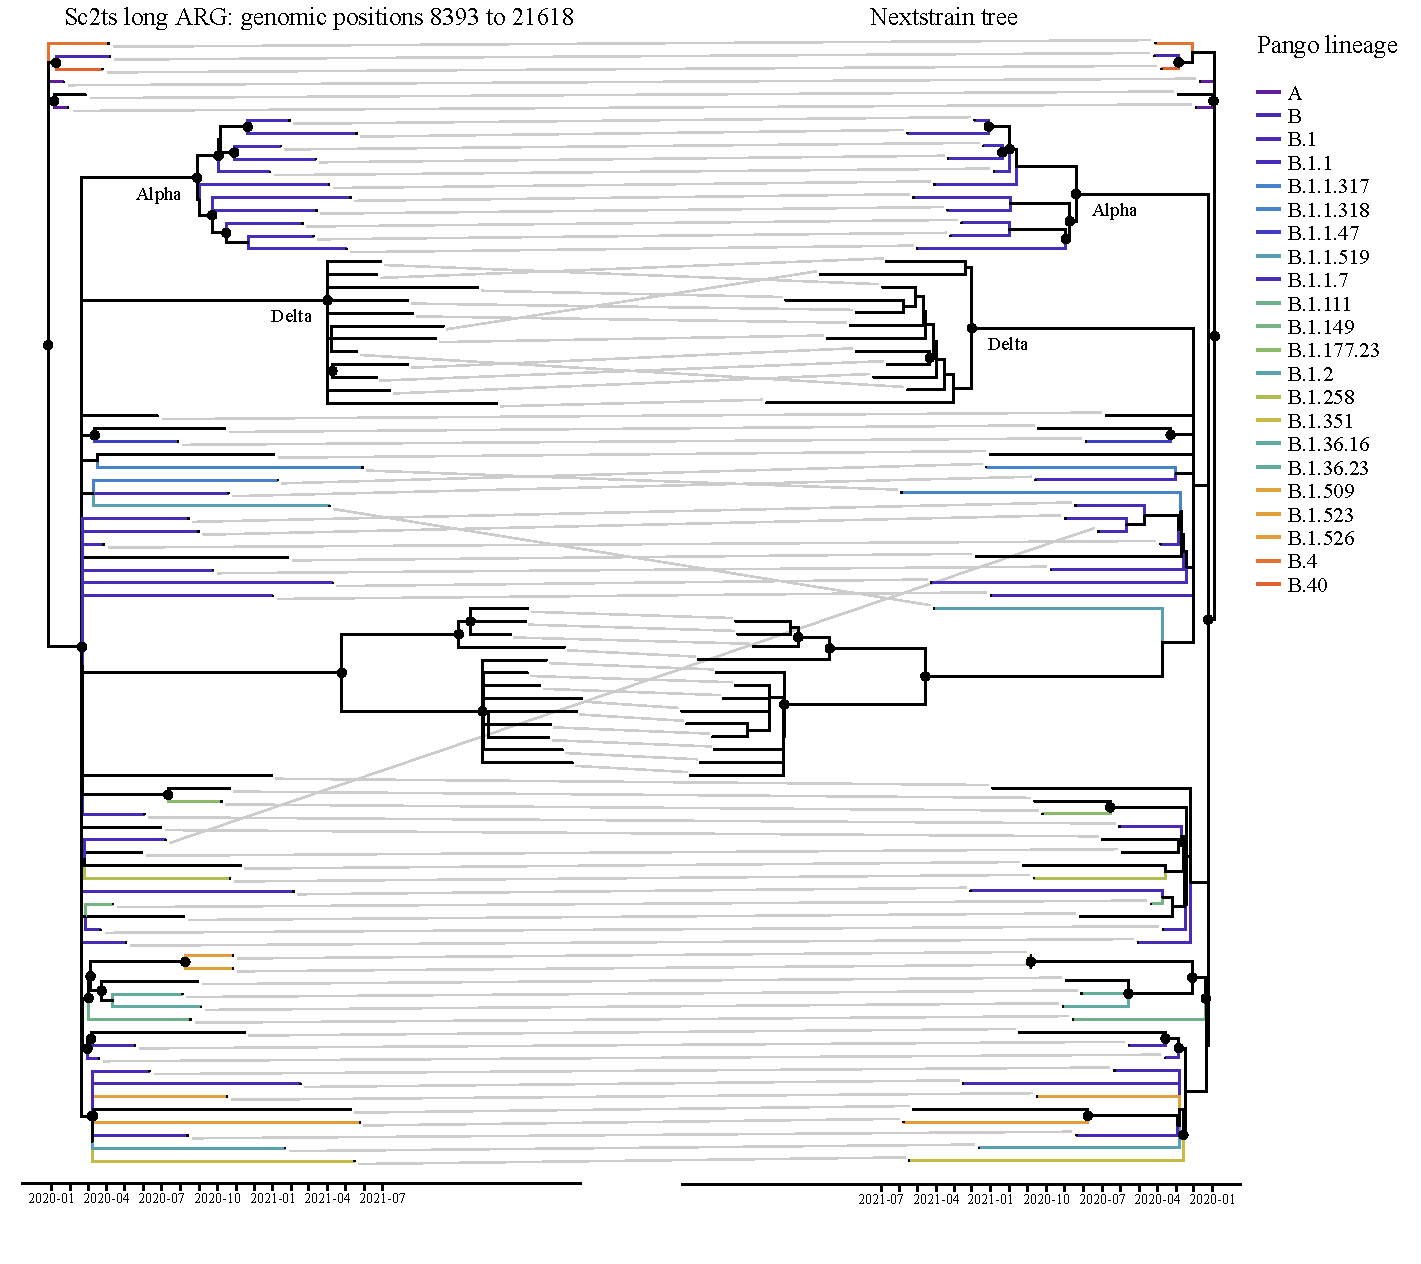
\includegraphics[width=\textwidth]{figures/supp_cophylogeny_long.pdf}
\caption{\label{fig:cophylogeny_long}Tanglegram equivalent to that in Figure~\ref{fig:cophylogeny},
but for the Long ARG (i.e. subsampled to mid-2022).}
\end{figure}

% FIXME there's too much vspace between the rows here. Probably best to redo
% the formatting.
\begin{table} \centering
\begin{tabular}{l|c|c|c|c|c} \hline
\multicolumn{1}{c}{} & \multicolumn{3}{c}{\textbf{Jackson et al. (2021)}} &
\multicolumn{2}{c}{\textbf{sc2ts (Wide ARG)}} \\ \hline
\textbf{Sample} &
\textbf{Group} & \textbf{Parents} & \thead{Breakpoint \\
interval(s)} &
\textbf{Parents} & \thead{Breakpoint \\ interval(s)} \\
\hline ALDP-11CF93B & A
    & \thead{B.1.177 \\ Alpha} & 21,255–21,613 & \thead{B.1.177.18 \\ Alpha} &
21,256–22,228 \\
    ALDP-125C4D7 & A & \thead{B.1.177 \\ Alpha} & 21,255–21,613 &
    \thead{B.1.177.18 \\ Alpha} & 21,256–22,228 \\
ALDP-130BB95 & A & \thead{B.1.177 \\ Alpha} & 21,255–21,613 &
    \thead{B.1.177.18 \\ Alpha} & 21,256–22,228 \\
LIVE-DFCFFE & A & \thead{B.1.177 \\ Alpha} & 18,998–20,294 &
    \thead{B.1.177.18 \\ Alpha} & 21,256–22,228 \\
QEUH-CCCB30 & B & \thead{B.1.36.28 \\ Alpha} & 6,528–6,953 &
    \thead{B.1.36 \\ Alpha} & 6,529–6,955 \\
QEUH-CD0F1F & B & \thead{B.1.36.28 \\ Alpha} & 6,528–6,953 &
    \thead{B.1.36 \\ Alpha} & 6,529–6,955 \\
MILK-1166F52 & C & \thead{Alpha \\ B.1.221.1} & 25,996–27,441 &
    \thead{Alpha \\ B.1.221} & 25,997–27,973 \\
MILK-11C95A6 & C & \thead{Alpha \\ B.1.221.1} & 25,996–27,441 &
    \thead{Alpha \\ B.1.221} & 25,997–27,973 \\
QEUH-109B25C & C & \thead{Alpha \\ B.1.221.1} & 25,996–27,441 &
    \thead{Alpha \\ B.1.221} & 25,997–27,973 \\
MILK-126FE1F & D & \thead{B.1.36.39 \\ Alpha} & 20,703–23,062 &
    \thead{B.1.36.39 \\ Alpha} & 22,445–23,064 \\
RAND-12671E1 & D & \thead{B.1.36.39 \\ Alpha} & 20,703–23,062 &
    \thead{B.1.36.39 \\ Alpha} & 22,445–23,064 \\
RAND-128FA33 & D & \thead{B.1.36.39 \\ Alpha} & 20,703–23,062 &
    \thead{B.1.36.39 \\ Alpha} & 22,445–23,064 \\
CAMC-CBA018 & n/a & \thead{B.1.177 \\ Alpha} & 20,389–21,254 &
    \thead{B.1.177 \\ Alpha} & 17,616--21,256 \\
CAMC-CB7AB3 & n/a & \thead{Alpha \\ B.1.177 \\ Alpha} & \thead{3,267–4,474 \\ 20,389–21,254} &
     \thead{Alpha \\ B.1.177 \\ Alpha} & \thead{3268--5389\\17,616--21,256} \\
MILK-103C712 & n/a & \thead{B.1.177.17 \\ Alpha} & \thead{408–444 \\ 26,801–27,876} &
    n/a & n/a \\
QEUH-1067DEF & n/a & \thead{Alpha \\ B.1.177.9} & 10,523–10,869 &
    \thead{Alpha \\ B.1.177} & 7729--10871 \\ \hline
\end{tabular}
\caption{\label{tab:jackson_supplement}Recombinant sequences involving the Alpha (B.1.1.7) variant reported by \cite{Jackson2021-ik} have recombinant ancestry in the Wide ARG. The breakpoint intervals and Pango lineage assignments of the parents were taken from Table 2 (3SEQ results) of Jackson et al., except the Pango lineage assignment of the parents of group B recombinants, which were taken from Table 1 (motif-based results).}
\end{table}

\begin{figure}
\centering
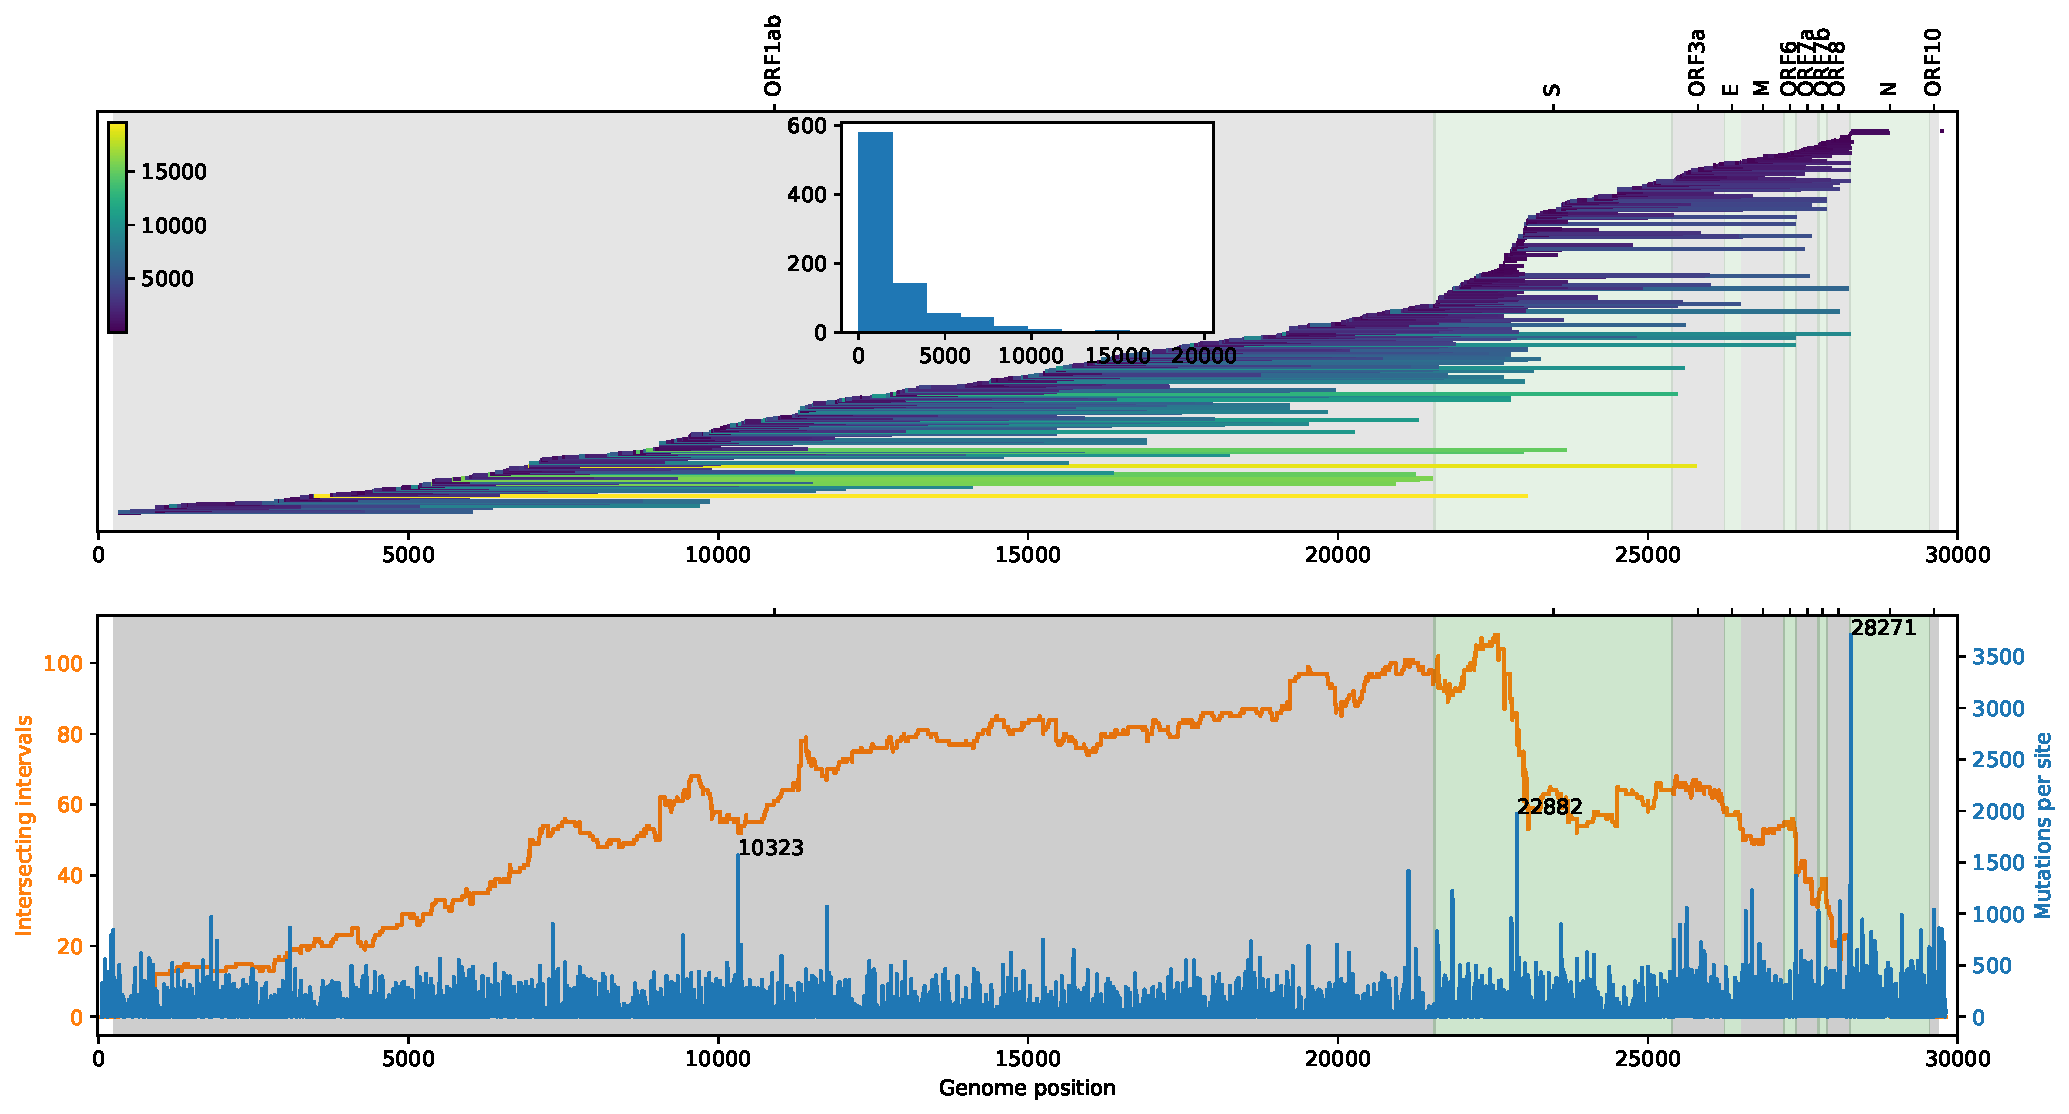
\includegraphics[width=\textwidth]{figures/long_arg_recombination_intervals.pdf}
\caption{\label{fig:long_arg_breakpoint_distribution}
Distribution of recombination breakpoints and mutations along the genome in
the Long ARG.
Top panel shows the intervals for 851 breakpoints associated
with 763 recombination nodes with at least two descending samples, plotted along the genome
as line segments (coloured by interval width).
Other details as described in Figure~\ref{fig:breakpoint-distribution}.}
\end{figure}


\begin{figure} \centering
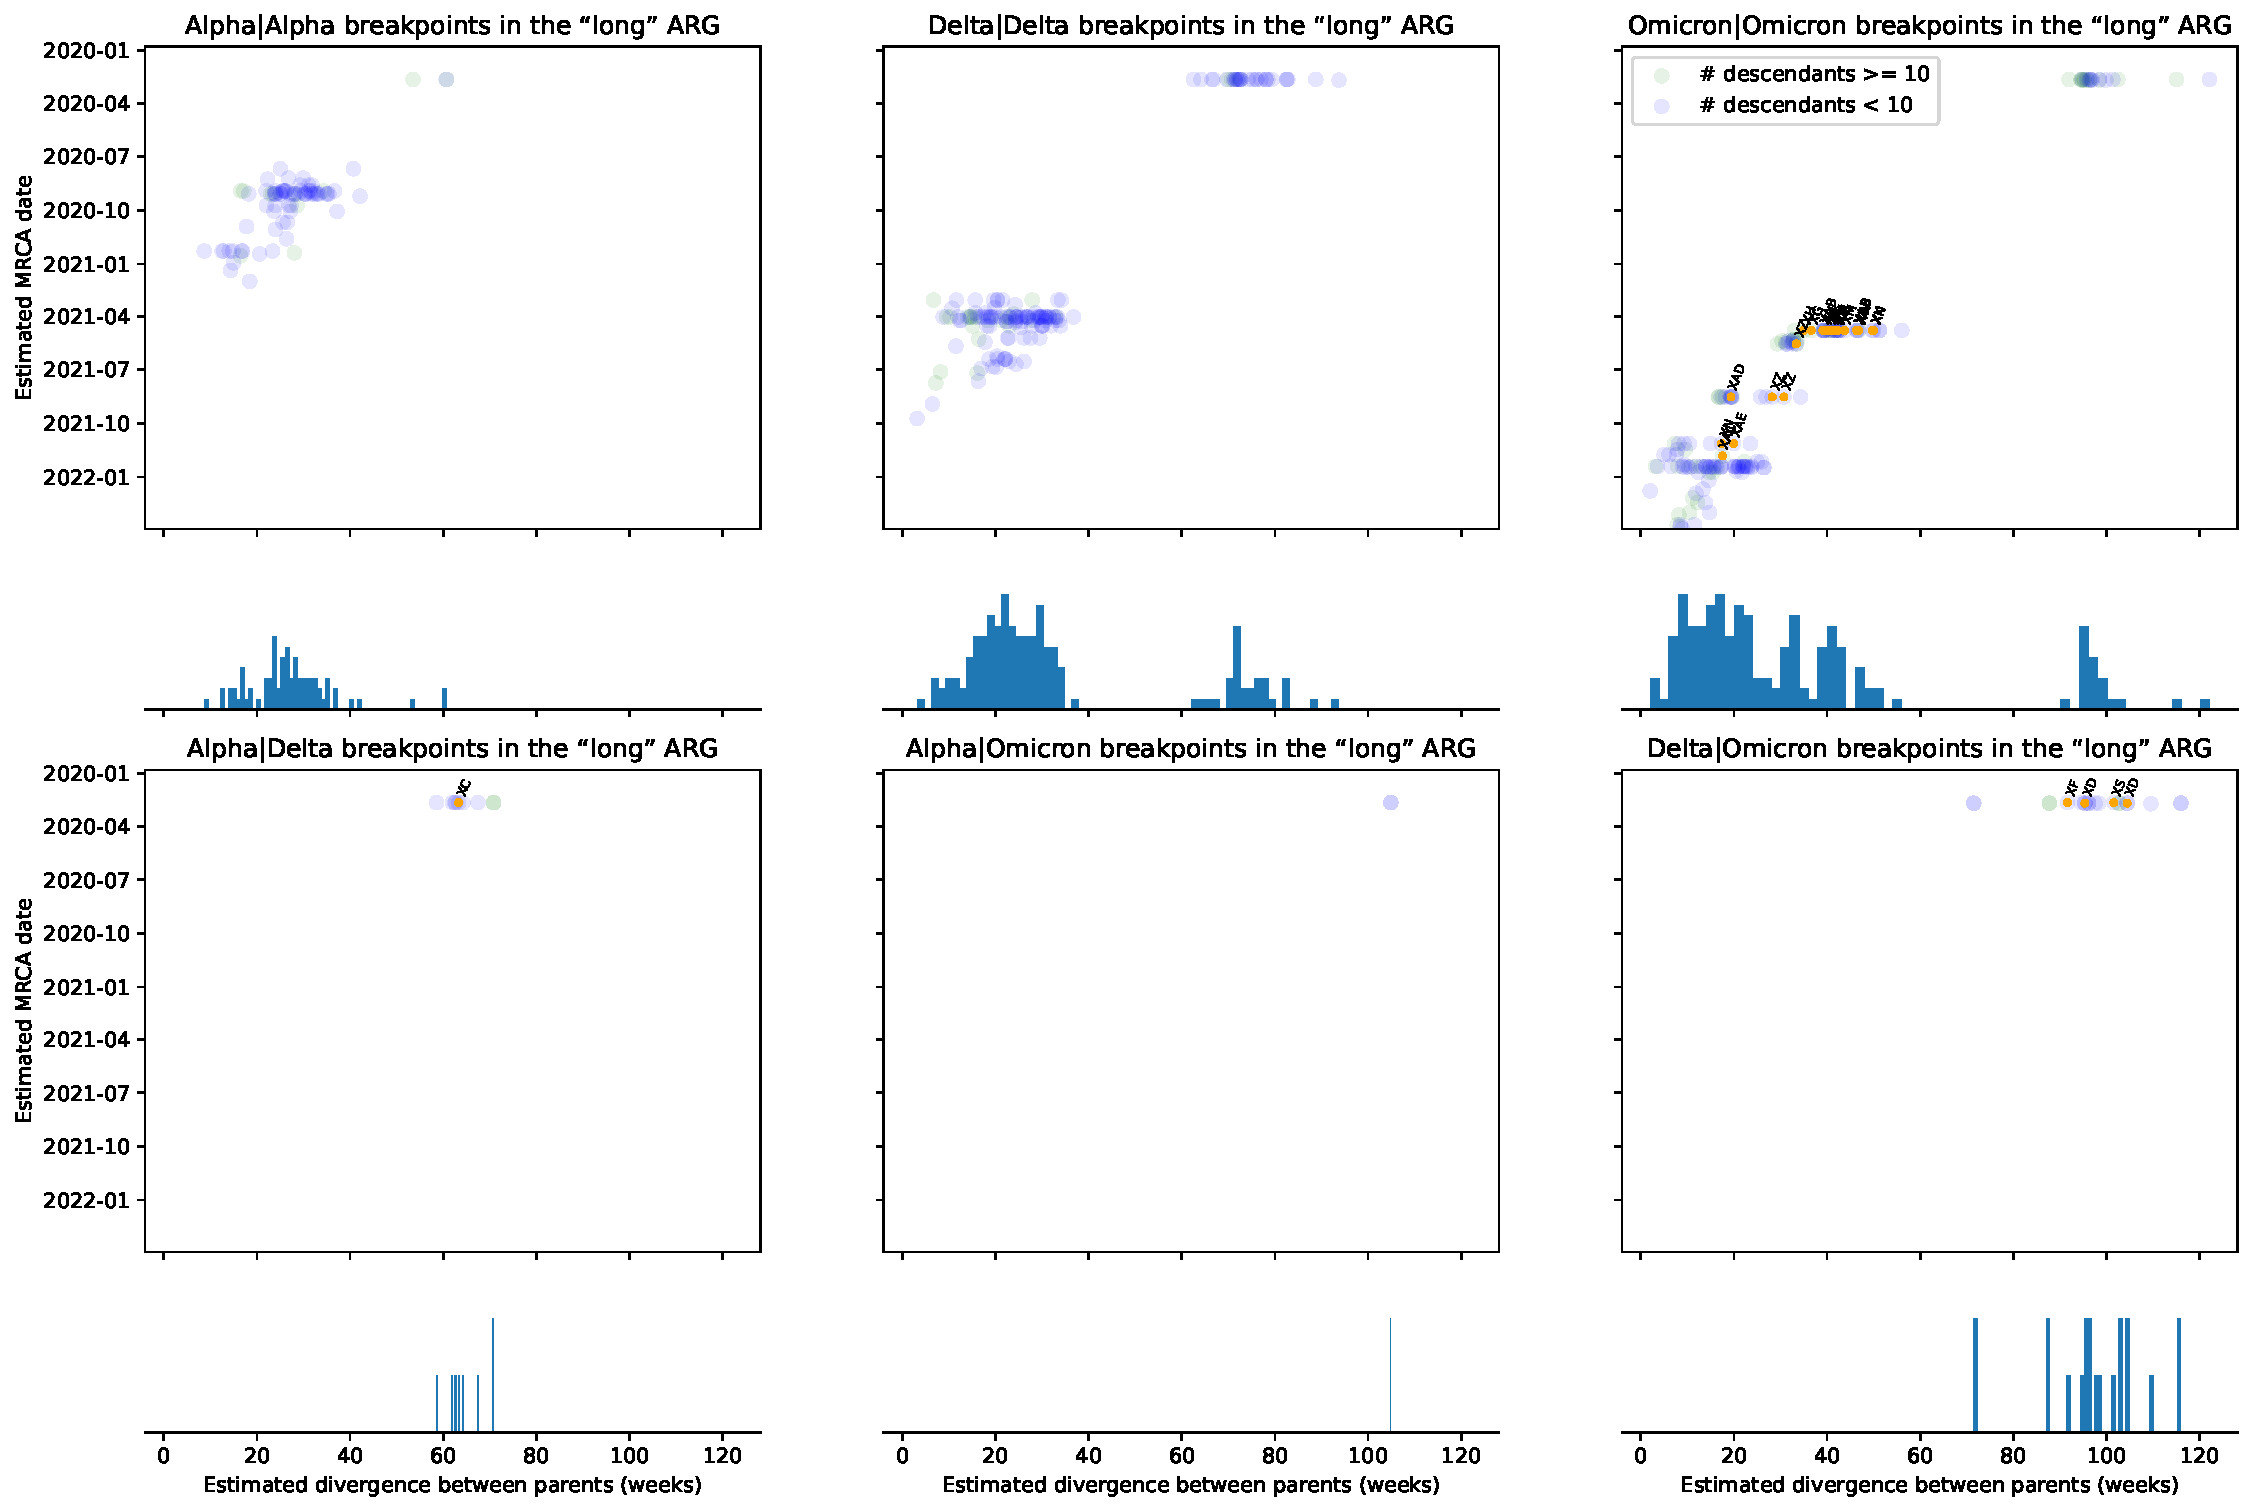
\includegraphics[width=\textwidth]{figures/supp_recombination_node_mrcas.pdf}
\caption{\label{fig:recomb_mrcas_voc_breakdown}  Divergence between parent
lineages for recombination events within and among different VoC categories.
There are 78 Alpha|Alpha recombination breakpoints corresponding to 75 recombination nodes 
(25 breakpoints / 24 nodes with $\geq5$ descendant samples).
148 breakpoints from 142 nodes are Delta|Delta recombinations (45 breakpoints / 45 nodes with  $\geq5$ descendants),
and 148 breakpoints from 142 nodes are Omicron|Omicron (71 breakpoints / 68 nodes with $\geq5$ descendants).
The equivalent figures for Alpha|Delta are 9 / 8 (3 / 2),
for Alpha|Omicron are 2 / 1 (0 / 0),
and for Delta|Omicron are 20 / 13 (6 / 3). 
Note that these plots do not include recombination breakpoints involving lineages that were not classified into these VoC categories.
}
\end{figure}

\begin{sidewaystable}
% \begin{footnotesize}
\centering
\begin{tabular}{p{1cm}p{1.2cm}p{4.2cm}lll}
\toprule
Focal Pango  & Num origins & Num focal samples (further split by origin, \textdagger=nested) & Official Pango parents & \textbf{Main clade}: sc2ts parents & \textbf{Main clade}: additional descendants \\
\midrule
\bfseries XA & 1 & \textbf{5} & B.1.1.7 + B.1.177 & B.1.1.7 + B.1.177.18 &  \\
\bfseries XF & 1 & \textbf{2} & B.1.617.2* + BA.1* & AY.4 + BA.1 &  \\
\bfseries XG & 1 & \textbf{32} & BA.1* + BA.2* & BA.1.17 + BA.2 & XAB: 1/48 \\
\bfseries XH & 1 & \textbf{11} & BA.1* + BA.2* & BA.1.20 + BA.2.9 & XAF: 34/35, B.1.1.529: 2, XE: 3/163 \\
\bfseries XK & 1 & \textbf{3} & BA.1* + BA.2* & BA.1.1.1 + BA.2 &  \\
\bfseries XL & 1 & \textbf{10} & BA.1* + BA.2* & BA.1.17.2 + BA.2 & XAB: 1/48, XU: 1/3 \\
\bfseries XR & 1 & \textbf{8} & BA.1.1* + BA.2* & BA.1.1 + BA.2 & XQ: 9/12, XAB: 2/48 \\
\bfseries XS & 1 & \textbf{4} & B.1.617.2* + BA.1.1* & AY.36 + BA.1.1 &  \\
\bfseries XT & 1 & \textbf{1} & BA.1* + BA.2* & BA.2.23 + Unknown & BA.2.23: 1 \\
\bfseries XV & 1 & \textbf{1} & BA.1* + BA.2* & BA.1.1 + BA.2 + Unknown & BA.2: 8 \\
\bfseries XW & 1 & \textbf{11} & BA.1* + BA.2* & BA.1.1.15 + BA.2 & XN: 2/13 \\
\bfseries XY & 1 & \textbf{6} & BA.1* + BA.2* & BA.1.1 + BA.2 & XAF: 1/35 \\
\bfseries XAA & 1 & \textbf{8} & BA.1* + BA.2* & BA.1 + BA.2.9 & XAB: 38/48, XAG: 17/17, XU: 1/3, XQ: 2/12 \\
\bfseries XAC & 1 & \textbf{27} & BA.1* + BA.2* & BA.1.17.2 + BA.2.3 &  \\
\bfseries XAE & 1 & \textbf{9} & BA.1* + BA.2* & BA.1 + BA.2 &  \\
\bfseries XAG & 1 & \textbf{17} & BA.1* + BA.2* & BA.1 + BA.2.9 & XAB: 38/48, XAA: 8/8, XU: 1/3, XQ: 2/12 \\
\bfseries XB & 2 & 57 (\textbf{57}, 1)\textdagger & B.1.631 + B.1.634 & B.1 + B.1.627 & B.1.634: 3, B.1.631: 7 \\
\bfseries XC & 2 & 3 (1, \textbf{2}) & AY.29 + B.1.1.7 & AY.103 + B.1.1.7 &  \\
\bfseries XD & 2 & 4 (1, \textbf{3}) & B.1.617.2* + BA.1* & AY.4 + BA.1.15 &  \\
\bfseries XJ & 2 & 2 (1, 1) & BA.1* + BA.2* & No main clade & No main clade \\
\bfseries XAD & 2 & 5 (1, \textbf{4}) & BA.1* + BA.2* & BA.1.1 + BA.2 &  \\
\bfseries XAF & 2 & 35 (\textbf{34}, 1) & BA.1* + BA.2* & BA.1.20 + BA.2.9 & XH: 11/11, B.1.1.529: 2, XE: 3/163 \\
\bfseries XAH & 2 & 12 (\textbf{10}, 2) & BA.1* + BA.2* & BA.1 + BA.2.10 & XZ: 61/66, XAD: 1/5 \\
\bfseries XQ & 3 & 12 (2, \textbf{9}, 1) & BA.1.1* + BA.2* & BA.1.1 + BA.2 & XR: 8/8, XAB: 2/48 \\
\bfseries XU & 3 & 3 (1, 1, 1) & BA.1* + BA.2* & No main clade & No main clade \\
\bfseries XM & 4 & 47 (2, 1, \textbf{40}, 4) & BA.1.1* + BA.2* & BA.1.1 + BA.2 &  \\
\bfseries XN & 4 & 13 (2, 2, \textbf{7}, 2) & BA.1* + BA.2* & BA.1 + BA.2 &  \\
\bfseries XAJ & 4 & 5 (1, 1, \textbf{3}, 1)\textdagger & BA.2.12.1* + BA.4* & Unknown & BA.5: 1 \\
\bfseries XE & 5 & 163 (3, \textbf{155}, 1, 3, 2)\textdagger & BA.1* + BA.2* & BA.1.17.2 + BA.2 &  \\
\bfseries XZ & 5 & 66 (1, 1, \textbf{61}, 2, 1) & BA.1* + BA.2* & BA.1 + BA.2.10 & XAH: 10/12, XAD: 1/5 \\
\bfseries XAB & 8 & 48 (1, \textbf{38}, 1, 2, 2, 2, 18, 2)\textdagger & BA.1* + BA.2* & BA.1 + BA.2.9 & XAA: 8/8, XAG: 17/17, XU: 1/3, XQ: 2/12 \\
\bottomrule
\end{tabular}
\caption{\label{tab:pango-recombinants}
Summary of the Pango X-lineages in the Long ARG (excluding XP and XAK whose samples are entirely filtered out, see text). In cases of multiple origins, most X-lineages have a single ``main clade'' (in bold).
Sc2ts inferred parents for the main clade are based on Nextclade designations, imputed where necessary.
Official parents are taken from Pango designation alias key (TODO: explain the asterisks). Note that B.1.617.2 is the origin of the Delta VoC, which includes all AY.* classes. Additional descendants within the main clade are summarised giving their NextClade Pango designation and clade count / total ARG count (the latter being omitted for non-recombinant designations).
}
\end{sidewaystable}

% \begin{table}
% \small
% \centering
% \begin{tabular}{lp{0.2cm}p{0.8cm}lp{0.9cm}ll}
% \toprule
% Date & $n$ & Causal Pango & Causal strain & Causal \#muts & Sc2ts parents & Breakpoint \\
% \midrule
% 2022-03-24 & 2 & XN & Germany/BY-RKI-I-674341/2022 & 3 & Unknown + BA.2 & (2833,9867) \\
% 2022-03-29 & 2 & XN & Spain/AB-HGUA-26086757/2022 & 2 & BA.1.1 + BA.2.9 & (2833,4185) \\
% 2022-04-23 & 7 & XN & Spain/MD-HRYC-12296321/2022 & 2 & BA.1 + BA.2 & (4185,4322) \\
% 2022-05-17 & 2 & XN & USA/TX-HMH-MCoV-97903/2022 & 5 & BA.2 + BA.2 & (22776,22787) \\
% \bottomrule
% \end{tabular}
% \caption{\label{tab:multiple_origins_table}
% Summary of inferred multiple ``origins'' for Nextclade-designated XN samples after filtering
% (Official: BA.1* \& BA.2*, breakpoint between 2834 \& 4183, defined from UK strains, earliest
% on 2022-02-01;  see \protect\url{https://github.com/cov-lineages/pango-designation/issues/480}).
% The 13 XN samples are grouped into rows based on their most recent ancestral recombination node;
% all the descendant samples of the four recombination nodes are designated XN by Nextclade.
% Details are also provided for the ``causal strain'' that led to the recombination
% being proposed by \texttt{sc2ts}. When undersampling causes three or more mutations to lie
% immediately above the causal strain, \texttt{sc2ts} may mistakenly propose multiple
% independent origins rather than one. Note that a large number of XN samples were previously
% removed by filtering.
% }
% \end{table}


\begin{figure} \centering
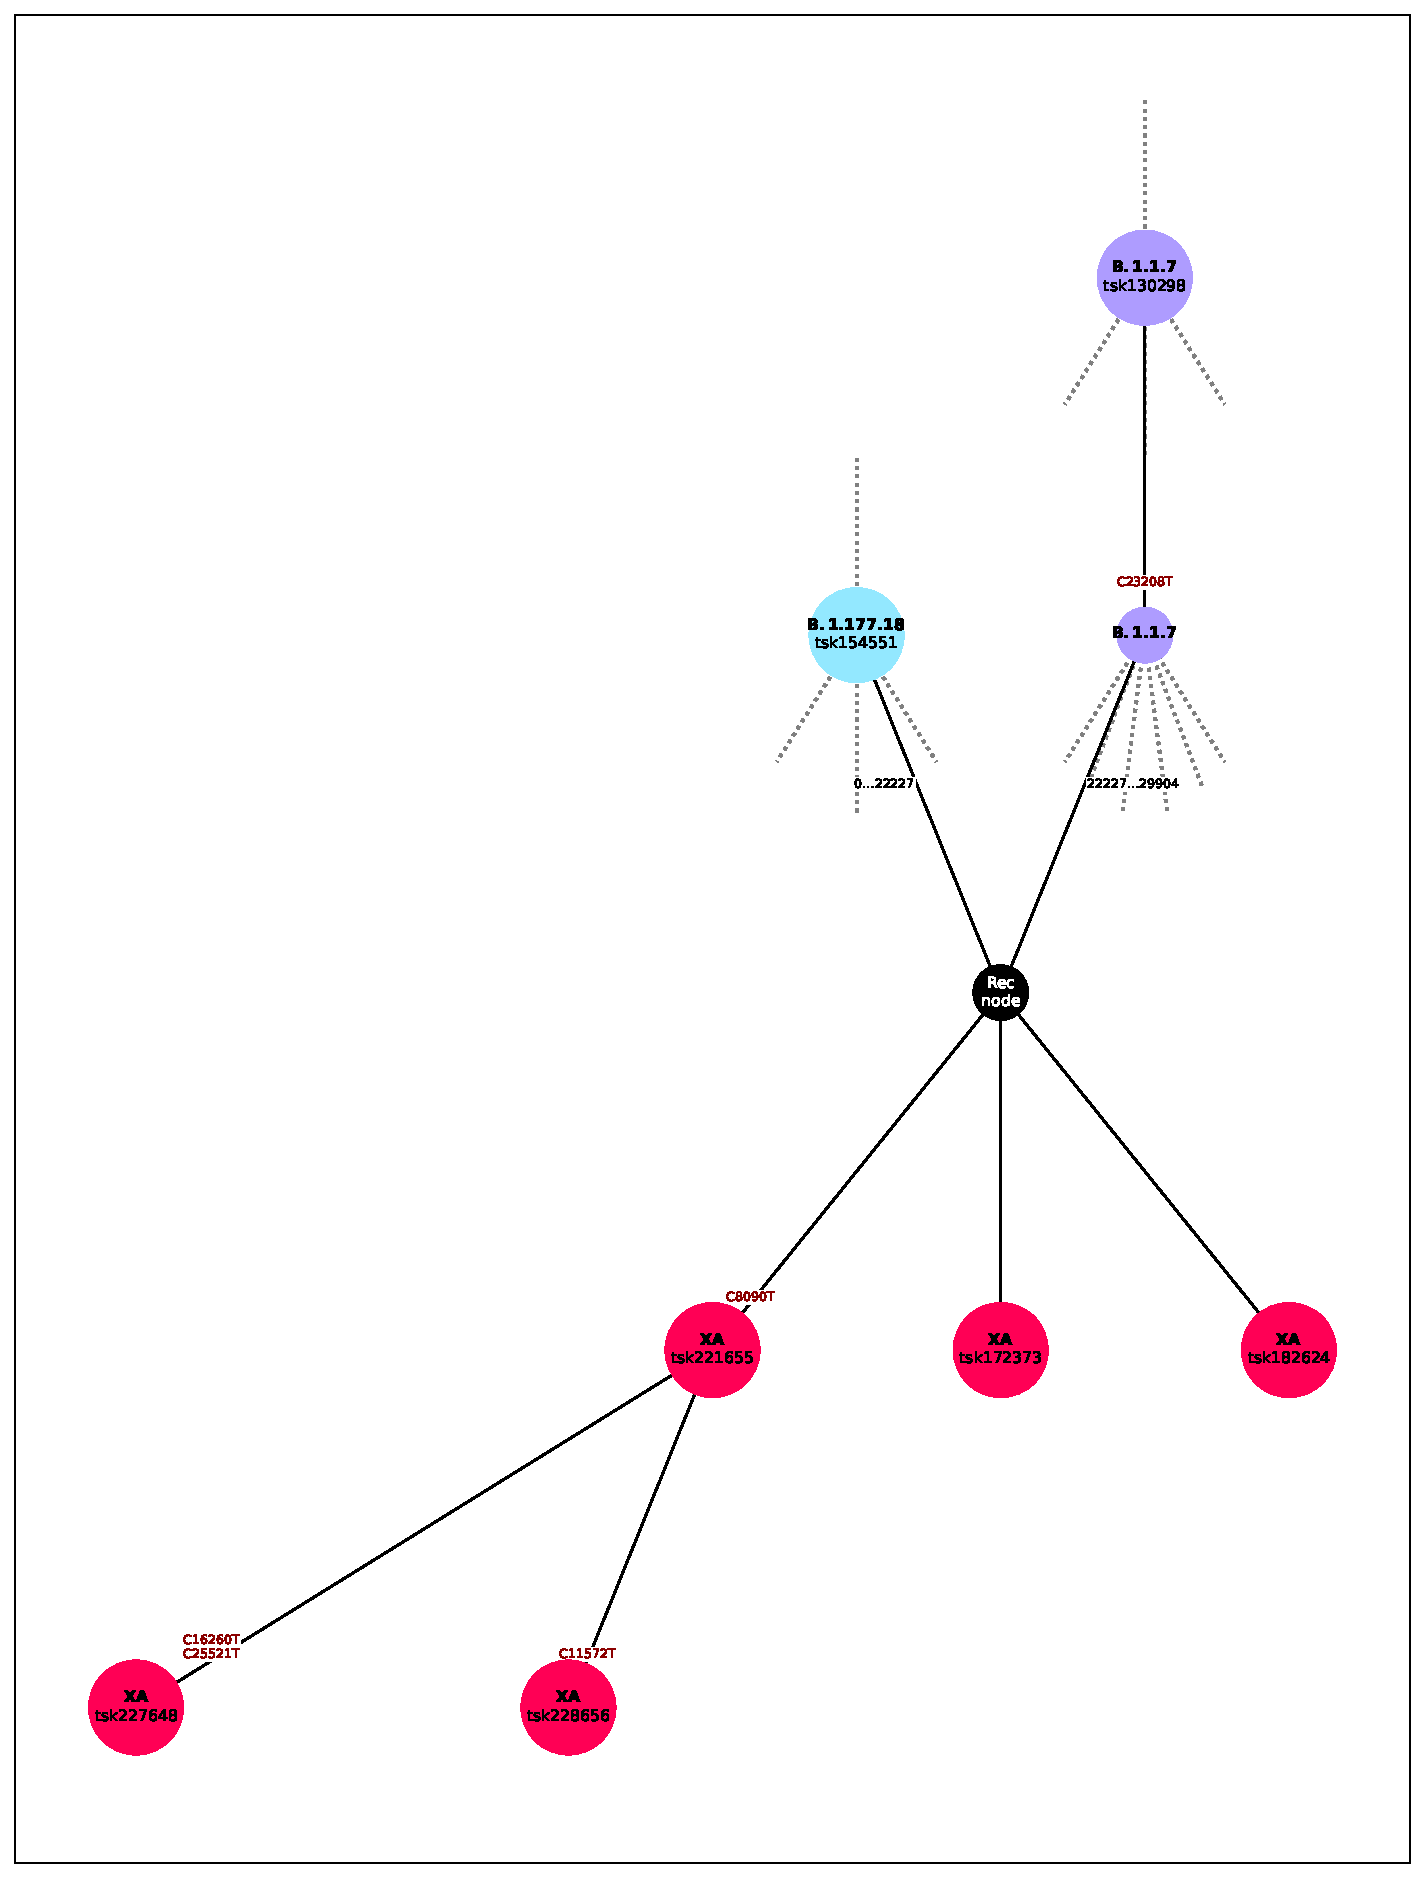
\includegraphics[width=0.5\textwidth]{figures/Pango_XA_gisaid_large_graph.pdf}
\caption{\label{fig:pango_XA_gisaid_graph}
Detailed version of Figure~\ref{fig:pango-simple-origin-graph}A. All single nucleotide mutations are listed
with the initial nucleotide state, followed by the reference genome position, followed by the derived
nucleotide state (after mutation). If an ancestral (``parent'') mutation exists at the same site in the path
to the root, it is possible for a mutation to be a ``reversion'' to the initial state of the parent mutation:
such reversions are indicated by lowercase nucleotide letters. Sample nodes are shown with \texttt{tskit} IDs,
which can be mapped to GISAID EPI ISL identifiers and strain names using supplementary file \protect\path{Pango_X_graph_sample_maps.txt}. In contrast to
Figure~\ref{fig:pango-simple-origin-graph}A, Pango lineages shown here are those assigned by GISAID rather
than Nextclade; however, in the specific case of XA, Nextclade and GISAID exactly agree on the lineage designations.
}
\end{figure}

\begin{sidewaysfigure} \centering
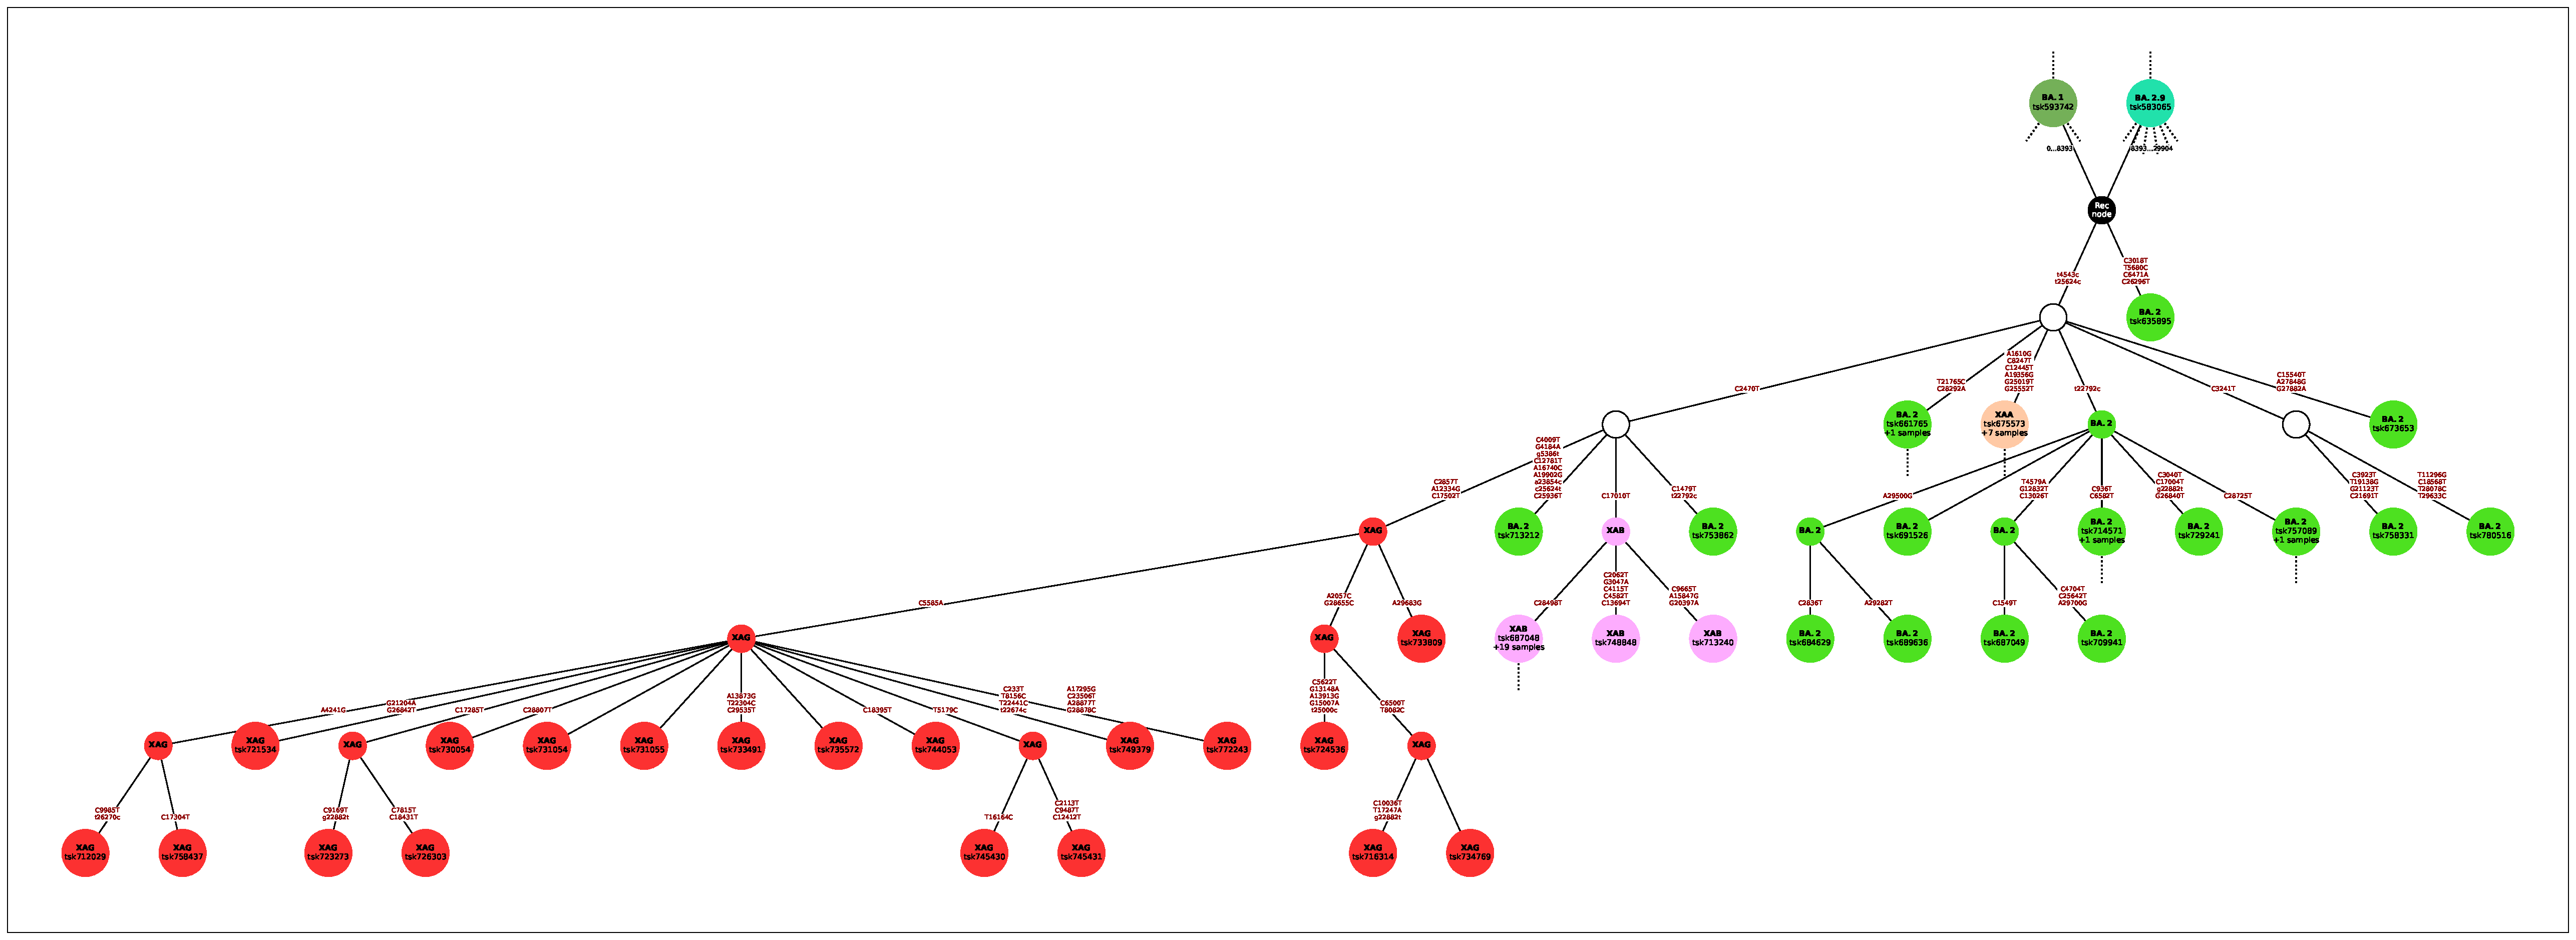
\includegraphics[width=\textwidth]{figures/Pango_XAG_gisaid_large_graph.pdf}
\caption{\label{fig:pango_XAG_gisaid_graph}
Detailed version of Figure~\ref{fig:pango-simple-origin-graph}B, with node and mutation labels as in
Figure~\ref{fig:pango_XA_gisaid_graph} (see supplementary file \protect\path{Pango_X_graph_sample_maps.txt}
to map tskID to EPI\_ISL and strain name).
Note that GISAID Pango designations assign an extra 2 samples to XAG, which are labelled as XAB
by Nextclade in Figure~\ref{fig:pango-simple-origin-graph}B. This renders XAG fully monophyletic.
However, unlike Nextclade, the GISAID designations also mark many of the samples in this subgraph
as non-recombinants (designating them BA.2), and in general we find that Nextclade assignments
agree more with our ARG structure than GISAID assignments.
}
\end{sidewaysfigure}

\begin{figure} \centering
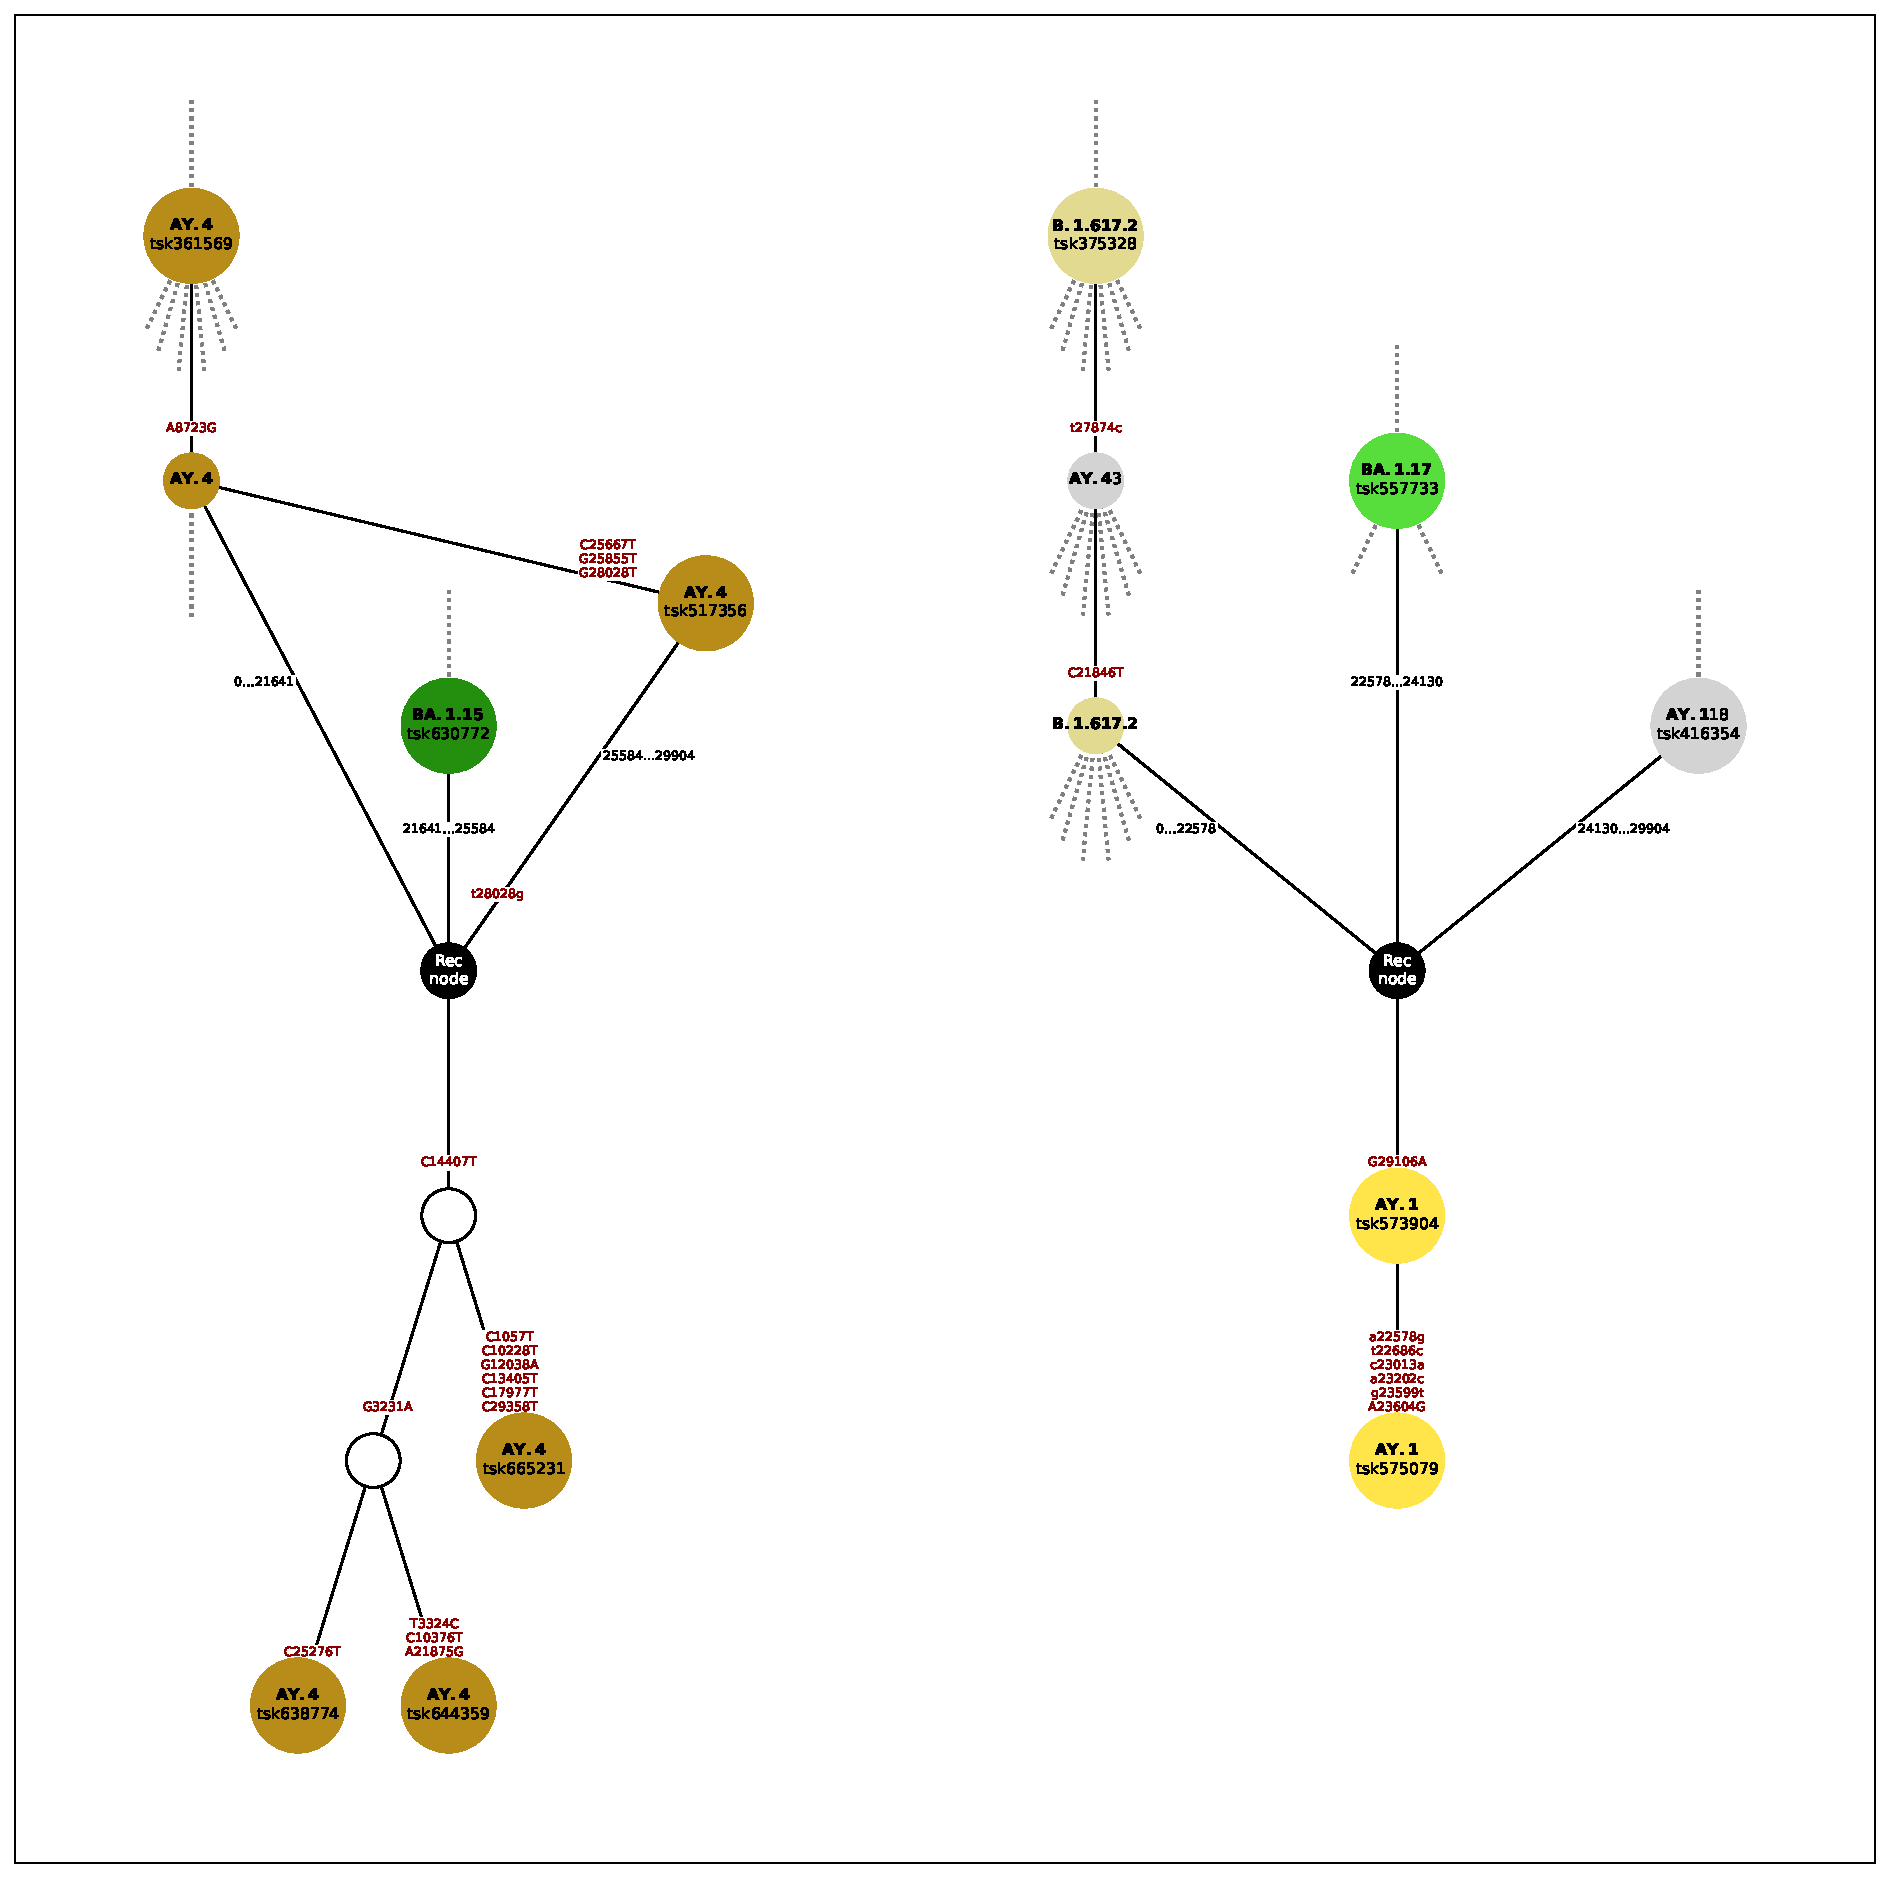
\includegraphics[width=0.6\textwidth]{figures/Pango_XD_gisaid_large_graph.pdf}
\caption{\label{fig:pango_XD_gisaid_graph}
Detailed version of Figure~\ref{fig:pango-simple-origin-graph}C, with node and mutation labels as in
Figure~\ref{fig:pango_XA_gisaid_graph} (see supplementary file \protect\path{Pango_X_graph_sample_maps.txt}
to map tskID to EPI\_ISL and strain name).
Note that GISAID does not designate any nodes as XD in the Long ARG, hence no recombinant Pango lineages
are marked in this plot. From inspection of the samples, we believe the GISAID designations to be erroneous
in this case.
}
\end{figure}

\begin{sidewaysfigure} \centering
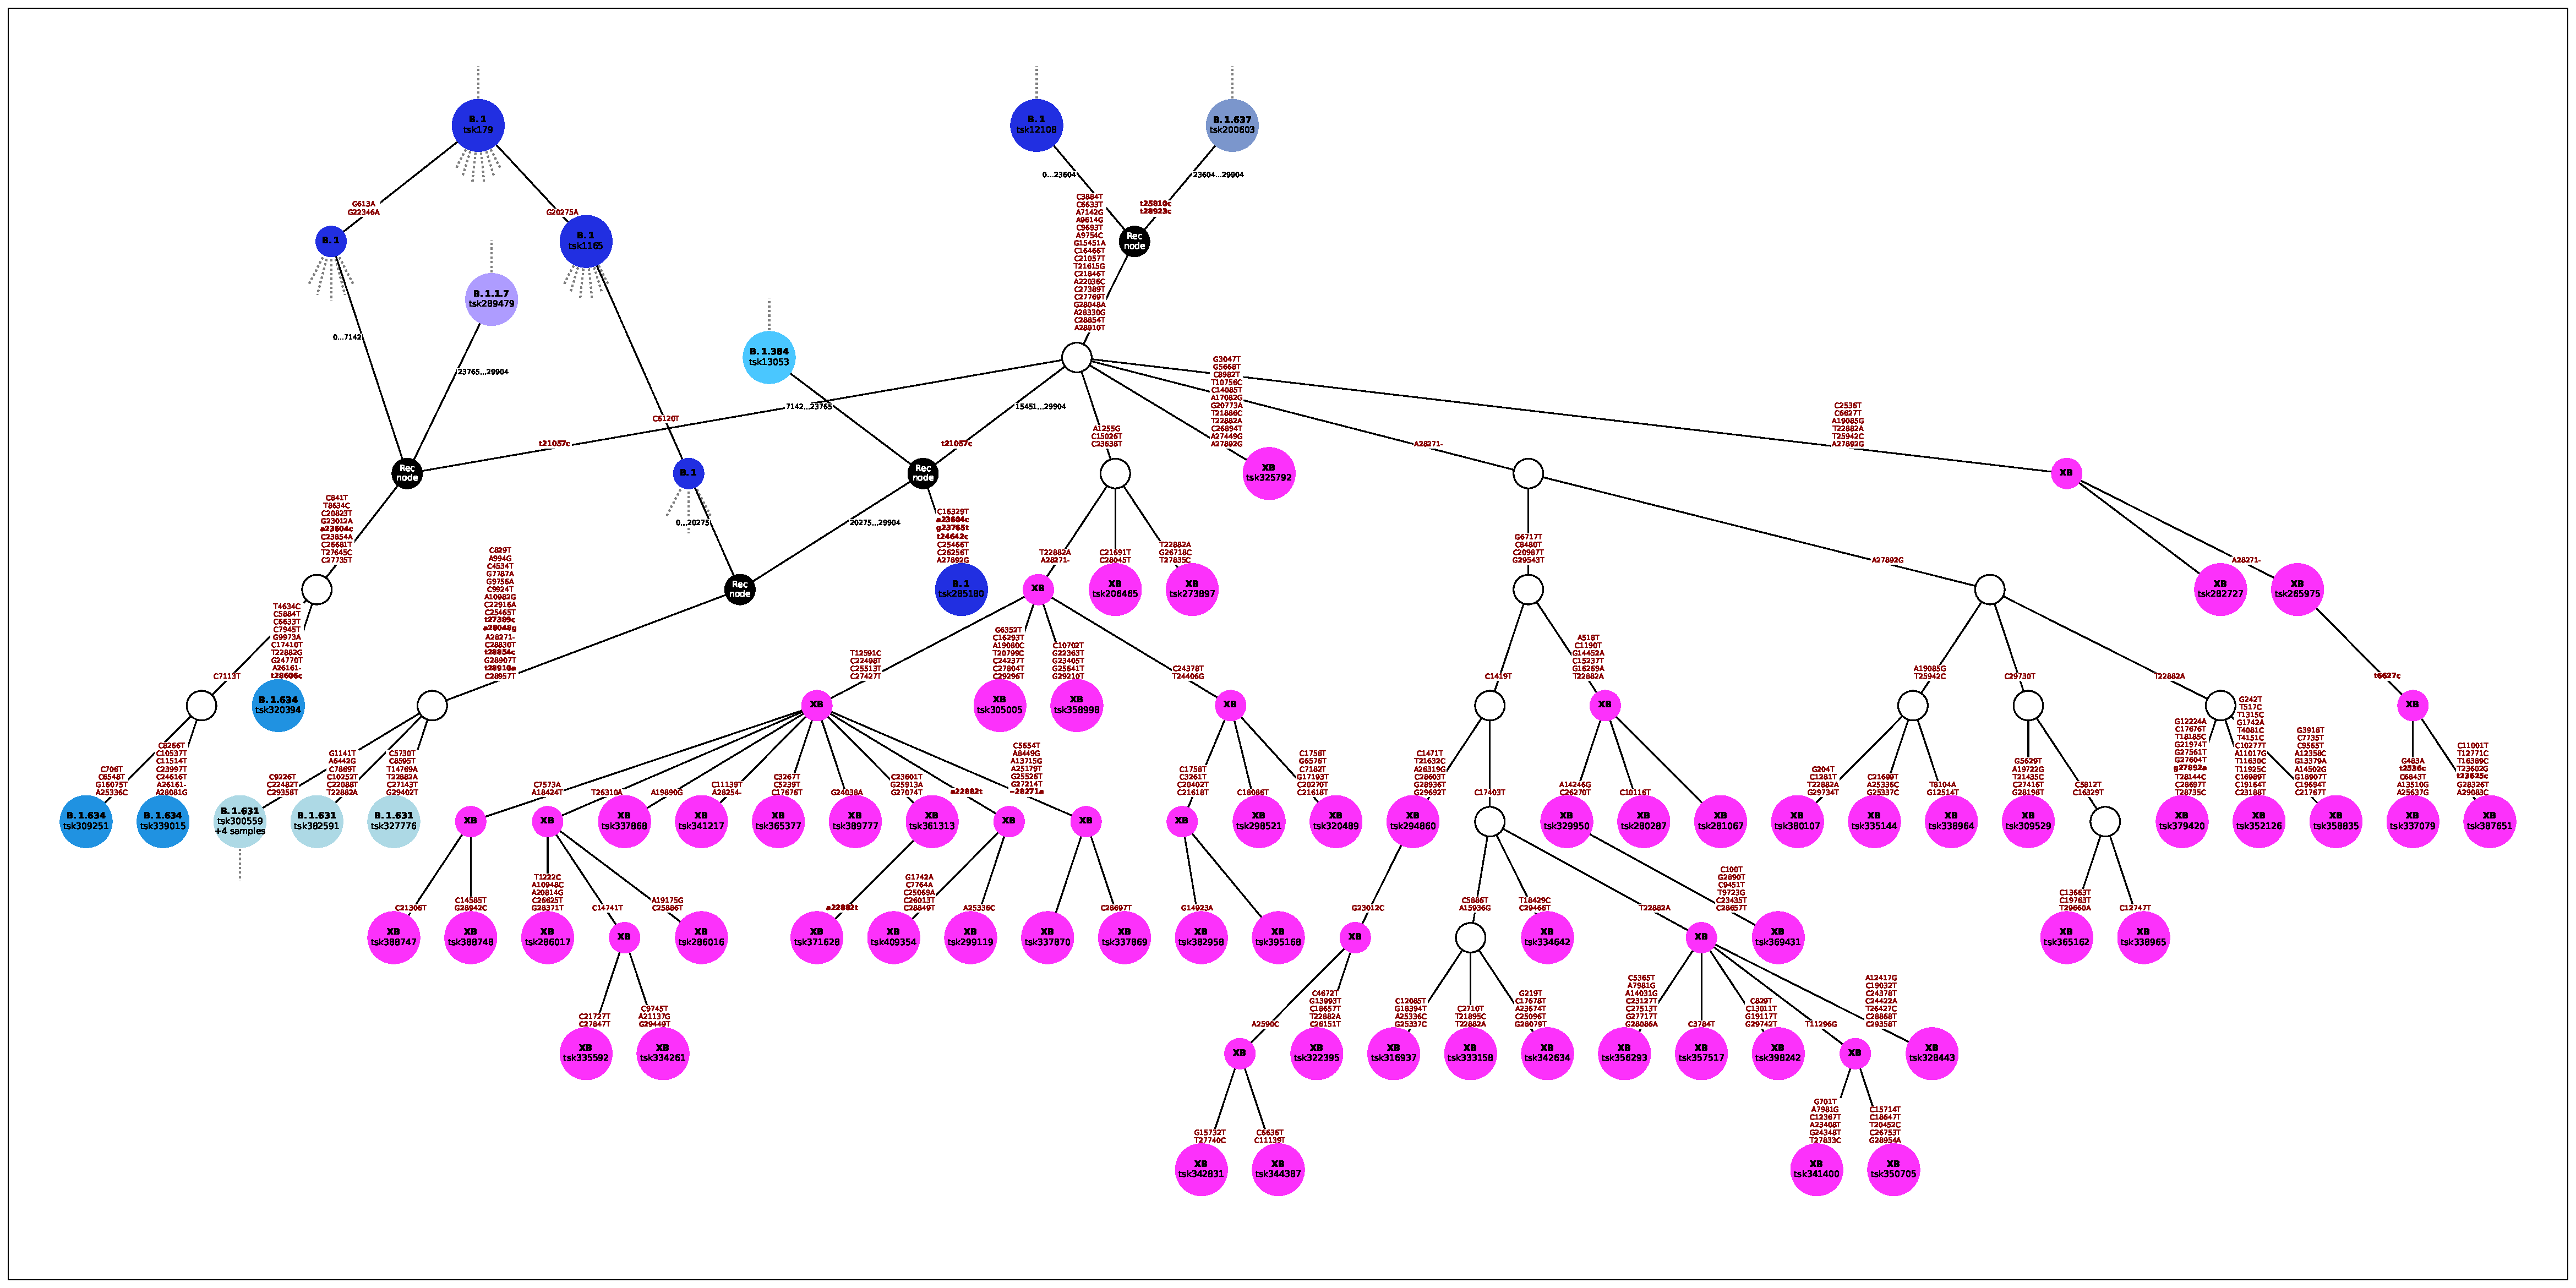
\includegraphics[width=\textwidth]{figures/Pango_XB_gisaid_large_graph.pdf}
\caption{\label{fig:pango_XB_gisaid_graph}
Detailed version of Figure~\ref{fig:complex_origins_graph}, with node and mutation labels as in
Figure~\ref{fig:pango_XA_gisaid_graph} (see supplementary file \protect\path{Pango_X_graph_sample_maps.txt}
to map tskID to EPI\_ISL and strain name).
The GISAID XB designations agree with the Nextclade ones except in two cases: an unplotted
singleton recombinant nested within the main grouping, and the tsk285180 node marked BA.1 in this plot,
but which is labelled XB by Nextstrain.
}
\end{sidewaysfigure}

%% Could insert the Pango_X_graph_sample_maps.txt with something like this
%% but maybe best to leave it as a separate file?
%% \lstinputlisting[caption={XXX}]{data/Pango_X_graph_sample_maps.txt}

\end{document}
